\documentclass[11pt,a4paper,openright]{report}

\usepackage[utf8]{inputenc}
\usepackage[italian]{babel}
\usepackage[T1]{fontenc}
\usepackage{geometry}
\geometry{a4paper, top=3cm, bottom=3cm, left=3cm, right=3cm}
\usepackage{graphicx}
\usepackage{hyperref}
\usepackage{amsmath,amssymb}
\usepackage{booktabs}
\usepackage{listings}
\usepackage{xcolor}
\usepackage{float}
\usepackage{microtype}
\usepackage{pdflscape}
\usepackage{tikz}
\usetikzlibrary{shapes.geometric,shapes.multipart,arrows.meta,positioning,fit,calc}
% small set of tikz styles to draw uml class diagrams by hand.
% every box is a node, every relation is a \draw with one of the styles below.

\usetikzlibrary{shapes.multipart, arrows.meta, positioning, calc}

\definecolor{umlhead}{RGB}{226, 234, 245}
\definecolor{umlline}{RGB}{40, 40, 40}

\tikzset{
  % box with two parts: name (with stereotype) and operations
  uml/.style={
    rectangle split, rectangle split parts=2,
    rectangle split part align={center, left},
    rectangle split part fill={umlhead, white},
    draw=umlline, minimum width=#1, align=left, inner sep=3pt,
    font=\sffamily\footnotesize, anchor=north
  },
  uml/.default=4.6cm,
  % box with only the name, for classes already shown in another figure
  umlref/.style={
    rectangle, draw=umlline, fill=umlhead, dashed,
    font=\sffamily\footnotesize, minimum width=3cm, minimum height=0.8cm,
    align=center, anchor=north
  },
  every uml relation/.style={draw=umlline, semithick},
  extends/.style={every uml relation, -{Triangle[open, length=3mm, width=3mm]}},
  implements/.style={every uml relation, dashed, -{Triangle[open, length=3mm, width=3mm]}},
  association/.style={every uml relation, -{Stealth[length=2.5mm]}},
  composition/.style={every uml relation, {Diamond[length=3.5mm, width=2.4mm]}-{Stealth[length=2.5mm]}},
  aggregation/.style={every uml relation, {Diamond[open, length=3.5mm, width=2.4mm]}-{Stealth[length=2.5mm]}},
  dependency/.style={every uml relation, dashed, -{Stealth[length=2.5mm]}},
  rel/.style={font=\sffamily\scriptsize, inner sep=1.5pt},
}

% header colors, one for each area of the application (used by the global domain diagram)
\definecolor{areaCurrency}{RGB}{220, 232, 247}
\definecolor{areaWallet}{RGB}{215, 240, 236}
\definecolor{areaDashboard}{RGB}{226, 243, 218}
\definecolor{areaInvest}{RGB}{253, 233, 210}
\definecolor{areaMarket}{RGB}{236, 226, 248}
\definecolor{areaSettings}{RGB}{232, 232, 232}

% \umlarea{color}: the next boxes get this header color
\newcommand{\umlarea}[1]{\colorlet{umlhead}{#1}}

% no hyphenation inside the boxes: method names must stay whole
\newcommand{\umlnohyphen}{\hyphenpenalty=10000\exhyphenpenalty=10000\relax}

% \umlclass[width]{node id}{position}{stereotype}{name}{operations, one per line separated by \\}
% the stereotype can be empty (plain class). abstract methods: write them inside \umlabstract{...}
\newcommand{\umlclass}[6][4.6cm]{%
  \node[uml=#1] (#2) at (#3) {%
    \ifx\relax#4\relax\else{\scriptsize\guillemotleft #4\guillemotright}\\\fi\textbf{#5}%
    \nodepart{second}\umlnohyphen#6};%
}

% shortcut for interfaces
\newcommand{\umlinterface}[5][4.6cm]{\umlclass[#1]{#2}{#3}{interface}{#4}{#5}}

% abstract operation (italic, as in uml)
\newcommand{\umlabstract}[1]{\textit{#1}}

% \umlref{node id}{position}{name}: class already shown in another figure, name only
\newcommand{\umlref}[3]{%
  \node[umlref] (#1) at (#2) {\textbf{#3}};%
}


\hypersetup{
    colorlinks=true,
    linkcolor=blue!70!black,
    citecolor=blue!70!black,
    urlcolor=blue!70!black
}

\lstset{
    basicstyle=\small\ttfamily,
    breaklines=true,
    frame=single,
    numbers=left,
    numberstyle=\tiny\color{gray},
    keywordstyle=\color{blue}\bfseries,
    commentstyle=\color{gray}\itshape,
    stringstyle=\color{teal},
    backgroundcolor=\color{gray!5}
}

\title{\textbf{UniBodget — Relazione di Progetto} \\
\large Corso di Programmazione ad Oggetti --- A.A. 2025/2026}
\author{%
  \textbf{Arianna Palmucci}\\{\small\texttt{arianna.palmucci@studio.unibo.it}}
  \and
  Daniele Zappalà\\{\small\texttt{daniele.zappala3@studio.unibo.it}}
  \and
  Favour Emuwahen\\{\small\texttt{favour.emuwahen@studio.unibo.it}}
}
\date{Ottobre 2026}

\begin{document}

\maketitle

\chapter*{Sommario}
La presente relazione documenta l'analisi, la progettazione architetturale, lo sviluppo implementativo e la verifica del progetto software \textbf{UniBodget}, un'applicazione desktop modulare in Java finalizzata alla gestione completa delle finanze personali, della contabilità multi-asset, del monitoraggio di portafogli d'investimento e della conversione multivaluta in tempo reale.

Il documento è redatto in rigorosa aderenza alla struttura prescritta dalla \emph{Meta-relazione per Programmazione ad Oggetti} (Prof. Danilo Pianini). In particolare, vengono analizzati e dettagliati i seguenti sottosistemi architetturali:
\begin{enumerate}
    \item Il sottosistema del dominio valute (\emph{fiat}, \emph{crypto}, \emph{stock}, \emph{custom}) e il relativo motore polimorfico di conversione;
    \item L'infrastruttura di integrazione con API di mercato esterne, supportata da una cache trasparente resiliente e meccanismi di fallback;
    \item Il monitoraggio continuo dei tassi, con watchlist interattiva e sistema reattivo di allerte visive su soglie critiche;
    \item Il modulo grafico dedicato al convertitore di valute (\texttt{CurrencyConverterModule}), comprendente il simulatore di cambio bancario con spread e commissioni fisse;
    \item La gestione trasversale delle preferenze dell'utente (\texttt{SettingsController}), dei temi dinamici con iniezione CSS in tempo reale (\texttt{ThemeManager}) e della persistenza affidabile dello stato applicativo su file JSON strutturati.
\end{enumerate}

\tableofcontents

% ============================================================================
% CAPITOLO 1: ANALISI
% ============================================================================
\chapter{Analisi}

\section{Descrizione e requisiti}

UniBodget è un'applicazione desktop per la gestione delle finanze personali. Il suo scopo è riunire in
un unico posto il denaro usato tutti i giorni (contanti, conti correnti, carte) e il patrimonio investito
(azioni e criptovalute), anche quando questi sono espressi in valute diverse.

Oggi una persona tiene spesso i propri soldi su più canali: uno o più conti in euro, magari un conto in
un'altra valuta, un broker per le azioni e un exchange per le criptovalute. Ognuno di questi ha la propria
interfaccia e la propria unità di misura, per cui rispondere a domande semplici come ``quanto ho speso
questo mese?'' o ``i miei investimenti stanno guadagnando o perdendo?'' richiede di consultare più
strumenti e di fare conversioni a mano. UniBodget vuole rispondere a queste domande da un'unica
applicazione, che lavora sul computer dell'utente senza richiedere l'accesso ai suoi conti bancari.

\subsection*{Glossario}

\begin{description}
  \item[Valuta (o unità di valore)] qualunque cosa in cui si può esprimere una quantità di denaro o di
    patrimonio. Si distinguono tre tipi: valute \emph{fiat} (euro, dollaro, ...), \emph{criptovalute}
    (bitcoin, ether, ...) e \emph{azioni} quotate in borsa, identificate dal loro simbolo (es.\ AAPL).
  \item[Stablecoin] criptovaluta il cui valore è agganciato a una valuta fiat (es.\ USDT, circa
    1~dollaro). Può essere usata come ``liquidità'' all'interno di un conto di investimento.
  \item[Importo] una quantità associata a una valuta, ad esempio 12,50~EUR oppure 0,003~BTC.
  \item[Conto] contenitore di denaro o di patrimonio con un nome e una \emph{valuta di riferimento}, in
    cui vengono espressi i suoi totali. I conti sono di due tipi:
    \begin{itemize}
      \item \emph{conto di liquidità}: denaro per le spese di tutti i giorni (es.\ conto corrente,
        contanti); il suo saldo è la somma dei movimenti registrati;
      \item \emph{conto di investimento}: contiene azioni e criptovalute; il suo valore dipende dai
        prezzi di mercato del momento.
    \end{itemize}
  \item[Movimento (o transazione)] registrazione di un'operazione su un conto: un'entrata, una spesa, un
    trasferimento, un prestito a un amico, oppure un acquisto o una vendita di un titolo.
  \item[Categoria] etichetta che classifica un movimento (es.\ ``Spesa alimentare'', ``Stipendio''), con
    un colore e un tipo (entrata, uscita, trasferimento, prestito).
  \item[Posizione] quanto si possiede di un certo titolo in un conto di investimento, con il suo
    \emph{prezzo medio di carico}, cioè il prezzo medio pagato per acquistarlo.
  \item[Costo di carico] quanto è stato speso in totale per acquistare le posizioni ancora aperte.
  \item[Profitto/perdita (P/L)] differenza tra valore e costo. È \emph{non realizzato} finché il titolo
    è ancora posseduto, \emph{realizzato} quando viene venduto.
  \item[Spread] maggiorazione percentuale che una banca applica al tasso di cambio di mercato quando
    converte denaro da una valuta a un'altra, spesso insieme a una commissione fissa.
  \item[Budget] limite di spesa mensile fissato dall'utente per un conto di liquidità, con una soglia di
    avviso espressa in percentuale del limite.
  \item[Cruscotto (dashboard)] schermata di riepilogo di un conto di liquidità: saldo, budget, spese per
    categoria, prestiti, confronti con il mese precedente e movimenti recenti.
  \item[Prestito ad amici] denaro dato a un amico (o restituito da lui) che l'utente vuole tracciare, per
    sapere in ogni momento quanto deve ancora ricevere.
  \item[Confronto mensile (insight)] indicatore che confronta un valore del mese corrente (spese, entrate,
    risparmi) con quello del mese precedente, indicando se l'andamento è positivo, negativo o stabile.
  \item[Watchlist] elenco di coppie di valute che l'utente vuole tenere sotto controllo.
\end{description}

\subsection*{Requisiti funzionali}

\paragraph{Conti e movimenti}
\begin{itemize}
  \item L'utente può creare, rinominare ed eliminare più conti di liquidità, ognuno con la propria valuta
    di riferimento.
  \item L'utente può registrare entrate, spese, trasferimenti e prestiti fatti a (o ricevuti da) amici,
    indicando importo, data, categoria e una descrizione.
  \item Un movimento registrato per errore può essere corretto o eliminato.
  \item Oltre alle categorie predefinite, l'utente può creare categorie personalizzate con nome, tipo e
    colore.
  \item Lo storico dei movimenti si può cercare per parola chiave e filtrare per categoria, tipo e
    intervallo di date, ordinandolo in modi diversi.
  \item Lo storico di un conto si può esportare in un file leggibile da un foglio di calcolo.
\end{itemize}

\paragraph{Cruscotto, budget e prestiti}
\begin{itemize}
  \item L'utente sceglie il conto di liquidità da consultare; il cruscotto ne mostra il saldo, lo stato
    del budget, la ripartizione delle spese, i prestiti aperti, i confronti mensili e gli ultimi
    movimenti, e si aggiorna subito a ogni modifica.
  \item Per ogni conto di liquidità l'utente può fissare un budget mensile e una soglia di avviso
    (es.\ l'80\% del limite). L'applicazione indica quanta parte del budget è stata usata e in quale stato
    si trova la spesa del mese: \emph{nella norma}, \emph{in avviso} (soglia superata) o \emph{critica}
    (limite raggiunto o superato).
  \item L'applicazione mostra come si ripartiscono le spese del mese tra le categorie, sia in percentuale
    sia come elenco delle categorie in cui si spende di più.
  \item L'applicazione confronta spese, entrate e risparmi del mese corrente con quelli del mese
    precedente, mostrando la differenza in valore e in percentuale e se l'andamento è positivo o negativo.
  \item L'utente può registrare un prestito fatto a un amico e, in seguito, le sue restituzioni (anche
    parziali). Per ogni amico l'applicazione riassume quanto è stato prestato, quanto è stato restituito e
    quanto resta da ricevere.
\end{itemize}

\paragraph{Investimenti}
\begin{itemize}
  \item L'utente può creare, rinominare ed eliminare più conti di investimento.
  \item L'utente può registrare acquisti e vendite di azioni e criptovalute, indicando quantità, prezzo
    unitario e commissioni, e può trasferire un titolo da un conto di investimento a un altro.
  \item Un acquisto può essere pagato con un conto di liquidità, con una stablecoin posseduta nello stesso
    conto, oppure con fondi esterni non gestiti dall'applicazione. Allo stesso modo, il ricavato di una
    vendita può essere accreditato su un conto di liquidità o in stablecoin.
  \item Un ordine che non può essere eseguito (fondi insufficienti, quantità da vendere maggiore di quella
    posseduta, ...) deve essere rifiutato, spiegando il motivo all'utente, senza modificare nessun conto.
  \item Per ogni posizione l'applicazione mostra quantità, prezzo medio di carico, valore di mercato
    attuale e profitto/perdita non realizzato.
  \item Per ogni conto di investimento l'applicazione mostra il valore totale, il costo di carico, il
    profitto/perdita complessivo (realizzato e non realizzato) in valore e in percentuale, e i titoli con il
    rendimento migliore e peggiore.
  \item L'applicazione mostra come il conto è ripartito tra i titoli, sia per valore sia per quantità.
  \item L'applicazione mostra l'andamento nel tempo del profitto/perdita del conto: il valore viene
    registrato dopo ogni operazione e periodicamente mentre l'applicazione è aperta.
  \item Lo storico delle operazioni di un conto di investimento si può esportare in un file leggibile da
    un foglio di calcolo.
\end{itemize}

\paragraph{Conversione di valute e mercati}
\begin{itemize}
  \item L'utente può convertire un importo tra due valute qualsiasi tra quelle supportate (fiat,
    criptovalute e azioni), al tasso di mercato corrente.
  \item L'utente può simulare il cambio di denaro presso diverse banche, vedendo spread, commissione fissa
    e importo che riceverebbe davvero.
  \item L'utente può vedere in un grafico l'andamento del tasso di cambio di una coppia di valute in un
    intervallo di date scelto.
  \item L'utente può salvare coppie di valute preferite in una watchlist, per vederne subito il tasso.
  \item L'utente può impostare un avviso su una coppia di valute: quando il tasso supera la soglia
    impostata, l'applicazione lo segnala.
\end{itemize}

\paragraph{Preferenze}
\begin{itemize}
  \item L'utente sceglie una valuta di riferimento globale, in cui vengono mostrati i totali che
    riuniscono più conti.
  \item L'utente può passare tra tema chiaro e tema scuro e cambiare il carattere del testo; le modifiche
    si vedono subito, senza riavviare l'applicazione.
  \item L'applicazione ricorda dimensione e posizione della finestra tra un avvio e l'altro.
  \item L'utente può salvare la configurazione corrente e tornare in seguito a una configurazione
    salvata in precedenza.
\end{itemize}

\paragraph{Dati}
\begin{itemize}
  \item Ogni modifica (conti, movimenti, categorie, preferenze) viene salvata automaticamente, senza
    un comando esplicito dell'utente, e ritrovata al successivo avvio.
  \item Al primo avvio, senza dati salvati, l'applicazione parte da uno stato vuoto ma funzionante.
\end{itemize}

\subsection*{Requisiti non funzionali}

\begin{itemize}
  \item \textbf{Precisione}: i calcoli sugli importi devono essere esatti, senza gli errori di
    arrotondamento tipici dei numeri in virgola mobile. Ogni valuta va mostrata con il numero di decimali
    adatto (2 per l'euro, fino a 8 per le criptovalute).
  \item \textbf{Coerenza dei dati}: saldi e statistiche devono essere sempre coerenti con lo storico dei
    movimenti, anche dopo una correzione o una cancellazione. Un'operazione che coinvolge due conti (ad
    esempio un acquisto pagato con un conto di liquidità) deve modificarli entrambi oppure nessuno.
  \item \textbf{Robustezza verso i servizi esterni}: i prezzi di mercato arrivano da servizi pubblici e
    gratuiti, che possono essere lenti, limitare il numero di richieste o non essere raggiungibili.
    L'applicazione deve continuare a funzionare anche in questi casi (ad esempio mostrando l'ultimo prezzo
    noto) e non deve mai perdere dati dell'utente. Non è richiesto che i prezzi siano in tempo reale: un
    ritardo dell'ordine di un'ora è accettabile.
  \item \textbf{Privacy}: tutti i dati restano sul computer dell'utente; non servono registrazioni né
    credenziali bancarie.
  \item \textbf{Portabilità}: l'applicazione deve funzionare su Windows, macOS e Linux senza modifiche.
  \item \textbf{Estendibilità}: deve essere possibile aggiungere nuovi tipi di valuta o di mercato, nuove
    categorie e nuove fonti di prezzi senza riscrivere le parti esistenti.
\end{itemize}

\section{Modello del dominio}
\enlargethispage{2\baselineskip}

Il modello del dominio è riassunto in Figura~\ref{fig:dominio-conti} e Figura~\ref{fig:dominio-mercato}, dove le entità sono suddivise tra la gestione dei conti, storico e budget (Parte~1) e l'ecosistema di mercato, tassi e valute (Parte~2). Di seguito le aree sono descritte una alla volta.

\paragraph{Valute e importi}
Ogni quantità di denaro o di patrimonio è un \textbf{importo} (\texttt{Asset}): un numero espresso in
una \textbf{valuta} (\texttt{CurrencyUnit}). Le valute sono di tipi diversi, valute fiat
(\texttt{FiatCurrency}), criptovalute (\texttt{CryptoCurrency}) e azioni (\texttt{StockMarketCurrency}),
più eventuali valute personalizzate (\texttt{Currency}); per l'importo il tipo non fa differenza:
10~EUR, 0,5~BTC e 3~AAPL sono tutti importi.

\paragraph{Conti e movimenti}
Il dominio ruota attorno al concetto di \textbf{conto} (\texttt{AbstractWallet}). Un conto ha un nome,
una valuta di riferimento e uno \textbf{storico} (\texttt{Historical}) che registra tutti i suoi
\textbf{movimenti} (\texttt{AbstractTransaction}). Il saldo non è un'informazione a sé, ma si ricava sempre
dallo storico. Ogni movimento ha una data, una descrizione, un importo e una \textbf{categoria}
(\texttt{Category}) con nome, colore e tipo (entrata, spesa, trasferimento, prestito). Esistono due tipi
di conto, e ognuno accetta un solo tipo di movimento:
\begin{itemize}
  \item il \textbf{conto di liquidità} (\texttt{CashAccount}) contiene movimenti di denaro
    (\texttt{CashTransaction}); un movimento può riferirsi a un amico, quando rappresenta un prestito o
    una sua restituzione;
  \item il \textbf{conto di investimento} (\texttt{InvestmentAccount}) contiene acquisti, vendite e
    trasferimenti di titoli (\texttt{InvestmentTransaction}), che oltre all'importo registrano il prezzo
    unitario e la commissione.
\end{itemize}

\paragraph{Cruscotto}
Ogni conto di liquidità ha un \textbf{budget} mensile (\texttt{BudgetSettings}), cioè un limite di spesa e
una soglia di avviso. Confrontando la spesa del mese con il budget si ottiene lo \textbf{stato del budget}
(\texttt{BudgetStatus}): nella norma, in avviso o critico (\texttt{BudgetMonitor}). Dai movimenti di
liquidità si ricavano anche i \textbf{riepiloghi dei prestiti} (\texttt{FriendLoanSummary}), uno per
amico, con quanto è stato prestato, quanto restituito e il saldo residuo
(\texttt{FriendLoanSummaryService}), e i \textbf{confronti mensili} (\texttt{WalletInsight}), che dicono
come spese, entrate e risparmi sono cambiati rispetto al mese precedente
(\texttt{WalletInsightService}). Queste informazioni non vengono memorizzate: si calcolano ogni volta dai
movimenti.

\paragraph{Investimenti}
Dai movimenti di un conto di investimento si ricavano le \textbf{posizioni} (\texttt{Position}), una per
ogni titolo posseduto, con quantità, prezzo medio di carico e profitto/perdita. Il valore delle posizioni
dipende dal prezzo di mercato del momento, che il conto ottiene da un \textbf{convertitore}
(\texttt{CurrencyConverter}) capace di esprimere un importo in un'altra valuta. Per seguire l'andamento
del conto nel tempo se ne registrano delle \textbf{istantanee} (\texttt{BalanceSnapshot}) con il
profitto/perdita e il costo di carico in un certo momento.

\paragraph{Mercato e preferenze}
Gli \textbf{avvisi} (\texttt{CurrencyAlert}) legano una coppia di valute a una soglia e indicano se il
tasso di cambio la supera. Le \textbf{preferenze} dell'utente (\texttt{Settings}) contengono la valuta di
riferimento globale, il tema grafico e la cronologia delle configurazioni salvate. Restano fuori dallo
schema tre concetti semplici e indipendenti dal resto: la \textbf{banca} (\texttt{Bank}), descritta da
nome, spread percentuale e commissione fissa; la \textbf{watchlist} (\texttt{WatchList}), un insieme di
coppie di codici di valuta (\texttt{WatchlistPair}); le fonti dei prezzi di mercato, che servono al
convertitore ma non fanno parte del problema.

% schema diviso in due per visualizzare meglio.
\clearpage

\begin{landscape}
  \begin{figure}[p]
    \centering
    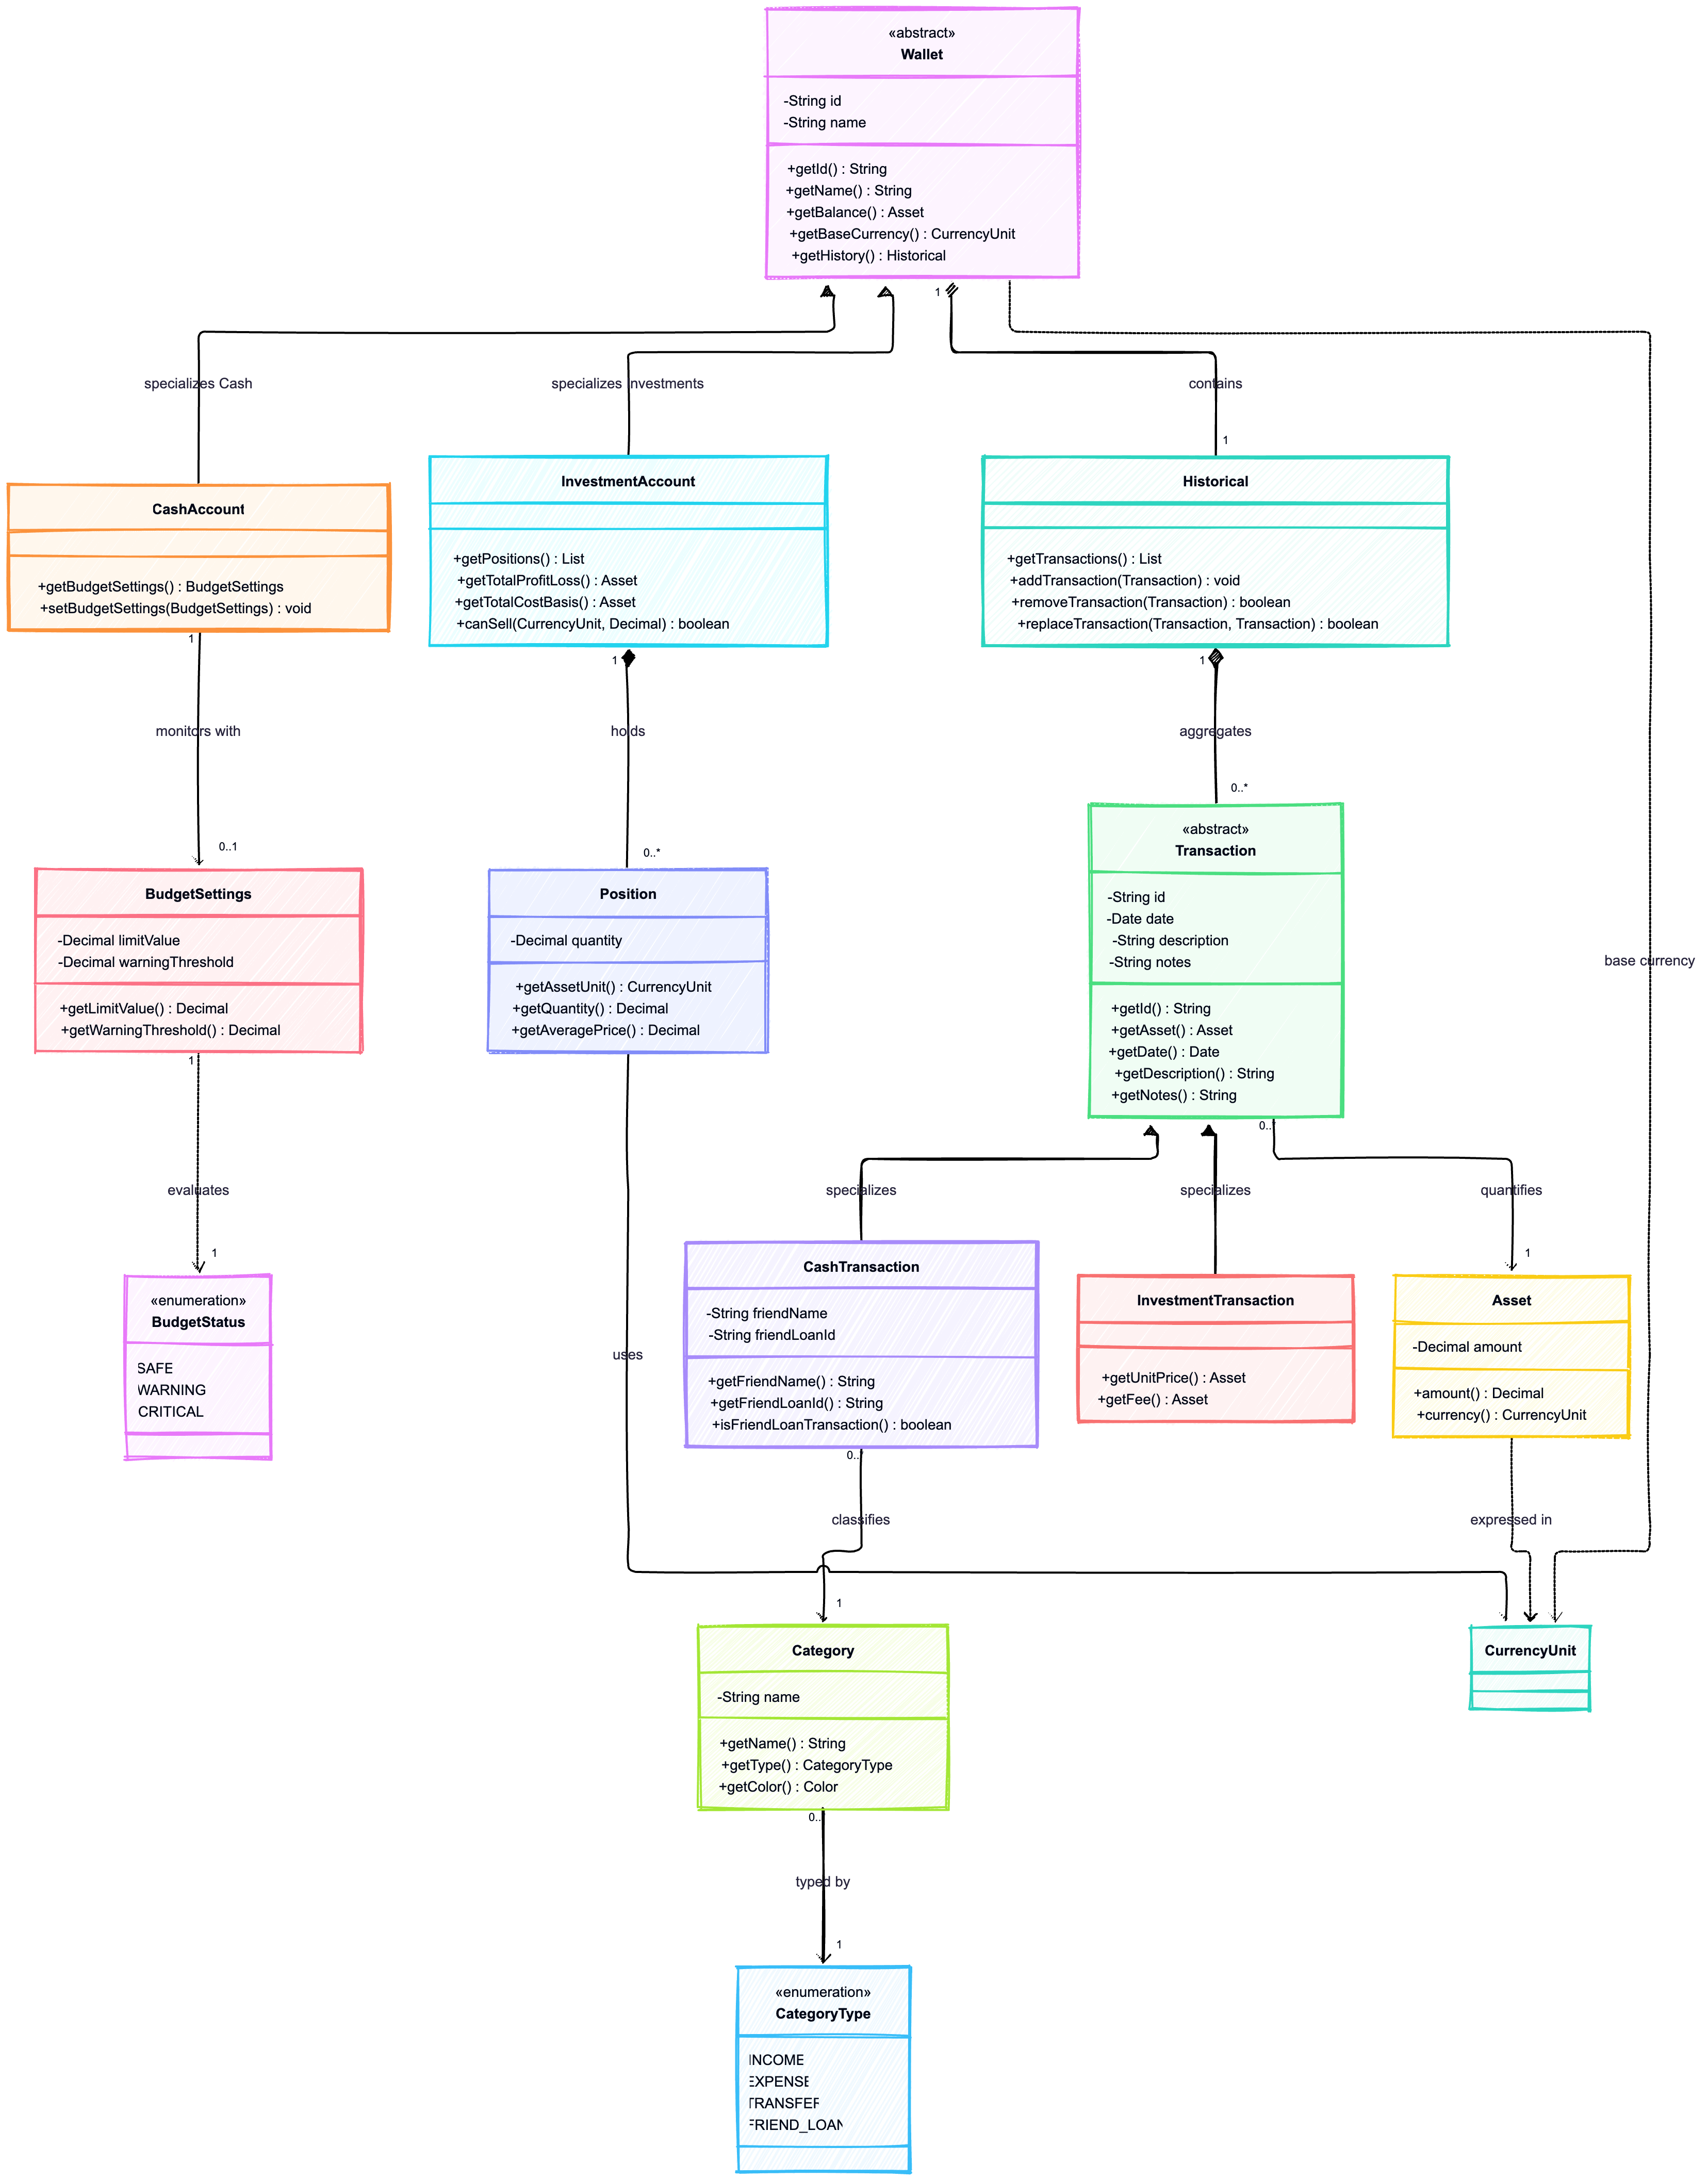
\includegraphics[width=\linewidth,height=0.85\textheight,keepaspectratio]{img/uml-dominio-1.png}
    \caption{Schema UML del dominio (Parte 1): conti, storico transazioni, posizioni e gestione del budget.}
    \label{fig:dominio-conti}
  \end{figure}

  \clearpage

  \begin{figure}[p]
    \centering
    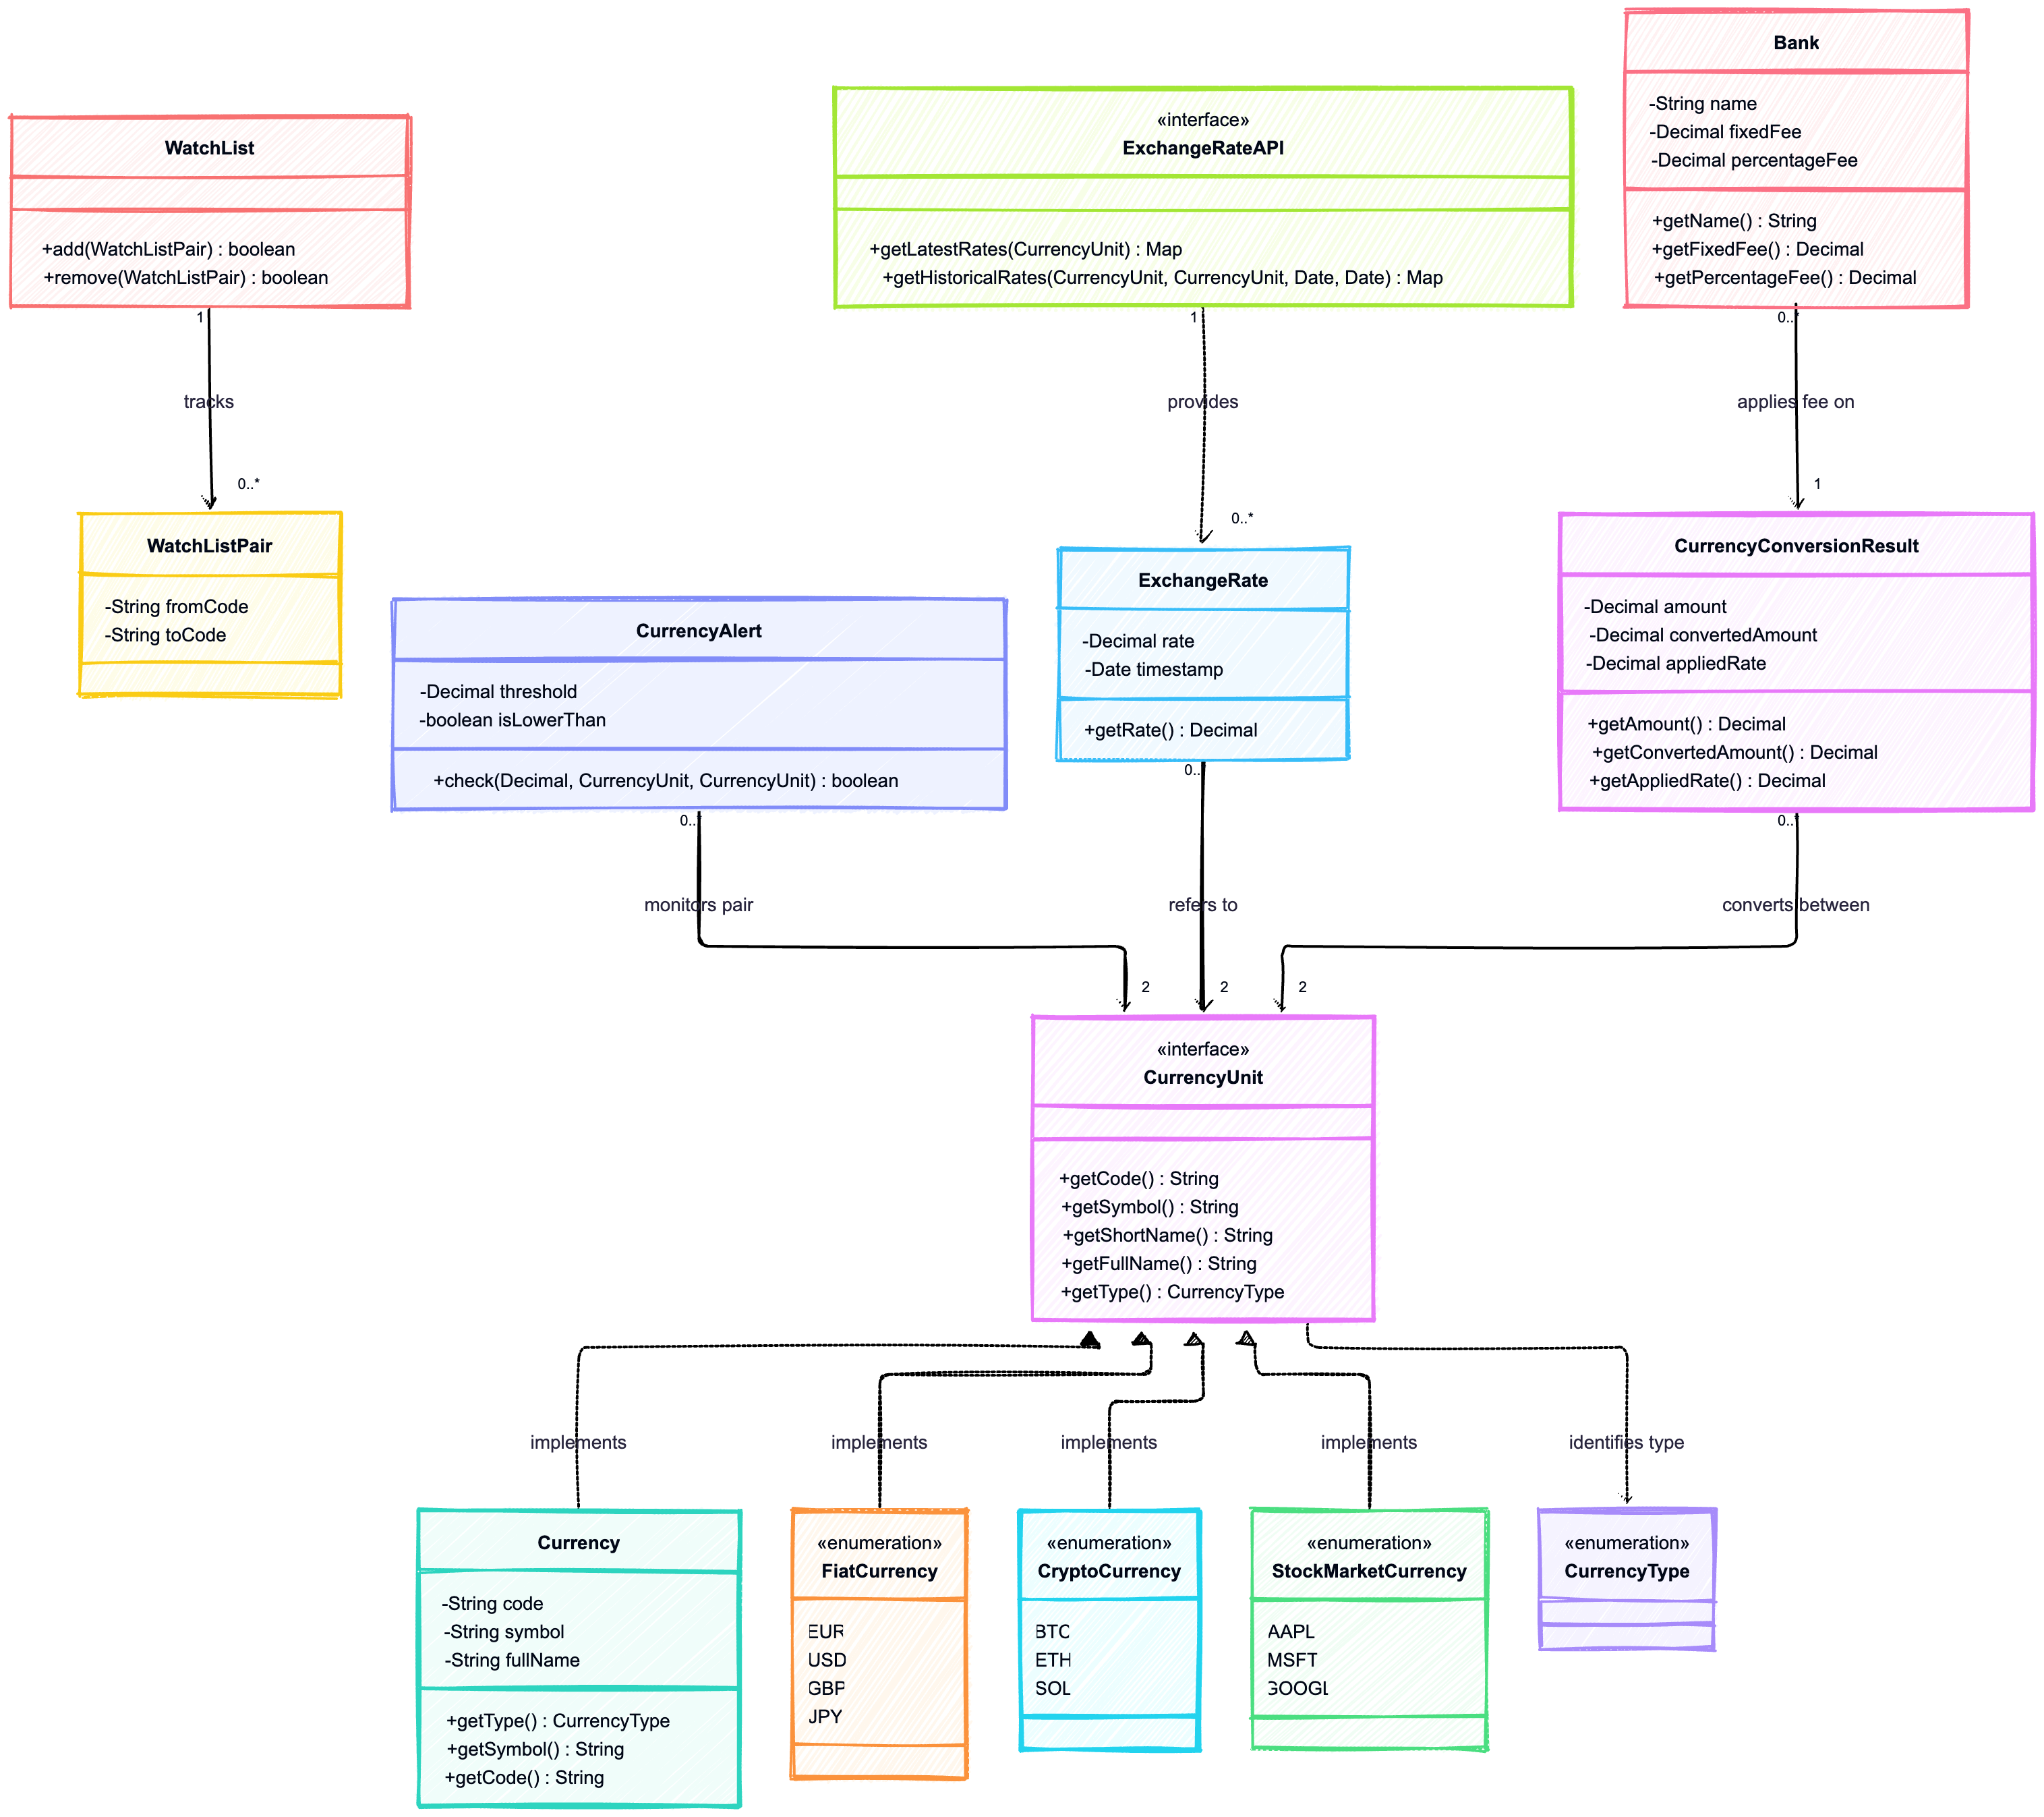
\includegraphics[width=\linewidth,height=0.85\textheight,keepaspectratio]{img/uml-dominio-2.png}
    \caption{Schema UML del dominio (Parte 2): mercati, tassi di cambio, watchlist, banche e conversioni valutarie.}
    \label{fig:dominio-mercato}
  \end{figure}
\end{landscape}

\clearpage

\subsection*{Aspetti critici}

Alcuni aspetti del problema sono particolarmente impegnativi.
\begin{itemize}
  \item \textbf{Valute eterogenee}. Euro, bitcoin e azioni hanno precisioni molto diverse e i loro prezzi
    provengono da fonti diverse. Non esiste un tasso diretto per ogni coppia di valute (ad esempio tra
    un'azione e una criptovaluta), e i tassi cambiano continuamente.
  \item \textbf{Valore degli investimenti}. Il saldo di un conto di liquidità dipende solo dalla sua
    storia; il valore di un conto di investimento dipende anche dal prezzo di mercato del momento. Con più
    acquisti a prezzi diversi e vendite parziali, il prezzo medio di carico e la distinzione tra profitto
    realizzato e non realizzato richiedono regole di calcolo precise.
  \item \textbf{Operazioni su più conti}. Un acquisto pagato con un conto di liquidità modifica due conti
    di tipo diverso, eventualmente in valute diverse; il pagamento può anche avvenire con una stablecoin
    dello stesso conto.
  \item \textbf{Correzioni nel passato}. Correggere o eliminare un movimento già registrato cambia tutti i
    saldi e le statistiche che ne dipendono.
  \item \textbf{Andamento nel tempo}. Per mostrare l'andamento di un conto di investimento il suo valore
    va registrato nel tempo, anche quando l'utente non fa nessuna operazione.
  \item \textbf{Fonti di prezzo esterne}. I servizi di quotazione gratuiti hanno limiti sul numero di
    richieste e possono non rispondere, mentre l'applicazione deve restare utilizzabile.
\end{itemize}

Alcune funzionalità sono state lasciate fuori da questa versione: l'importazione automatica dei movimenti
dalle banche, le quotazioni in tempo reale, il calcolo delle tasse sui guadagni e la gestione di più
utenti. Le valute supportate sono un elenco predefinito, che può essere esteso ma non dall'interfaccia
dell'applicazione.

\chapter{Design}

In questo capitolo vengono descritte la struttura architetturale complessiva di UniBodget e le strategie di progettazione dettagliate adottate da \textbf{Arianna Palmucci} per la risoluzione dei problemi cardine a lei assegnati.

\section{Architettura}
\enlargethispage{3\baselineskip}
Il sistema adotta il pattern architetturale \textbf{Model-View-Controller (MVC)} integrato con una struttura reattiva basata su un bus di messaggi disaccoppiato (\texttt{MessageBus}), come sintetizzato nello schema di Figura~\ref{fig:architecture}. Tale impostazione garantisce il completo isolamento della logica applicativa rispetto al toolkit grafico (JavaFX 21).

\subsection*{Ruoli dei Componenti Architetturali}
\begin{itemize}
    \item \textbf{Model:} Incapsula lo stato persistente dell'applicazione, le regole di business contabili, gli algoritmi di conversione e i meccanismi di serializzazione. Il modello è puro: non contiene alcuna dipendenza verso librerie grafiche (\texttt{javafx.*}) ed è completamente testabile in ambienti headless.
    \item \textbf{Controller:} Intercetta i comandi dell'utente inviati dalla vista, coordina le invocazioni verso i servizi del modello e trasforma le entità di business in strutture dati di presentazione (view models e records immutabili) consumabili dalla GUI.
    \item \textbf{View:} Costruita interamente in JavaFX attraverso una combinazione di file FXML e viste programmatiche modulari. Si occupa unicamente del rendering grafico e dell'ascolto delle interazioni utente, delegando ogni logica decisionale al rispettivo controller.
\end{itemize}

\subsection*{Disaccoppiamento View-Controller}
Il disaccoppiamento è garantito dall'adozione del principio di inversione delle dipendenze:
\begin{itemize}
    \item I controller non detengono riferimenti a classi di layout o nodi visivi specifici (non manipolano \texttt{TextField}, \texttt{TableView} o controlli FXML), ma operano tramite interfacce di callback (\texttt{Consumer}, \texttt{Runnable}, \texttt{Supplier}).
    \item Nel modulo di conversione (\texttt{CurrencyConverterModule}), l'intera vista è esposta verso la shell principale come un generico nodo radice \texttt{Parent}, rendendo la composizione dell'interfaccia totalmente agnostica rispetto ai widget interni.
    \item La sostituzione completa del framework grafico (ad esempio verso Swing o una web UI) richiederebbe unicamente la riscrittura del layer View, lasciando immutati sia il Controller sia l'intero Model.
\end{itemize}

\begin{landscape}
  \begin{figure}[p]
    \centering
    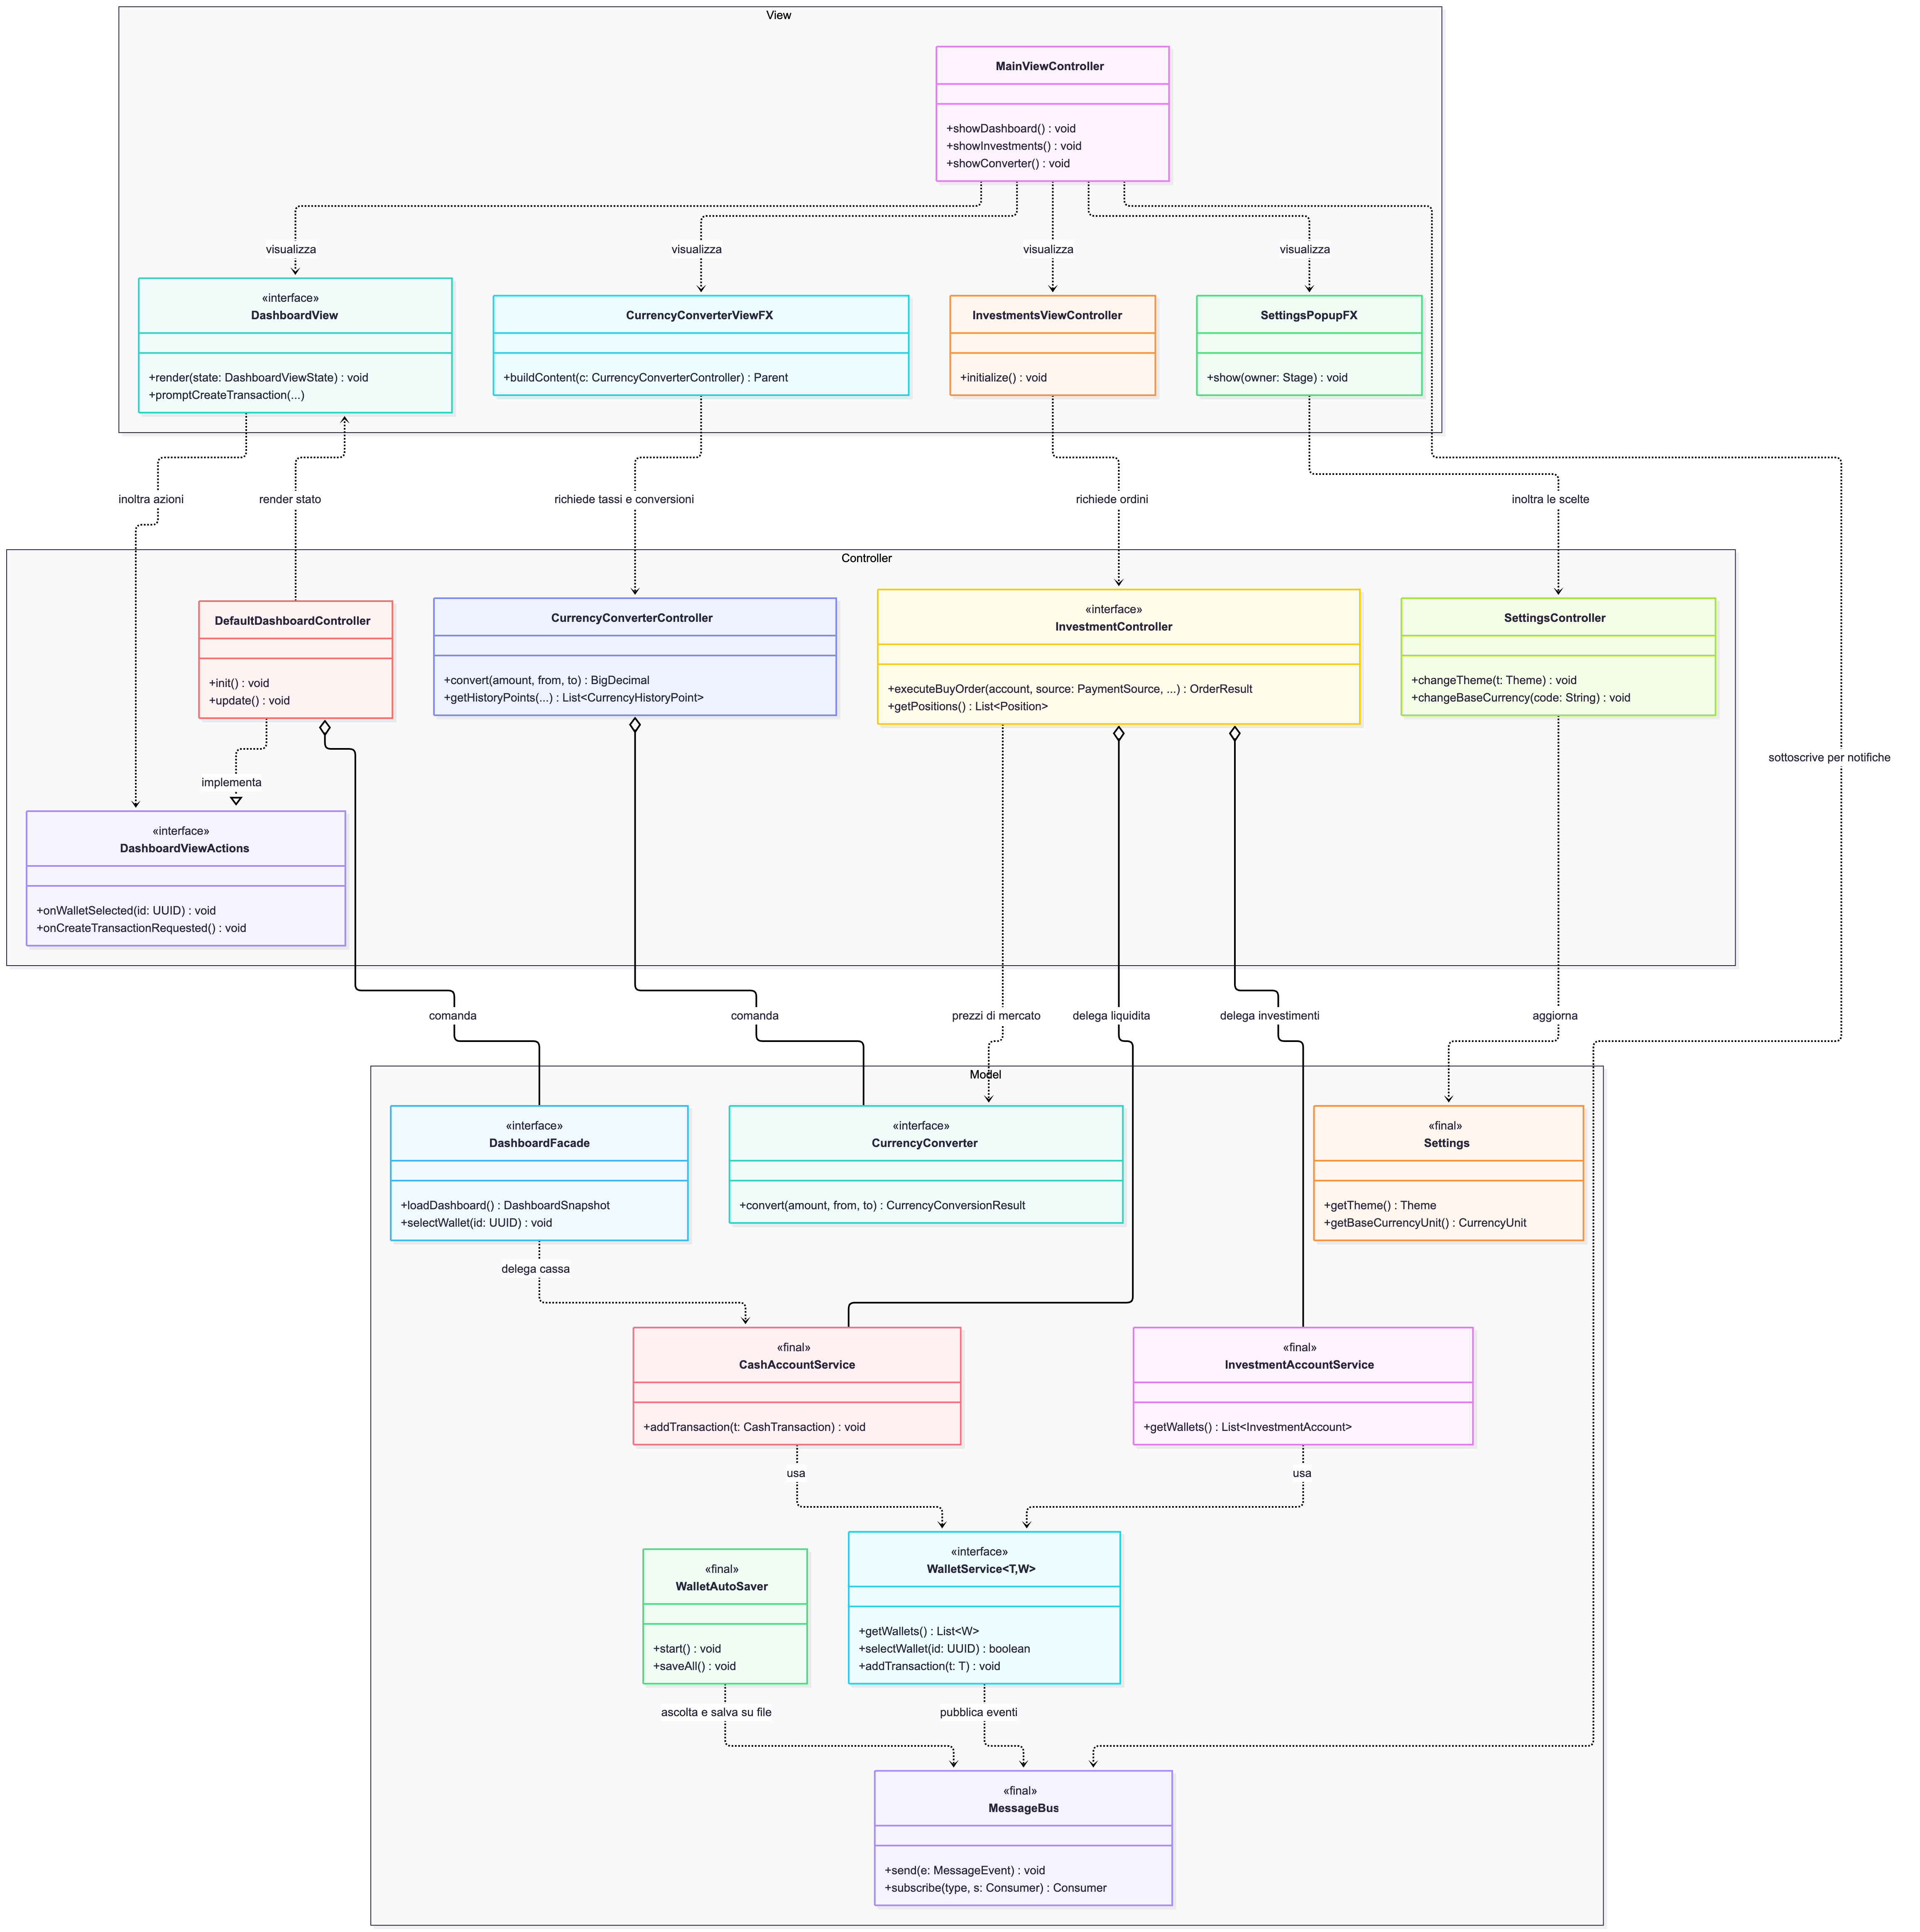
\includegraphics[width=\linewidth,height=0.85\textheight,keepaspectratio]{img/uml-architettura.png}
    \caption{Rappresentazione ad alto livello dell'architettura MVC e del MessageBus disaccoppiato.}
    \label{fig:architecture}
  \end{figure}
\end{landscape}

% ============================================================================
% 2.2 DESIGN DETTAGLIATO (ARIANNA PALMUCCI)
% ============================================================================
\section{Design Dettagliato (Arianna Palmucci)}

In questa sezione vengono dettagliati i cinque principali problemi di progettazione affrontati e risolti, con l'analisi delle alternative scartate, la descrizione delle soluzioni e la reificazione dei design pattern adottati.

% ----------------------------------------------------------------------------
\subsection{Sistema Polimorfico delle Valute e Motore di Conversione}

\subsubsection*{1. Descrizione del problema}
L'applicazione necessita di operare con classi di attività finanziarie eterogenee (valute a corso legale, criptovalute e titoli azionari). Tali attività presentano caratteristiche intrinseche profondamente disomogenee:
\begin{itemize}
    \item Le valute fiat operano con convenzioni a 2 o 4 decimali e identificatori ISO standard (EUR, USD, GBP, ecc.).
    \item Le criptovalute presentano frazionabilità elevatissima (fino a 8--18 decimali) e richiedono identificatori specifici per le API di quotazione (es. \texttt{apiId} come \texttt{"bitcoin"}).
    \item I titoli azionari operano con ticker di borsa (es. \texttt{AAPL}, \texttt{GOOGL}) e mercati di riferimento regolamentati.
\end{itemize}
Inoltre, il calcolo della conversione tra due qualsiasi valute deve essere flessibile, estendibile e svincolato dall'implementazione specifica della sorgente dei tassi.

\subsubsection*{2. Soluzione proposta e alternative}
\begin{itemize}
    \item \textbf{Alternativa scartata (Classe monolitica o enum universale):} Raggruppare tutte le tipologie in un'unica enum con campi facoltativi avrebbe violato i principi \emph{Open/Closed} (OCP) e \emph{Single Responsibility} (SRP), obbligando a modificare codice esistente per aggiungere nuove valute o mercati.
    \item \textbf{Soluzione adottata:} Definizione dell'interfaccia comune \texttt{CurrencyUnit}, implementata in modo polimorfico da enum fortemente tipizzate: \texttt{FiatCurrency}, \texttt{CryptoCurrency} e \texttt{StockMarketCurrency}, oltre alla classe aperta \texttt{Currency} per asset personalizzati. Per l'esecuzione dei cambi è stata definita l'interfaccia \texttt{CurrencyConverter}, la cui implementazione principale \texttt{BasicCurrencyConverter} esegue calcoli rigorosi su \texttt{BigDecimal} con rounding bancario (\texttt{RoundingMode.HALF\_UP}), incapsulando il risultato nel record immutabile \texttt{CurrencyConversionResult}.
\end{itemize}

\subsubsection*{3. Schema UML e Interazioni}
La gerarchia delle valute e il motore di conversione sono strutturati come segue:
\begin{itemize}
    \item \texttt{CurrencyUnit} (interfaccia radice): espone \texttt{getCode()}, \texttt{getSymbol()}, \texttt{getShortName()}, \texttt{getFullName()}, \texttt{getType()}.
    \item \texttt{FiatCurrency}, \texttt{CryptoCurrency}, \texttt{StockMarketCurrency}, \texttt{Currency}: implementano \texttt{CurrencyUnit}.
    \item \texttt{CurrencyConverter} (interfaccia): definisce \texttt{convert(amount, from, to)}.
    \item \texttt{BasicCurrencyConverter}: implementa \texttt{CurrencyConverter} delegando a \texttt{UniversalPriceService} per il recupero delle quotazioni relative al dollaro USD e calcolando il tasso cross applicato.
\end{itemize}

\subsubsection*{4. Pattern utilizzati e reificazione}
\begin{itemize}
    \item \textbf{Strategy Pattern:} L'interfaccia \texttt{CurrencyConverter} rappresenta la \emph{Strategy} astratta per il calcolo delle conversioni. \texttt{BasicCurrencyConverter} costituisce la \emph{Concrete Strategy} che esegue la triangolazione ponderata sui tassi correnti. Il client (\texttt{CurrencyConverterController} e \texttt{ConverterWidgetFX}) opera esclusivamente contro l'interfaccia, consentendo la sostituzione trasparente dell'algoritmo di conversione (es. per collaudo o con commissioni istituzionali).
    \item \textbf{Adapter Pattern:} I dati eterogenei restituiti dai provider remoti (payload JSON di formati differenti) vengono normalizzati attraverso \texttt{ExchangeRateAPIClient} e \texttt{UniversalPriceService}, che fungono da \emph{Adapter} verso le strutture di dominio interne.
\end{itemize}

\begin{figure}[H]
    \centering
    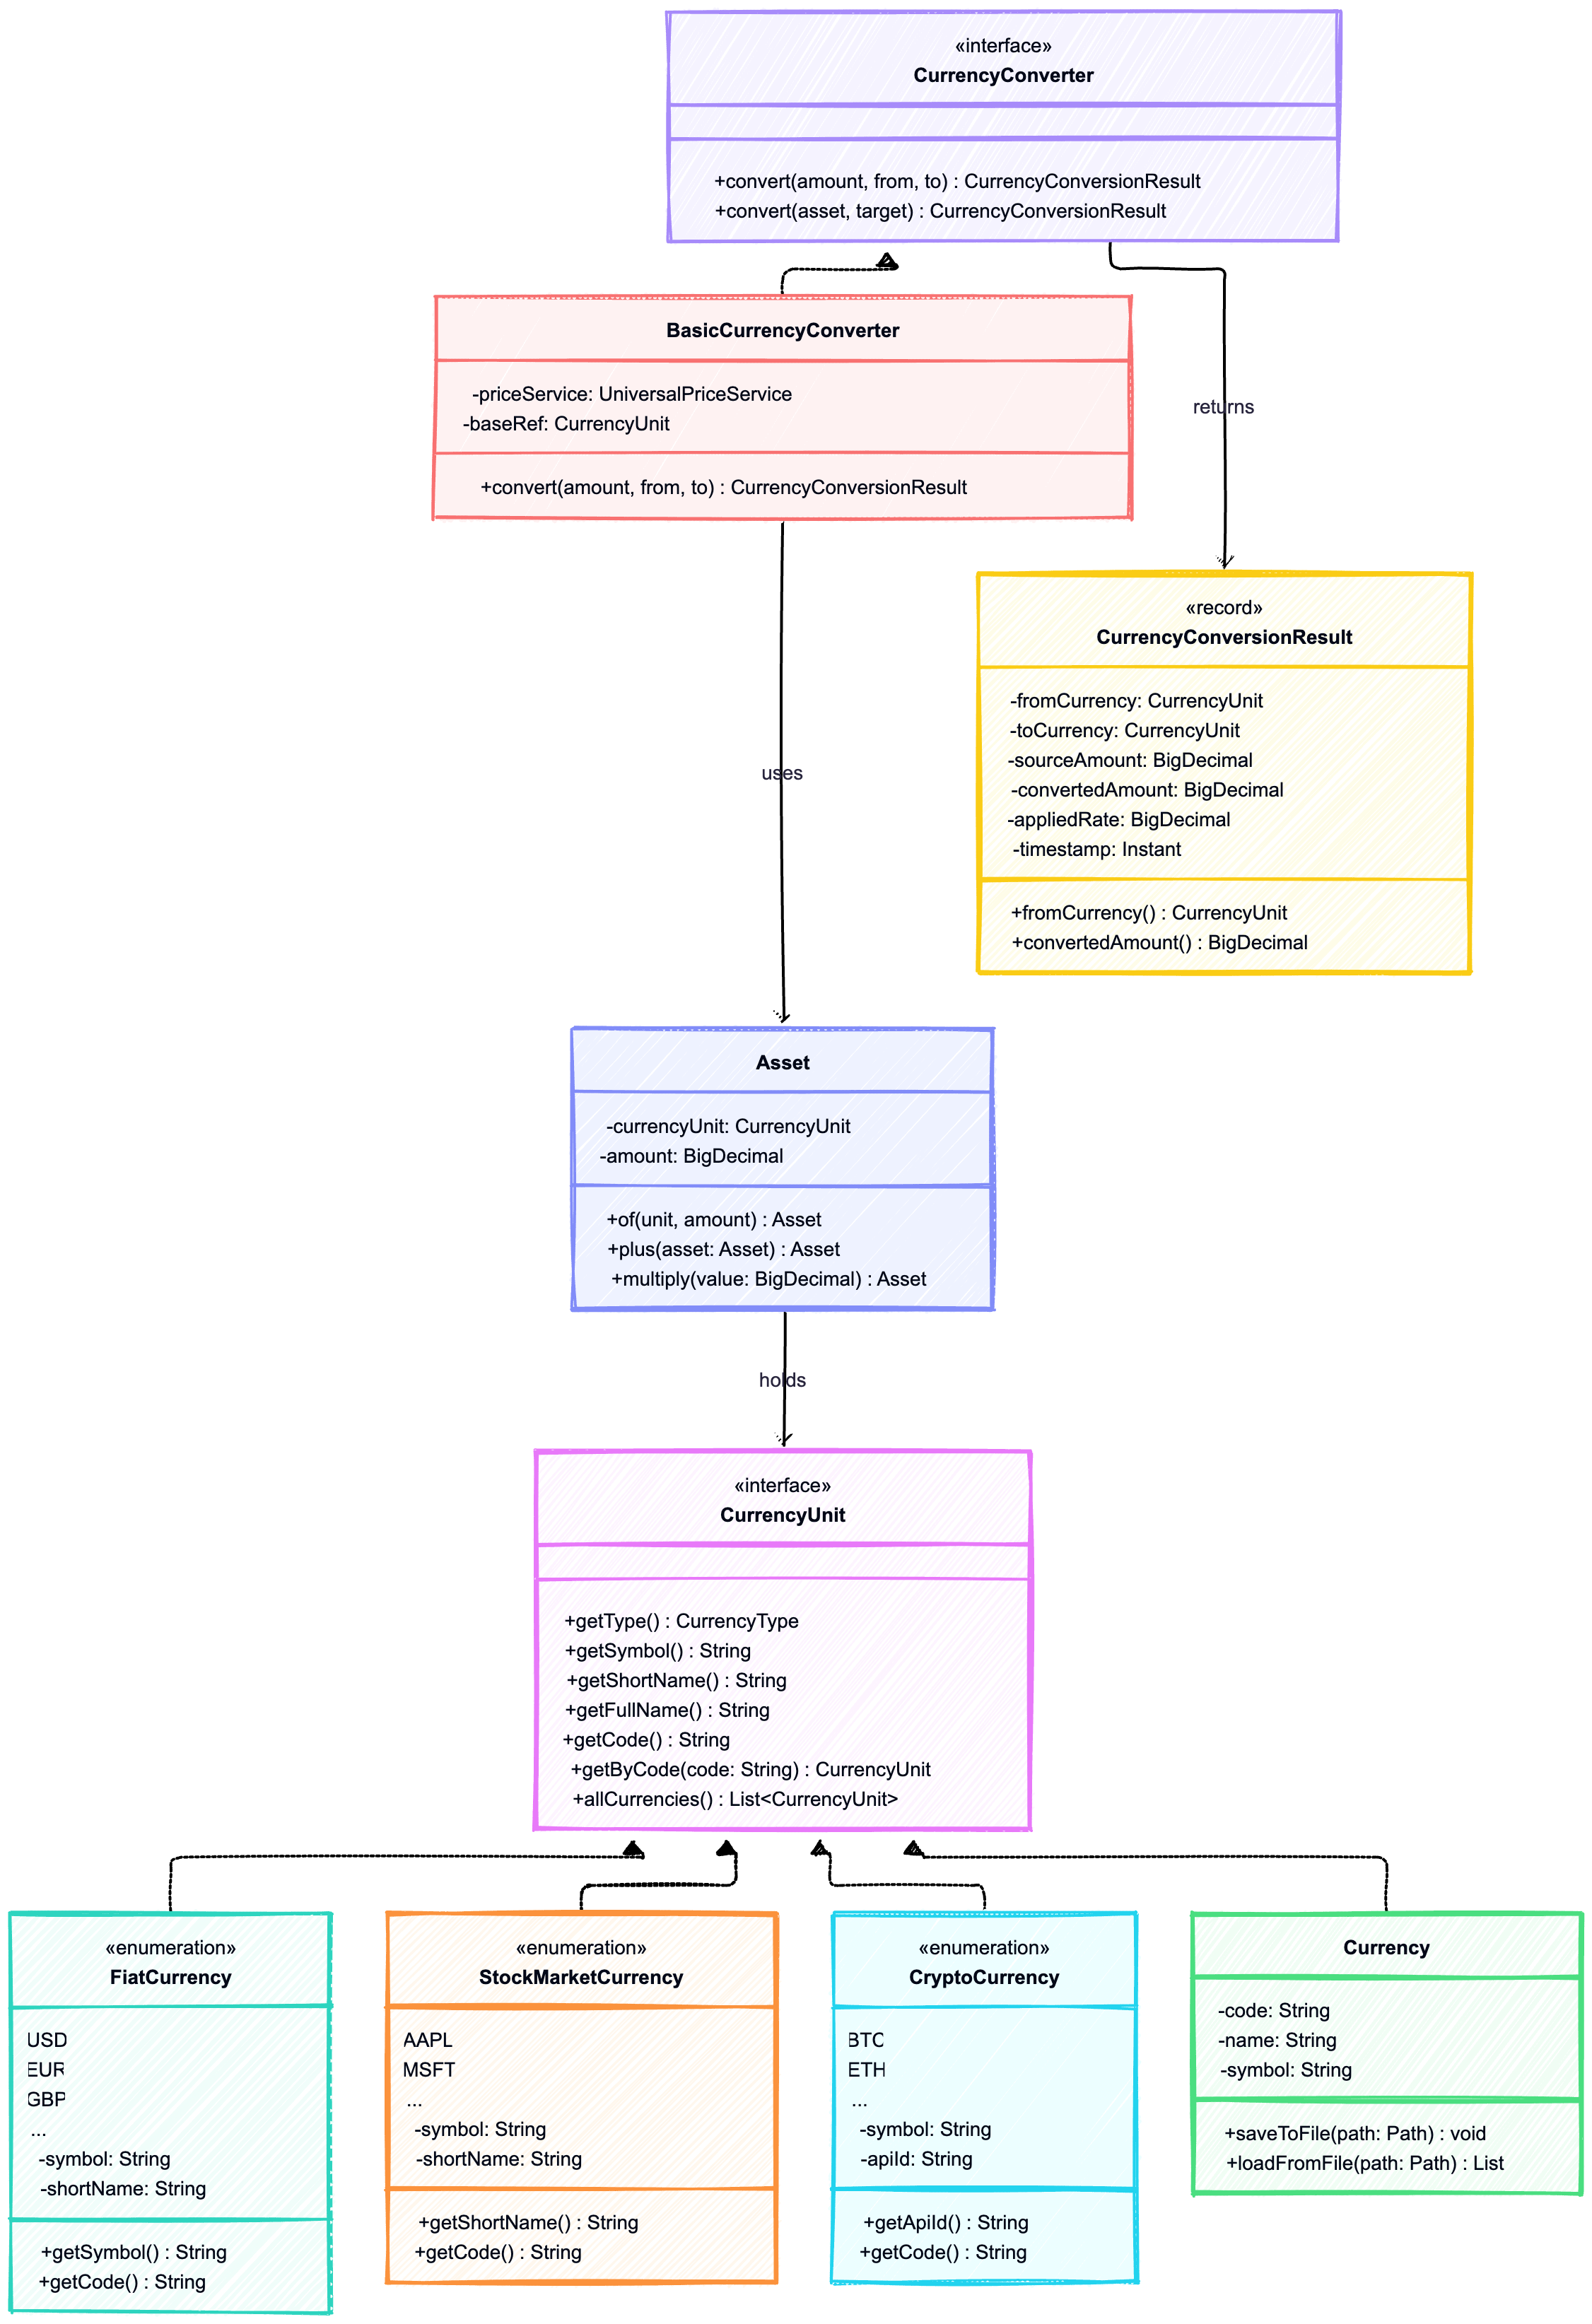
\includegraphics[width=0.95\textwidth,keepaspectratio]{img/uml-currency.png}
    \caption{Il diagramma illusta gerarchia polimorfica di \texttt{CurrencyUnit}, \texttt{Asset} e motore di conversione.}
    \label{fig:currency-hierarchy}
\end{figure}

% ----------------------------------------------------------------------------
\subsection{Architettura dei Provider di Cambio con Caching Resiliente}

\subsubsection*{1. Descrizione del problema}
I servizi web esterni che forniscono le quotazioni di mercato delle diverse classi di attività (open.er-api.com per le valute legali fiat, CoinGecko v3 per le criptovalute, Alpha Vantage per i titoli azionari di borsa) impongono vincoli operativi e architetturali stringenti:
\begin{enumerate}
    \item \textbf{Rate Limiting e Quote d'Uso Rigide:} I piani API gratuiti applicano soglie restrittive (es. 25--100 chiamate giornaliere su Alpha Vantage, 10--30 richieste al minuto su CoinGecko). Il superamento di tali limiti comporta il blocco temporaneo dell'indirizzo IP con codici di errore HTTP.
    \item \textbf{Latenza e Rischio di Blocco della GUI:} Le chiamate HTTP su rete pubblica introducono tempi di risposta variabili (da centinaia di millisecondi a diversi secondi in caso di congestione). L'esecuzione sincrona non mediata sul thread applicativo JavaFX congelerebbe l'interfaccia.
    \item \textbf{Resilienza Offline e Tolleranza ai Guasti:} L'applicazione deve garantire la piena continuità operativa anche in caso di assenza temporanea di connettività Internet, timeout di rete o manutenzione dei server remoti, senza perdere dati e senza generare crash inattesi.
\end{enumerate}

\subsubsection*{2. Soluzione proposta e alternative}
\begin{itemize}
    \item \textbf{Alternativa scartata A (Chiamate dirette sincrone senza memorizzazione):} Interrogare direttamente l'endpoint REST ad ogni conversione o render grafico provocherebbe l'esaurimento delle quote API in pochi secondi di utilizzo e un'esperienza utente inaccettabile in caso di latenza.
    \item \textbf{Alternativa scartata B (Thread demone di polling periodico continuo):} Interrogare ciclicamente i server remoti in background consumerebbe inutilmente traffico dati e risorse computazionali anche quando l'utente non sta consultando il convertitore o il portafoglio.
    \item \textbf{Soluzione architetturale adottata:} Introduzione di un'architettura multilivello basata su:
    \begin{enumerate}
        \item \emph{Cache in memoria ad accesso immediato controllata da Time-To-Live (TTL):} Le risposte valide delle API vengono memorizzate associando un timestamp di aggiornamento (\texttt{Instant}). Ogni richiesta successiva pervenuta entro la finestra di validità viene servita in tempo costante ($O(1)$) dalla memoria, senza alcun traffico di rete;
        \item \emph{Graceful Degradation e Provider Deterministico di Fallback:} In caso di errore HTTP, timeout o modalità offline, il sistema ricorre all'ultimo tasso valido memorizzato; qualora non vi sia alcuna quotazione pregressa (es. primo avvio offline o test automatizzati), interviene il componente \texttt{MockExchangeRateAPI}, che genera tassi realistici e riproducibili azzerando il rischio di interruzione del servizio.
    \end{enumerate}
\end{itemize}

\subsubsection*{3. Schema UML e Interazioni}
L'interfaccia \texttt{ExchangeRateAPI} espone i metodi \texttt{getLatestRates(base)} e \texttt{getHistoricalRates(base, target, from, to)}.
\texttt{ExchangeRateAPIImpl} implementa tale contratto mantenendo una mappa \texttt{cachedRates} associata a un timestamp \texttt{Instant lastUpdate}. Se la richiesta perviene entro la finestra di validità della cache, i dati vengono restituiti istantaneamente; in caso contrario, viene effettuata la chiamata HTTP aggiornando la cache solo a fronte di una risposta valida (HTTP 200). Parallelamente, \texttt{UniversalPriceService} coordina i provider dedicati per le diverse classi di asset, delegando a \texttt{PriceProvider} per quotazioni crittografiche e azionarie:

\begin{figure}[H]
    \centering
    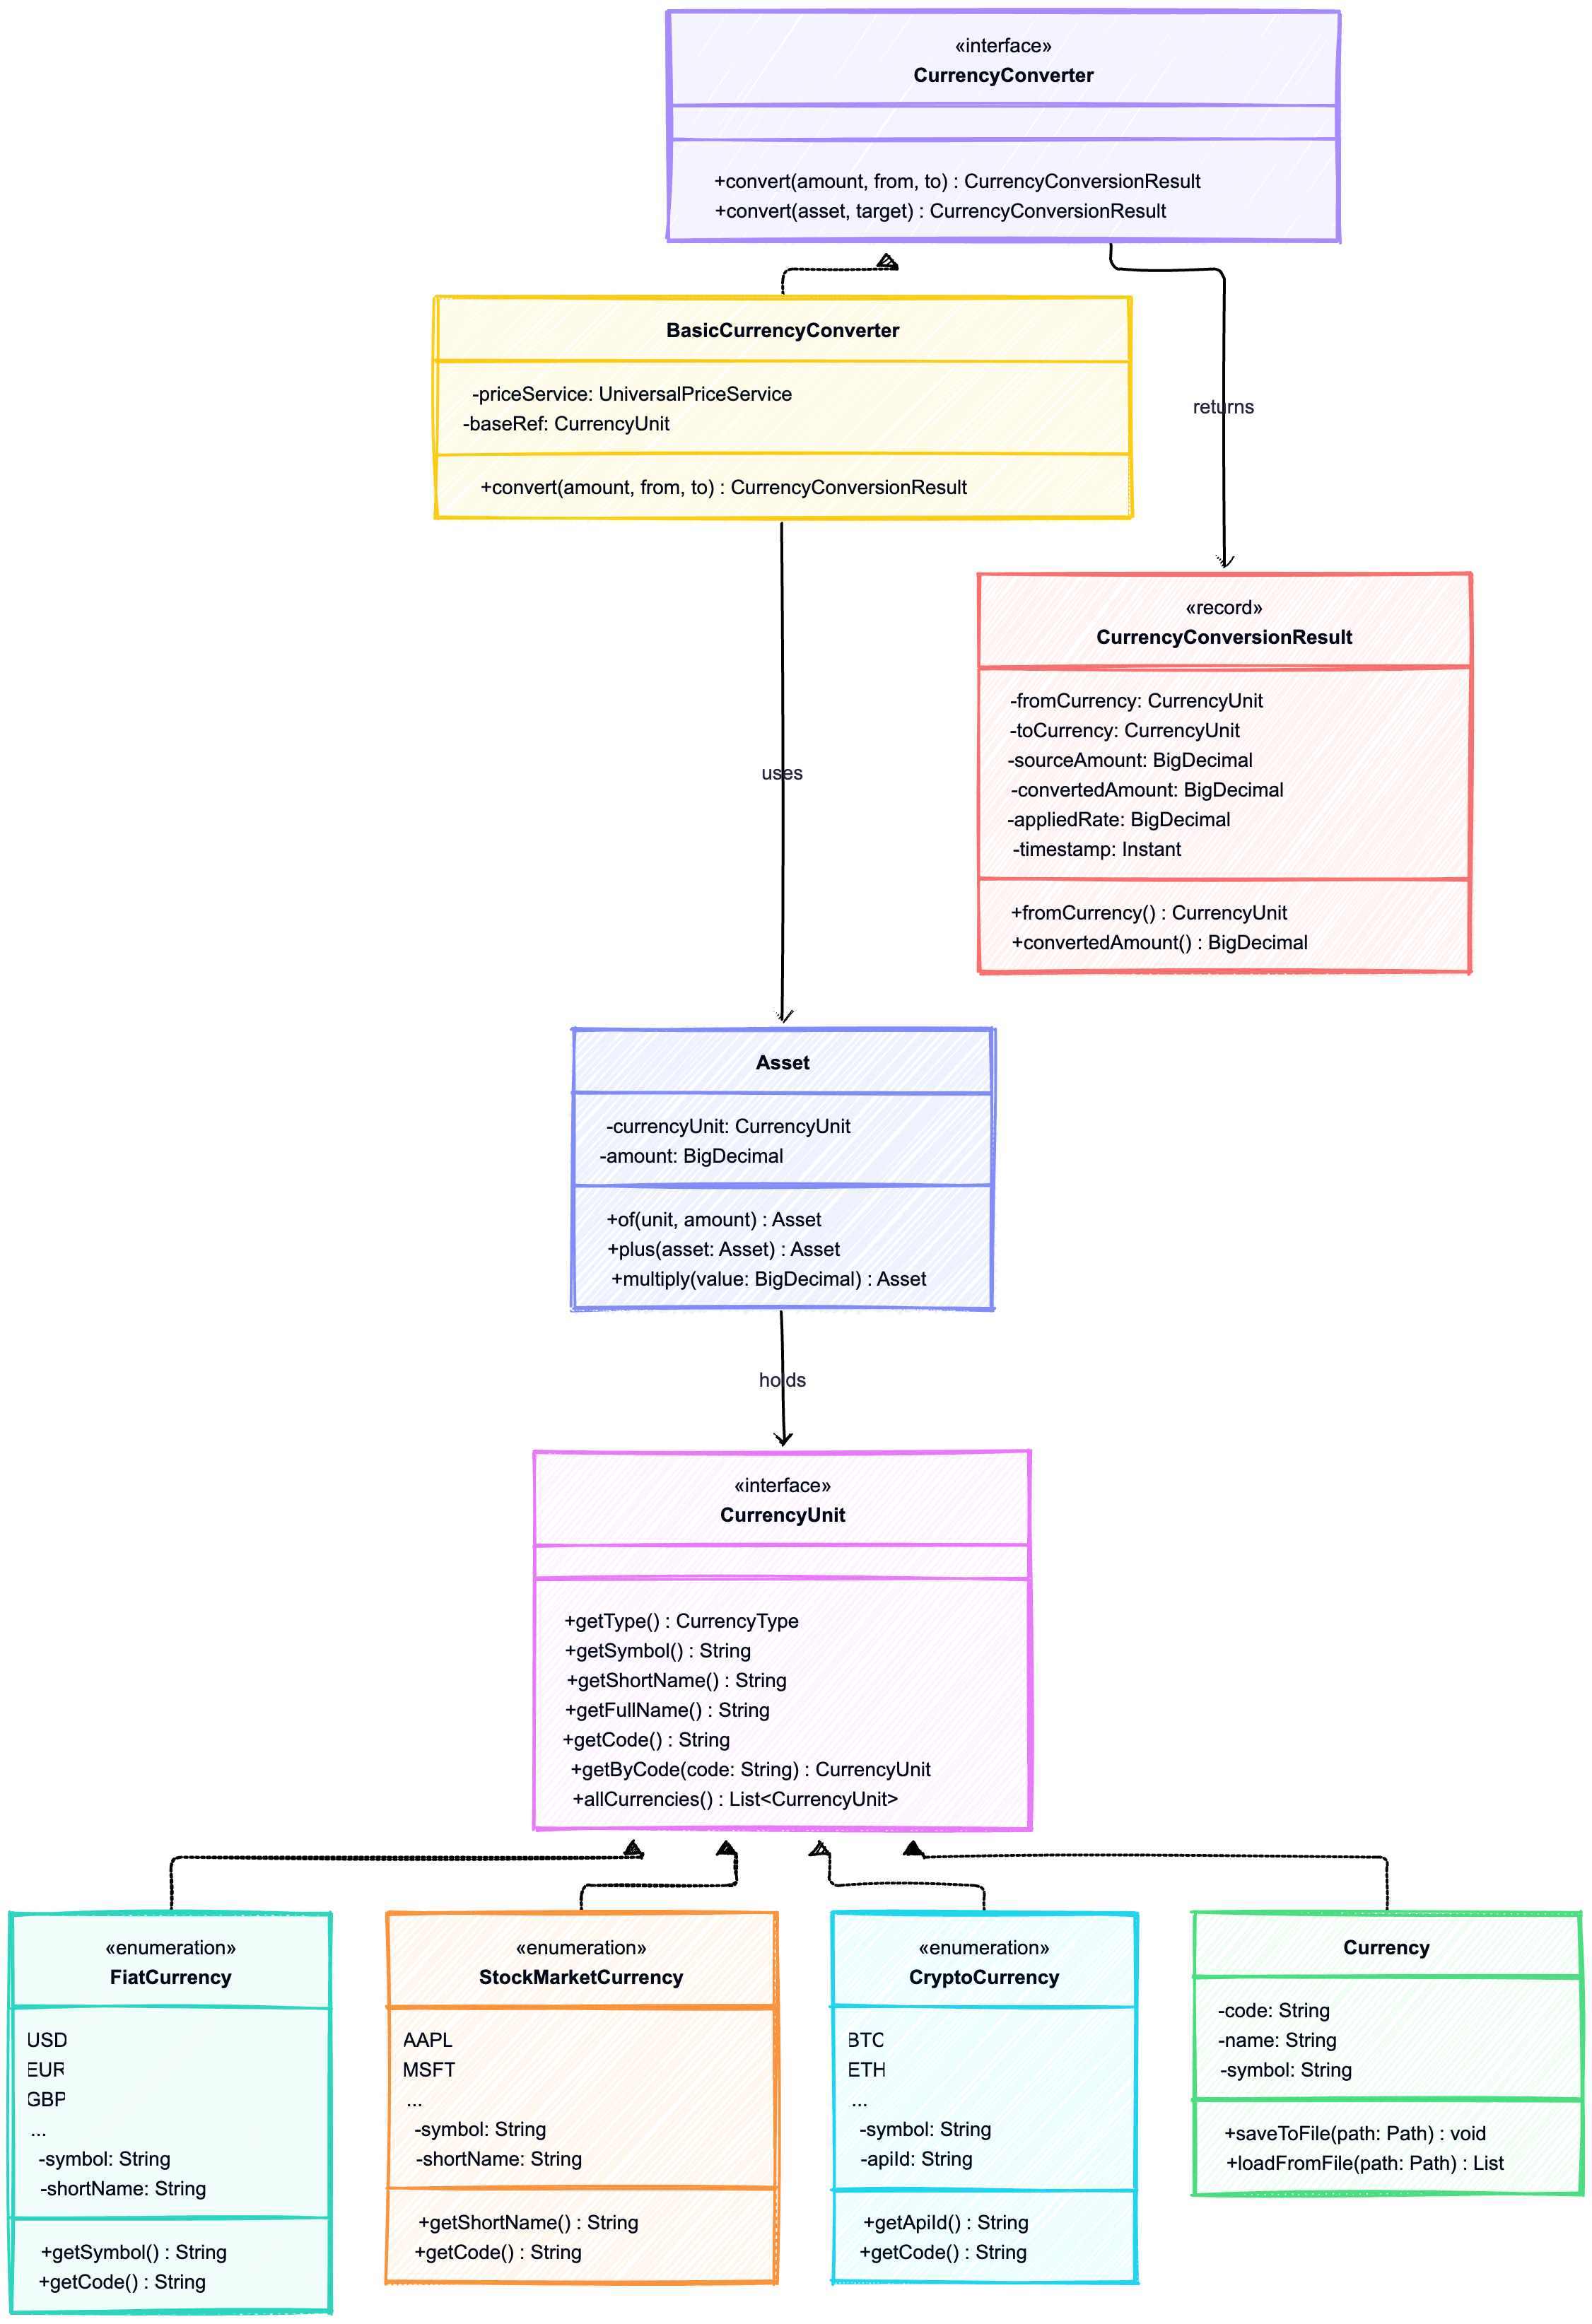
\includegraphics[
        width=0.95\textwidth,
        keepaspectratio
    ]{img/uml-conversion.png}
    \caption{Diagramma delle classi: gerarchia polimorfica di \texttt{CurrencyUnit}, \texttt{Asset} e motore di conversione.}
    \label{fig:currency-conversion}
\end{figure}

\subsubsection*{4. Pattern utilizzati e reificazione}
\begin{itemize}
    \item \textbf{Cache Proxy Pattern:} \texttt{ExchangeRateAPIImpl} controlla e protegge l'accesso alla risorsa remota costosa (chiamate di rete su protocollo HTTP), intercettando le richieste e soddisfacendole dalla cache interna ogni qualvolta i dati siano ancora validi.
    \item \textbf{Null Object / Fallback Strategy Pattern:} \texttt{MockExchangeRateAPI} offre un'implementazione autonoma e affidabile dei contratti di mercato, garantendo la totale continuità operativa del sistema e la determinazione nei test automatici.
\end{itemize}

% ----------------------------------------------------------------------------
\subsection{Monitoraggio dei Tassi, Allerte di Mercato e Watchlist Reattiva}

\subsubsection*{1. Descrizione del problema}
Un cruscotto finanziario completo richiede strumenti operativi di monitoraggio continuo:
\begin{enumerate}
    \item \textbf{Tracciamento di Coppie Valutarie Dinamiche (\emph{Watchlist}):} L'utente deve poter fissare un insieme personalizzato di coppie di scambio preferite per consultarne il tasso in tempo reale senza dover reimpostare ogni volta i menu di conversione;
    \item \textbf{Allerte di Prezzo Reattive con Soglie Limite (\emph{Alerts}):} L'utente deve poter definire soglie di cambio critiche (es. notificare se $1\text{ EUR} > 1.10\text{ USD}$ oppure se $1\text{ BTC} < 60000\text{ USD}$), con direzione di attraversamento (\emph{ABOVE} o \emph{BELOW});
    \item \textbf{Preservazione del Disaccoppiamento MVC e Headless Testing:} La valutazione matematica delle condizioni di soglia non deve in alcun caso dipendere da primitive grafiche JavaFX (es. \texttt{javafx.scene.control.Alert}), preservando la rigorosa testabilità automatizzata.
\end{enumerate}

\subsubsection*{2. Soluzione proposta e alternative}
\begin{itemize}
    \item \textbf{Alternativa scartata A (Controlli grafici inseriti direttamente nel Model):} Invocare finestre di dialogo modali all'interno della logica contabile violerebbe il principio di singola responsabilità (SRP), impedirebbe l'esecuzione dei test JUnit in ambienti headless e creerebbe dipendenze circolari tra Model e View.
    \item \textbf{Alternativa scartata B (Valutazione cablata nei controller delle singole form):} Duplicare il controllo delle soglie all'interno di ciascun widget visivo causerebbe ridondanza di codice e inconsistenze qualora la medesima coppia sia visualizzata sia nel convertitore sia nella watchlist.
    \item \textbf{Soluzione adottata:} Architettura a responsabilità rigorosamente segregate:
    \begin{itemize}
        \item \texttt{CurrencyAlert}: record immutabile che incapsula la coppia valutaria, la soglia numerica e la direzione di allerta (\texttt{AlertDirection.ABOVE} o \texttt{BELOW});
        \item \texttt{CurrencyAlertService}: servizio puro del modello (privo di dipendenze da JavaFX) che custodisce l'elenco delle allerte attive ed espone il metodo funzionale \texttt{checkAlerts(rate, from, to)}, filtrando dichiarativamente tramite Stream le sole allerte che risultano effettivamente violate;
        \item \texttt{MarketAlertView}: componente specializzato del layer View che riceve le allerte violate dal servizio e pianifica l'apertura del dialogo modale d'allerta sul thread grafico;
        \item \texttt{WatchList}: componente di persistenza locale che mantiene un insieme unico (\texttt{Set<WatchlistPair>}) salvato atomicamente in formato JSON.
    \end{itemize}
\end{itemize}

\subsubsection*{3. Schema UML e Interazioni}
La separazione dei componenti per il monitoraggio reattivo dei mercati e per la gestione della watchlist è illustrata nel seguente diagramma:

\begin{figure}[H]
    \centering
    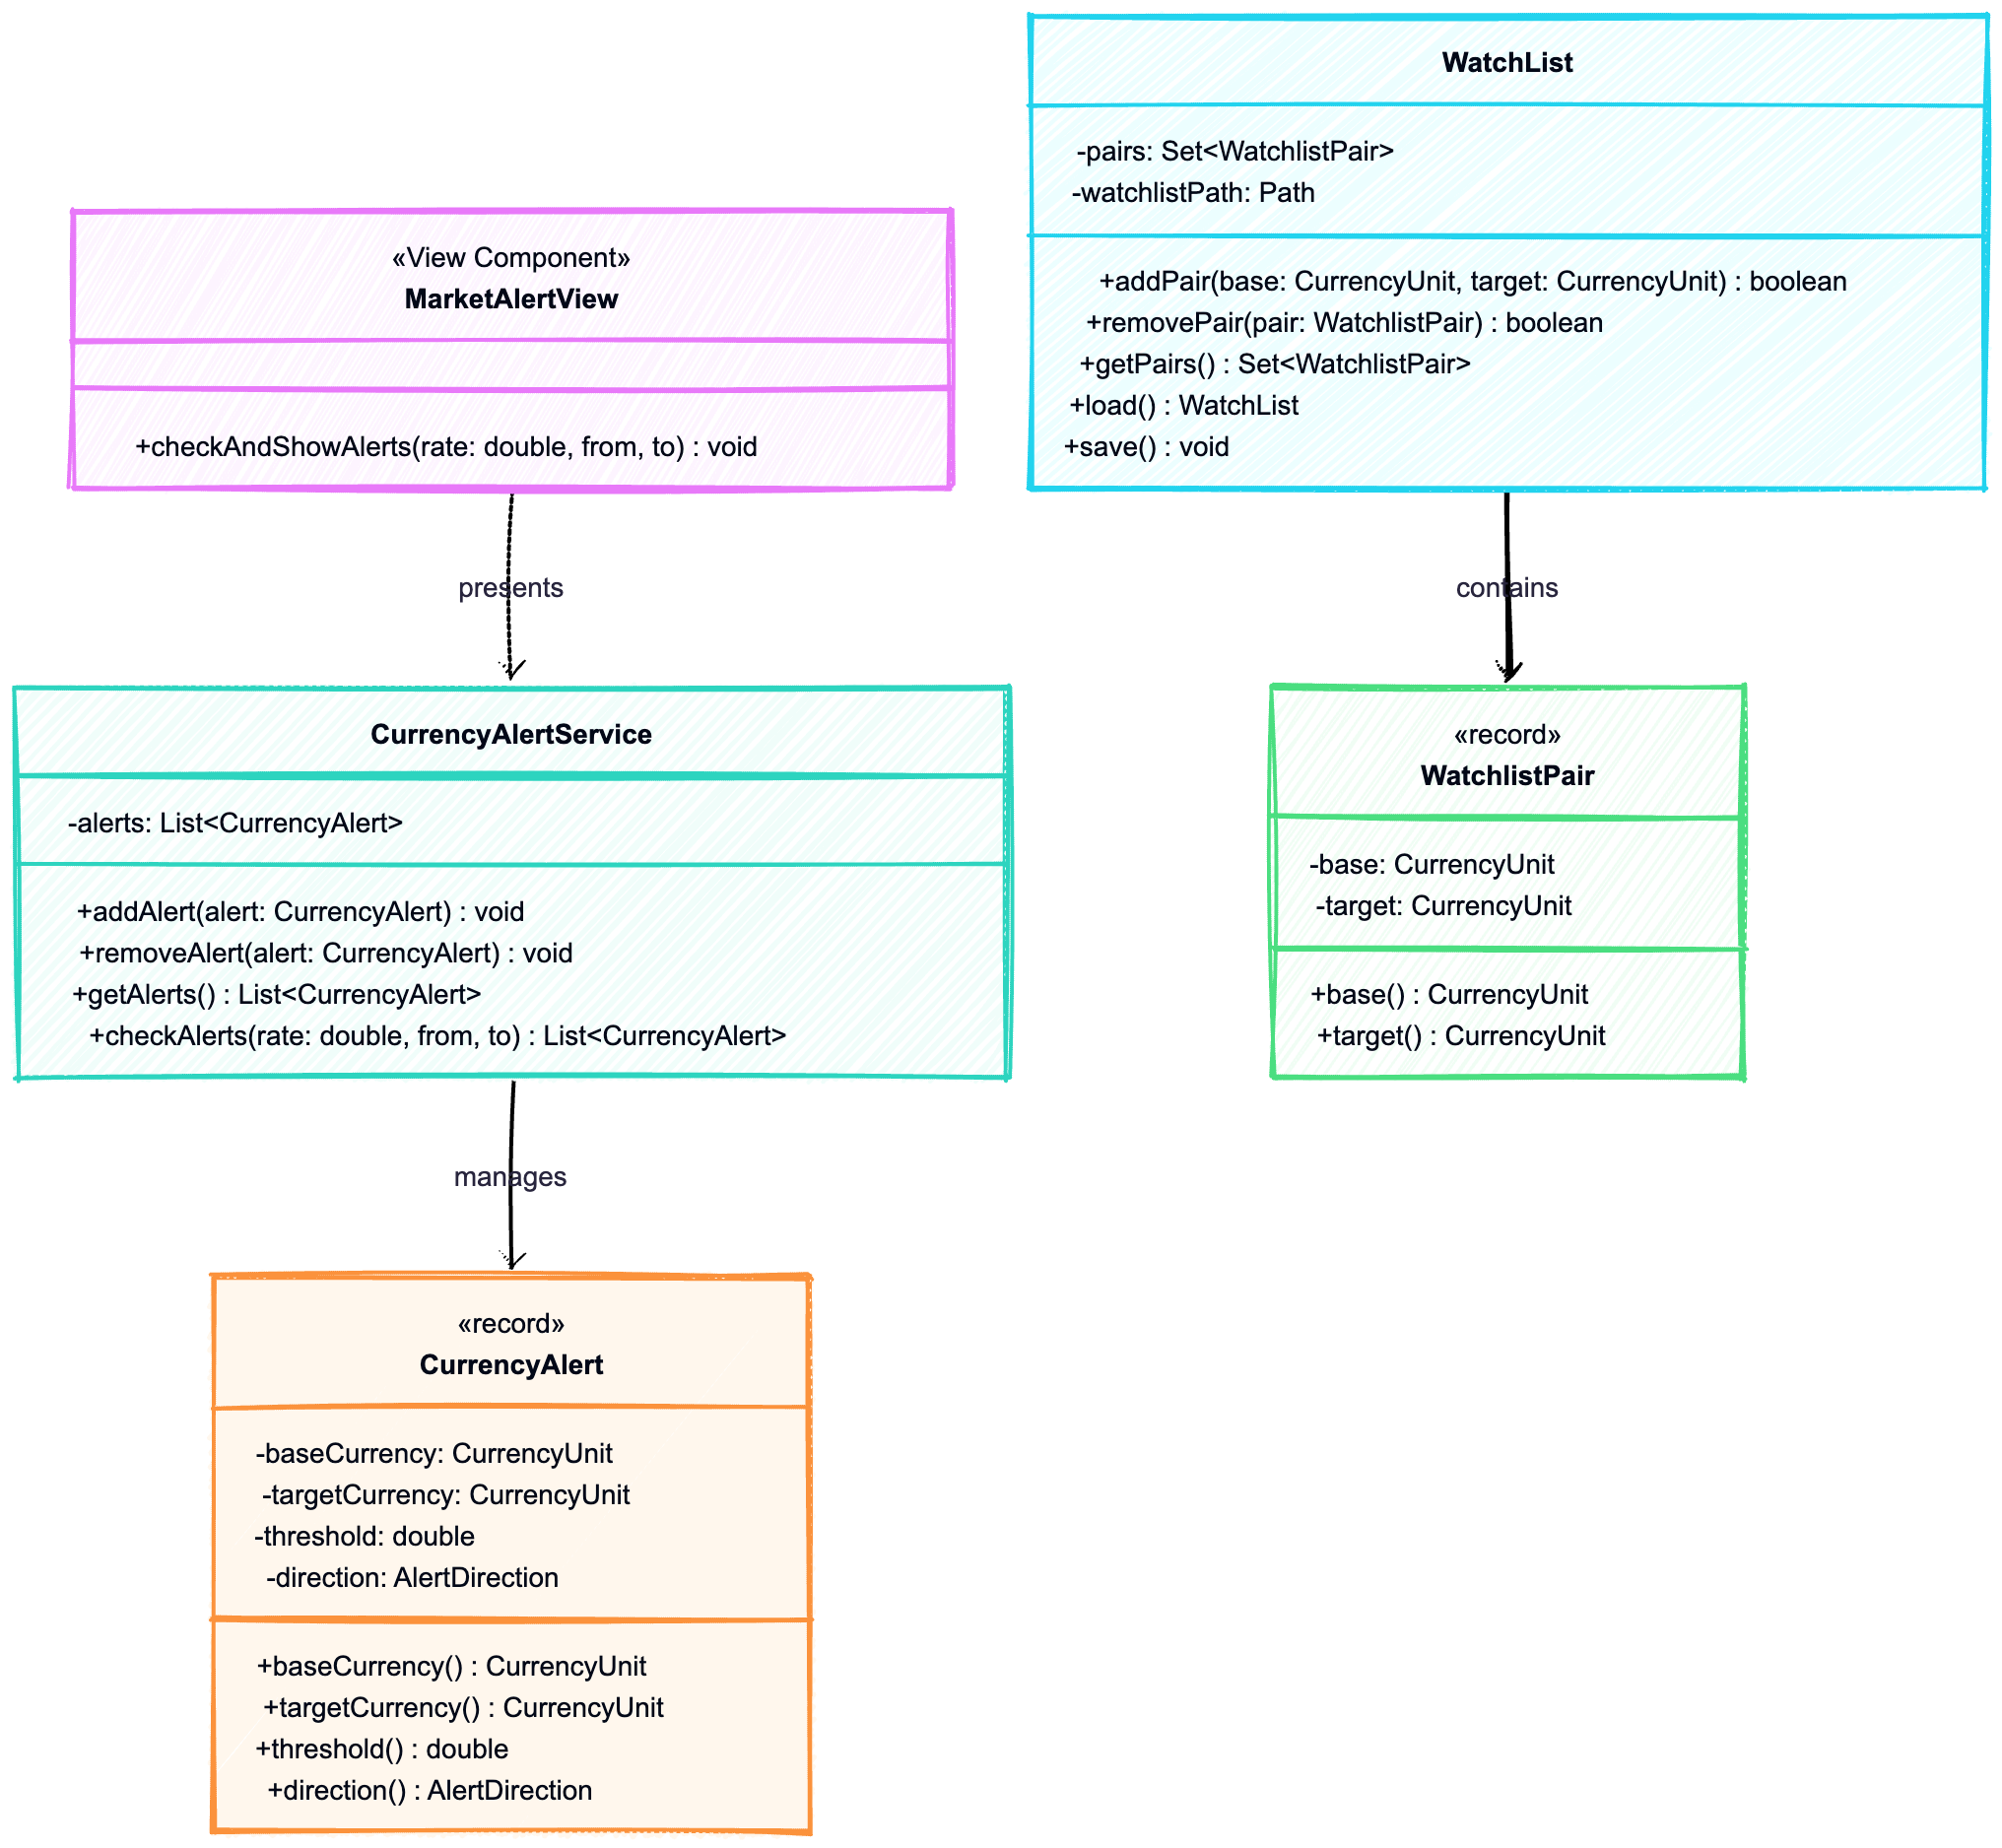
\includegraphics[
        width=0.95\textwidth,
        keepaspectratio
    ]{img/uml-alert-watchlist.png}
    \caption{Diagramma delle classi: monitoraggio delle soglie, emissione delle allerte e gestione persistente della watchlist.}
    \label{fig:alert-watchlist}
\end{figure}

\subsubsection*{4. Pattern utilizzati e reificazione}
\begin{itemize}
    \item \textbf{Observer Pattern:} \texttt{CurrencyAlertService} funge da soggetto di monitoraggio. Quando viene registrato un nuovo tasso di cambio durante una conversione, il servizio valuta le soglie e notifica i componenti della View (\texttt{MarketAlertView}) affinché presentino l'avviso all'utente.
    \item \textbf{Defensive Design:} \texttt{WatchList} restituisce collezioni immutabili (\texttt{Collections.unmodifiableSet}) per proteggere lo stato interno da manipolazioni esterne non autorizzate.
\end{itemize}

% ----------------------------------------------------------------------------
\subsection{Gestione delle Preferenze Utente, Temi Dinamici e Memento dello Stato}

\subsubsection*{1. Descrizione del problema}
L'ergonomia dell'applicazione prevede la completa personalizzazione dello spazio operativo: selezione della valuta di conto globale (con ricalcolo a catena dei totali di portafoglio), commutazione tra tema cromatico chiaro (\emph{Light}) e scuro (\emph{Dark}), regolazione della scala tipografica e persistenza delle dimensioni geometriche della finestra principale. Questo scenario imponeva due requisiti architetturali:
\begin{enumerate}
    \item \textbf{Ripristino dello Stato Pregresso (Undo/Restore):} Possibilità per l'utente di annullare modifiche accidentali in modifica del tema;
    \item \textbf{Propagazione dei Fogli di Stile a Caldo (Hot Theme Swapping):} Aggiornamento istantaneo dell'aspetto visivo di tutte le scene e finestre modali attive senza richiedere il riavvio dell'applicazione e senza distruggere i nodi grafici dello SceneGraph.
\end{enumerate}

\subsubsection*{2. Soluzione proposta e alternative}
\begin{itemize}
    \item \textbf{Alternativa scartata A (Variabili globali statiche sparse):} Mantenere impostazioni come variabili statiche distribuite nei controller genera accoppiamento occulto, impedisce il testing parallelo ed espone lo stato ad alterazioni concorrenti non controllate.
    \item \textbf{Alternativa scartata B (Riavvio forzato dell'applicazione):} Costringere l'utente a riavviare l'applicazione per applicare un tema o una valuta base comporta una grave degradazione dell'usabilità e la potenziale perdita di dati non salvati nelle form aperte.
    \item \textbf{Soluzione adottata:}
    \begin{itemize}
        \item \emph{Reificazione del Memento Pattern:} La classe \texttt{Settings} opera come \emph{Originator}, incapsulando lo stato corrente e generando istantanee immutabili \texttt{SettingsSnapshot} (\emph{Memento}) complete di timestamp, valuta e tema; il manager persistente \texttt{SettingsManager} funge da \emph{Caretaker}, archiviando lo storico delle istantanee e fornendo il metodo \texttt{restoreSnapshot()} per ripristinare uno stato passato in modo atomico;
        \item \emph{Registro centralizzato di stile nella View (\texttt{ThemeManager}):} Collocato nel package della vista (\texttt{it.unibo.unibodget.view.settings}), il manager centralizza la gestione dei fogli di stile. Il metodo \texttt{ThemeManager.applyThemeToScene(Scene)} manipola direttamente la collezione \texttt{scene.getStylesheets()}, iniettando a runtime le classi CSS radice (\texttt{.theme-dark} vs \texttt{.theme-light}) con ricalcolo immediato del rendering da parte del motore grafico JavaFX.
    \end{itemize}
\end{itemize}

\subsubsection*{3. Schema UML e Interazioni}
La struttura del sistema di gestione delle configurazioni, la reificazione del pattern Memento e la propagazione dello stile tramite Observer sono presentate nel seguente diagramma:

\begin{figure}[H]
\centering
\resizebox{0.95\textwidth}{!}{
\begin{tikzpicture}[
    umlclass/.style={
        draw=blue!65!black,
        fill=white,
        rectangle split,
        rectangle split parts=3,
        rectangle split part fill={blue!6, white, white},
        rounded corners=2pt,
        font=\scriptsize,
        align=left
    },
    uses/.style={thick, -{Stealth[scale=0.8]}},
    duses/.style={thick, dashed, -{Stealth[scale=0.8]}}
]
\node[umlclass] (manager) at (0, 6.2) {
    \hfil \textbf{SettingsManager (Caretaker)} \hfil
    \nodepart{second}
    - settings : Settings \\
    - history : List~SettingsSnapshot~
    \nodepart{third}
    + getSettings() : Settings \\
    + saveSettings(settings : Settings) : void \\
    + getHistory() : List~SettingsSnapshot~ \\
    + restoreSnapshot(snapshot : SettingsSnapshot) : void
};

\node[umlclass] (settings) at (-4.8, 1.8) {
    \hfil \textbf{Settings (Originator)} \hfil
    \nodepart{second}
    - theme : Theme \\
    - baseCurrency : CurrencyUnit \\
    - windowPreferences : WindowPreferences
    \nodepart{third}
    + createSnapshot() : SettingsSnapshot \\
    + restoreFromSnapshot(snapshot : SettingsSnapshot) : void \\
    + getTheme() : Theme \\
    + setTheme(Theme) : void
};

\node[umlclass] (snapshot) at (4.8, 1.8) {
    \hfil \textbf{\guillemotleft record\guillemotright} \hfil \\ \hfil \textbf{SettingsSnapshot (Memento)} \hfil
    \nodepart{second}
    - timestamp : Instant \\
    - theme : Theme \\
    - baseCurrency : CurrencyUnit
    \nodepart{third}
    + timestamp() : Instant \\
    + theme() : Theme \\
    + baseCurrency() : CurrencyUnit
};

\node[umlclass] (themeMgr) at (-4.8, -3.2) {
    \hfil \textbf{\guillemotleft Observer / CSS Registry\guillemotright} \hfil \\ \hfil \textbf{ThemeManager} \hfil
    \nodepart{second}
    - currentTheme : Theme \\
    - registeredScenes : List~Scene~
    \nodepart{third}
    + applyThemeToScene(scene : Scene) : void \\
    + registerScene(scene : Scene) : void \\
    + getCurrentTheme() : Theme \\
    + setTheme(theme : Theme) : void
};

\draw[uses] (manager.south) -- ++(-2.2, -0.6) -| node[near end, left, font=\scriptsize] {persists} (settings.north);
\draw[uses] (manager.south) -- ++(2.2, -0.6) -| node[near end, right, font=\scriptsize] {stores history} (snapshot.north);
\draw[uses] (settings) -- node[above, font=\scriptsize] {creates / restores} (snapshot);
\draw[duses] (settings.south) -- node[right, font=\scriptsize] {notifies} (themeMgr.north);

\end{tikzpicture}
}
\caption{Diagramma delle classi: reificazione del Memento Pattern per le impostazioni e Observer per l'iniezione dinamica del tema.}
\label{fig:memento-theme}
\end{figure}

\subsubsection*{4. Pattern utilizzati e reificazione}
\begin{itemize}
    \item \textbf{Memento Pattern:} \texttt{Settings} riveste il ruolo di \emph{Originator}; \texttt{SettingsSnapshot} costituisce il \emph{Memento}; \texttt{SettingsManager} e \texttt{SettingsController} operano come \emph{Caretaker}, gestendo la lista di snapshot senza violarne l'incapsulamento.
    \item \textbf{Observer Pattern:} \texttt{ThemeManager} notifica i listener registrati a ogni modifica di stile, sincronizzando istantaneamente la palette di tutti i componenti aperti.
\end{itemize}

% ----------------------------------------------------------------------------
\subsection{Composizione, Accessibilità e Ottimizzazione della View}

\subsubsection*{1. Descrizione del problema}
La sezione di conversione non è un semplice modulo elementare, ma integra quattro widget visivi interattivi e complessi:
\begin{enumerate}
    \item \texttt{ConverterWidgetFX}: calcolatore di cambio diretto tra valute con controlli di validazione e innesco delle allerte.
    \item \texttt{BankConverterWidgetFX}: simulatore dei tassi bancari reali con spread e commissioni accessorie.
    \item \texttt{CurrencyHistoryChartView}: grafico a linee che traccia l'andamento del cambio in un intervallo di date.
    \item \texttt{WatchlistWidgetFX}: pannello di monitoraggio rapido delle coppie preferite.
\end{enumerate}
Oltre alla necessità di aggregare questi componenti mantenendoli totalmente disaccoppiati dalla shell principale, si sono presentate due sfide ergonomiche e visive rilevanti:
\begin{itemize}
    \item \textbf{Troncamento del selettore di direzione (\emph{Above/Below}):} Nel pannello allerte del convertitore, il testo dell'etichetta veniva visualizzato tronco (es. "Abo...") a causa di un conflitto tra selettori CSS globali (\texttt{.theme-dark .combo-box}) e locali con padding eccessivo, unitamente a vincoli di layout troppo rigidi.
    \item \textbf{Adattamento dinamico del layout del pannello:} Quando la finestra viene ridimensionata e lo spazio orizzontale disponibile si riduce, l'interfaccia riorganizza automaticamente i componenti, disponendoli su più righe anziché mantenerli affiancati. In particolare, alcuni elementi vengono spostati nella parte inferiore del pannello per garantire una visualizzazione più ordinata e leggibile. Per gestire il contenuto che eccede lo spazio verticale disponibile, viene inoltre introdotta una barra di scorrimento sul lato destro, che consente di accedere a tutti gli elementi senza compromettere il layout.
\end{itemize}

\subsubsection*{2. Soluzione proposta e alternative}
\begin{itemize}
    \item \textbf{Alternativa scartata (Controller unico con codice FXML monolitico):} Riunire tutti i controlli in un unico mega-controller avrebbe generato un'anti-architettura difficilmente manutenibile e incline a violazioni di SpotBugs e Checkstyle.
    \item \textbf{Soluzione architetturale adottata:} Scomposizione in singoli widget autonomi dotati di visibilità package-private, orchestrati dalla classe \texttt{CurrencyConverterViewFX} ed esposti alla shell applicativa mediante \texttt{CurrencyConverterModule}.
    \item \textbf{Risoluzione dei conflitti di stile e specificità CSS:}
    \begin{itemize}
        \item Per il selettore \texttt{directionBox}, è stata innalzata la specificità nel foglio di stile \texttt{theme.css} introducendo selettori contestualizzati (\texttt{.theme-dark .direction-box}, \texttt{.direction-box .cell}, \texttt{.direction-box .arrow-button}) con padding azzerato o controllato, stabilendo una larghezza minima di sicurezza (\texttt{125px}) e preferita (\texttt{130px}) e imponendo \texttt{HBox.setHgrow(directionBox, Priority.NEVER)} per prevenire compressioni indebite.
        \item \textbf{Adattamento dinamico del layout del pannello:} Quando la finestra viene ridimensionata e lo spazio orizzontale disponibile si riduce, l'interfaccia riorganizza automaticamente i componenti, disponendoli su più righe anziché mantenerli affiancati. In particolare, alcuni elementi vengono spostati nella parte inferiore del pannello per garantire una visualizzazione più ordinata e leggibile. Per gestire il contenuto che eccede lo spazio verticale disponibile, viene inoltre introdotta una barra di scorrimento sul lato destro, che consente di accedere a tutti gli elementi senza compromettere il layout.
    \end{itemize}
\end{itemize}

\subsubsection*{3. Schema UML e Interazioni}
L'architettura composita della vista del convertitore è strutturata come segue:

\begin{figure}[H]
\centering
\resizebox{0.95\textwidth}{!}{
\begin{tikzpicture}[
    umlclass/.style={
        draw=blue!65!black,
        fill=white,
        rectangle split,
        rectangle split parts=3,
        rectangle split part fill={blue!6, white, white},
        rounded corners=2pt,
        font=\scriptsize,
        align=left
    },
    uses/.style={thick, -{Stealth[scale=0.8]}},
    duses/.style={thick, dashed, -{Stealth[scale=0.8]}}
]
\node[umlclass] (module) at (0, 7.8) {
    \hfil \textbf{CurrencyConverterModule} \hfil
    \nodepart{second}
    - view : CurrencyConverterViewFX \\
    - controller : CurrencyConverterController
    \nodepart{third}
    + getView() : Node \\
    + getController() : CurrencyConverterController
};

\node[umlclass] (facade) at (0, 4.0) {
    \hfil \textbf{\guillemotleft Facade\guillemotright} \hfil \\ \hfil \textbf{CurrencyConverterViewFX} \hfil
    \nodepart{second}
    - converterWidget : ConverterWidgetFX \\
    - bankWidget : BankConverterWidgetFX \\
    - chartWidget : CurrencyHistoryChartView \\
    - watchlistWidget : WatchlistWidgetFX
    \nodepart{third}
    + getView() : Parent
};

\node[umlclass] (conv) at (-5.5, 0.2) {
    \hfil \textbf{ConverterWidgetFX} \hfil
    \nodepart{second}
    - amountField : TextField \\
    - fromBox : ComboBox \\
    - toBox : ComboBox
    \nodepart{third}
    + getView() : Node
};

\node[umlclass] (bank) at (5.5, 0.2) {
    \hfil \textbf{BankConverterWidgetFX} \hfil
    \nodepart{second}
    - bankCombo : ComboBox \\
    - amountField : TextField \\
    - netAmountLabel : Label
    \nodepart{third}
    + getView() : Node
};

\node[umlclass] (chart) at (-5.5, -3.8) {
    \hfil \textbf{CurrencyHistoryChartView} \hfil
    \nodepart{second}
    - chart : LineChart \\
    - fromDatePicker : DatePicker \\
    - toDatePicker : DatePicker
    \nodepart{third}
    + getView() : Node
};

\node[umlclass] (watch) at (5.5, -3.8) {
    \hfil \textbf{WatchlistWidgetFX} \hfil
    \nodepart{second}
    - tableView : TableView \\
    - baseBox : ComboBox
    \nodepart{third}
    + getView() : Node
};

\draw[uses] (module) -- node[right, font=\scriptsize] {orchestrates} (facade);
\draw[uses] (facade.south) -- ++(-2.2, -0.6) -| (conv.north);
\draw[uses] (facade.south) -- ++(2.2, -0.6) -| (bank.north);

% Outer bypass arrows passing cleanly on the outside
\draw[uses] (facade.west) -- ++(-5.5, 0) |- (chart.west);
\draw[uses] (facade.east) -- ++(5.5, 0) |- (watch.east);

\end{tikzpicture}
}
\caption{Diagramma delle classi: scomposizione modulare e composizione dei widget della vista del convertitore.}
\label{fig:view-composition-diagram}
\end{figure}

\subsubsection*{4. Pattern utilizzati e reificazione}
\begin{itemize}
    \item \textbf{Facade Pattern:} \texttt{CurrencyConverterViewFX} funge da \emph{Facade} per l'intero sottosistema grafico del convertitore, nascondendo alla shell principale i dettagli dell'albero JavaFX e offrendo un punto d'ingresso pulito.
    \item \textbf{Module Pattern:} \texttt{CurrencyConverterModule} incapsula il ciclo di vita del modulo, istanziando il rispettivo controller e adottando la \emph{Lazy Initialization} per la costruzione della vista, riducendo l'impronta di memoria e velocizzando il bootstrap dell'app.
\end{itemize}

% ----------------------------------------------------------------------------
\subsection{Risoluzione Resiliente del File System e Autoconsistenza dei Dati (AppDataPathResolver)}

\subsubsection*{1. Descrizione del problema}
Nelle prime versioni dell'applicazione, ciascuna classe responsabile della persistenza sul disco (tra cui \texttt{SettingsManager}, \texttt{ThemeList}, \texttt{InvestmentAccountManager}, \texttt{CashAccountManager}, \texttt{CategoryManager}, \texttt{BankList}, \texttt{Currency} e \texttt{WatchList}) definiva in modo rigido e duplicato il percorso fisico dei file (\texttt{Path.of("data/json/...")}). Tale approccio presentava gravi limiti di progettazione e usabilità:
\begin{enumerate}
    \item \textbf{Violazione del Single Source of Truth:} La moltiplicazione di costanti di percorso cablate impediva qualsiasi riconfigurazione trasparente della cartella dati, richiedendo modifiche ad otto classi distinte in caso di variazione strutturale.
    \item \textbf{Fragilità d'avvio da sottocartelle o ambienti eterogenei:} Se l'applicazione veniva eseguita impostando come working directory una cartella diversa dalla radice del repository (ad esempio lanciando test o task da una sottodirectory o da contesti IDE esterni), l'accesso relativo a \texttt{./data} falliva, provocando il mancato caricamento dei dati utente.
    \item \textbf{Dispersione accidentale dei dati:} In caso di riposizionamento involontario della cartella dati sul computer dell'utente (ad esempio spostamento su Scrivania o Download), l'applicazione non disponeva di alcun meccanismo euristico di rilevamento e procedeva alla generazione forzata di dati vuoti, con potenziale disorientamento per l'utente.
\end{enumerate}

\subsubsection*{2. Soluzione proposta e alternative}
\begin{itemize}
    \item \textbf{Alternativa scartata (Passaggio obbligatorio di parametri da riga di comando):} Richiedere all'utente di specificare sempre un parametro JVM (es. \texttt{-Dunibodget.data.dir=...}) avrebbe peggiorato l'usabilità immediata del software.
    \item \textbf{Alternativa scartata (Scansione globale ricorsiva del disco):} Una ricerca cieca sull'intero albero del file system avrebbe introdotto ritardi inaccettabili in fase di avvio, esponendosi al rischio di blocchi dovuti a permessi di accesso o collegamenti ciclici.
    \item \textbf{Soluzione adottata:} Centralizzazione della risoluzione in una classe dedicata, \texttt{AppDataPathResolver}, fondata su una gerarchia rigorosa a quattro livelli di priorità:
    \begin{enumerate}
        \item \textbf{Passo 1 (Data locale standard):} Se la directory \texttt{./data} esiste nella cartella di lavoro corrente, viene selezionata ed impiegata immediatamente. Questa scelta azzera qualsiasi latenza di scansione (\emph{zero search overhead}) e assicura il 100\% di continuità e stabilità rispetto al comportamento standard.
        \item \textbf{Passo 2 (Ricerca euristica intelligente delimitata):} Qualora la cartella locale non sia presente, il resolver innesca un'indagine controllata e protetta da vincoli stringenti:
        \begin{itemize}
            \item Esamina percorsi adiacenti frequenti (\texttt{../data}, \texttt{../../data}, \texttt{app/data}, \texttt{\textasciitilde/.unibodget/data}).
            \item Scansiona le directory utente canoniche (Desktop, Documents, Downloads e radice superiore) con profondità massima limitata a 3 livelli (\texttt{MAX\_SEARCH\_DEPTH = 3}), fermando l'ispezione al raggiungimento di 500 cartelle visitate e saltando a priori rami nascosti (\texttt{.git}, \texttt{.gradle}) e cartelle di build (\texttt{build}, \texttt{bin}, \texttt{target}, \texttt{node\_modules}, \texttt{Library}).
            \item Sottopone ciascun candidato a \textbf{validazione semantica}: il file \texttt{json/settings/Settings.json} deve esistere, essere leggibile e contenere campi JSON proprietari di UniBodget (\texttt{baseCurrency}, \texttt{theme}), eliminando alla radice il rischio di falsi positivi su cartelle omonime di terze parti.
        \end{itemize}
        \item \textbf{Passo 3 (Parametro esplicito opzionale):} Se la ricerca euristica non rileva cartelle preesistenti, il resolver verifica la presenza della proprietà JVM di sistema \texttt{unibodget.data.dir} o della variabile d'ambiente \texttt{UNIBODGET\_DATA\_DIR}.
        \item \textbf{Passo 4 (Clean fallback con self-healing):} Come garanzia conclusiva di funzionamento, il resolver ricade sul percorso standard \texttt{Path.of("data")}. Qualora i file non esistano, \texttt{ModelFileManager} interviene in modalità di \emph{self-healing}, estraendo automaticamente i template JSON predefiniti inclusi nel classpath applicativo (\texttt{resources/json/}).
    \end{enumerate}
\end{itemize}

\subsubsection*{3. Schema UML e Interazioni}
Il ruolo centrale di \texttt{AppDataPathResolver} come punto di disaccoppiamento e l'interazione con le classi persistenti sono illustrati nel seguente diagramma:

\begin{figure}[H]
\centering
\resizebox{0.95\textwidth}{!}{
\begin{tikzpicture}[
    umlclass/.style={
        draw=blue!65!black,
        fill=white,
        rectangle split,
        rectangle split parts=3,
        rectangle split part fill={blue!6, white, white},
        rounded corners=2pt,
        font=\scriptsize,
        align=left
    },
    uses/.style={thick, -{Stealth[scale=0.8]}},
    duses/.style={thick, dashed, -{Stealth[scale=0.8]}}
]
\node[umlclass] (resolver) at (0, 3.8) {
    \hfil \textbf{\guillemotleft Single Source of Truth\guillemotright} \hfil \\ \hfil \textbf{AppDataPathResolver} \hfil
    \nodepart{second}
    - DATA\_DIR\_NAME : String = "data" \\
    - MAX\_SEARCH\_DEPTH : int = 3 \\
    - MAX\_VISITED\_DIRECTORIES : int = 500 \\
    - cachedDataDir : Path
    \nodepart{third}
    + getDataDir() : Path \\
    + resolve(relativePath : String) : Path \\
    + resolveJson(subpath : String) : Path \\
    + resolveCsv(subpath : String) : Path \\
    + isValidUniBodgetDataDir(candidate : Path) : boolean \\
    + setCustomDataDir(path : Path) : void \\
    + reset() : void
};

\node[umlclass] (fileMgr) at (0, -1.8) {
    \hfil \textbf{\guillemotleft Self-Healing\guillemotright} \hfil \\ \hfil \textbf{ModelFileManager} \hfil
    \nodepart{second}
    \nodepart{third}
    + ensureFileExists(target : Path,\\~~~~resourceTemplate : String) : void
};

\node[umlclass] (sm) at (-7.2, 5.0) {
    \hfil \textbf{SettingsManager} \hfil
    \nodepart{second}
    - settingsFilePath : Path
    \nodepart{third}
    + getSettings() : Settings \\
    + saveSettings(...) : void
};

\node[umlclass] (bl) at (-7.2, 1.8) {
    \hfil \textbf{BankList} \hfil
    \nodepart{second}
    - bankFilePath : Path
    \nodepart{third}
    + getBanks() : List~Bank~
};

\node[umlclass] (tl) at (7.2, 5.0) {
    \hfil \textbf{ThemeList} \hfil
    \nodepart{second}
    - themesFilePath : Path
    \nodepart{third}
    + getThemes() : List~Theme~
};

\node[umlclass] (wl) at (7.2, 1.8) {
    \hfil \textbf{WatchList} \hfil
    \nodepart{second}
    - watchlistPath : Path
    \nodepart{third}
    + load() : WatchList
};

\draw[duses] (resolver.south) -- node[right, font=\scriptsize] {fallback templates} (fileMgr.north);
\draw[duses] (sm.east) -- node[above, font=\scriptsize] {resolveJson} (resolver.west |- sm.east);
\draw[duses] (bl.east) -- node[above, sloped, font=\scriptsize] {resolveJson} (resolver.south west);
\draw[duses] (tl.west) -- node[above, font=\scriptsize] {resolveJson} (resolver.east |- tl.west);
\draw[duses] (wl.west) -- node[above, sloped, font=\scriptsize] {resolveJson} (resolver.south east);

\end{tikzpicture}
}
\caption{Diagramma delle classi: architettura del percorso dati centralizzato e relazioni con i manager di persistenza.}
\label{fig:resolver-diagram}
\end{figure}

\subsubsection*{4. Pattern utilizzati e reificazione}
\begin{itemize}
    \item \textbf{Chain of Responsibility / Strategy Pattern:} La selezione della directory di lavoro incapsula una sequenza di strategie di lookup ordinate per priorità, arrestandosi al verificarsi della prima condizione soddisfacente.
    \item \textbf{Single Source of Truth:} Tutte le 8 classi persistenti sono state disaccoppiate e collegate ad \texttt{AppDataPathResolver.resolveJson(...)} e \texttt{resolveCsv(...)}, garantendo che qualsiasi modifica logistica della cartella dati si propaghi istantaneamente e uniformemente a tutta l'applicazione.
    \item \textbf{Design for Testability:} La classe mette a disposizione i metodi \texttt{setCustomDataDir(Path)} e \texttt{reset()}, consentendo alle suite di test automatizzati di operare su directory temporanee isolate (\texttt{@TempDir}) senza interferire con lo stato persistente reale dell'applicazione.
\end{itemize}

% ----------------------------------------------------------------------------
\subsection{Normalizzazione del Parsing e Validazione dell'Input Monetario (MonetaryInputParser)}

\subsubsection*{1. Descrizione del problema}
Nelle applicazioni gestionali e finanziarie, l'interazione con l'utente sui campi di inserimento numerico (importi di spesa, quote di budget, tassi di cambio, soglie di allerta e commissioni) presenta una forte eterogeneità di convenzioni sintattiche:
\begin{itemize}
    \item La notazione standard internazionale impiega il punto (\texttt{.}) come delimitatore decimale (es. \texttt{1250.50}).
    \item La convenzione italiana ed europea fa uso della virgola (\texttt{,}) come separatore dei decimali (es. \texttt{1250,50}).
    \item L'utente inserisce frequentemente spaziature non intenzionali prima, dopo o all'interno dell'importo (es. copia-incolla con spazi di raggruppamento delle migliaia come \texttt{"1 250,50"} o apostrofi di formattazione bancaria come \texttt{"1'250.50"}).
\end{itemize}
Nel design originario, ciascuna finestra di dialogo e ciascun widget del modulo (\texttt{ConverterWidgetFX}, \texttt{BankConverterWidgetFX}, \texttt{CurrencyHistoryChartView}, unitamente ai dialoghi della dashboard \texttt{NewTransactionDialog} ed \texttt{EditBudgetDialog}) implementava logiche di parsing frammentate e non uniformi: alcune chiamavano direttamente \texttt{new BigDecimal(text)}, che solleva improvvisamente un'eccezione non controllata \texttt{NumberFormatException} in presenza di virgole o caratteri non canonici; altre applicavano sostituzioni parziali (\texttt{.replace(',', '.')}) senza alcuna validazione formale della struttura; altre ricorrevano a \texttt{Double.parseDouble(text)}, esponendosi alle tipiche imperfezioni di arrotondamento binario a virgola mobile.

\subsubsection*{2. Soluzione proposta e alternative}
\begin{itemize}
    \item \textbf{Alternativa scartata (Gestione isolata con blocchi try-catch in ciascun controller):} Catturare le eccezioni localmente nelle singole classi di vista avrebbe moltiplicato il codice duplicato e lasciato inalterata la fragilità sintattica delle form.
    \item \textbf{Alternativa scartata (Blocco preventivo con regex restrittive nei campi di testo):} Impedire a priori l'inserimento della virgola tramite listener sui \texttt{TextField} avrebbe peggiorato l'usabilità per gli utenti con tastierino numerico o localizzazione italiana.
    \item \textbf{Soluzione adottata:} Progettazione della classe di utilità dedicata \texttt{MonetaryInputParser} all'interno del package \texttt{model.currency}, concepita come \emph{Single Source of Truth} per l'analisi e la validazione degli input monetari dell'intera applicazione:
    \begin{enumerate}
        \item \textbf{Sanitizzazione robusta (\texttt{sanitize}):} Rimuove spazi vuoti iniziali e finali, strip degli spazi di raggruppamento interni, rimozione di apostrofi ed eventuale normalizzazione della virgola nel punto decimale standard.
        \item \textbf{Parsing non bloccante con \texttt{Optional\textless BigDecimal\textgreater} (\texttt{parse}):} Invece di propagare eccezioni a runtime, il metodo restituisce un \texttt{Optional} vuoto in caso di input non parsabile, nullo o non conforme alla grammatica numerica rigorosa (\texttt{\^{}-?\textbackslash\textbackslash{}d+(\textbackslash\textbackslash{}.\textbackslash\textbackslash{}d+)?\$}), favorendo una programmazione funzionale ed elegante nei chiamanti (\texttt{.orElse(null)} o \texttt{.ifPresent()}).
        \item \textbf{Validazioni di dominio con vincoli algebrici:} Fornisce metodi specializzati ad alto livello:
        \begin{itemize}
            \item \texttt{parsePositive(String)}: accetta esclusivamente importi strettamente positivi ($> 0$), ideale per somme da convertire o transazioni;
            \item \texttt{parseNonNegative(String)}: ammette anche il valore zero ($\ge 0$), indispensabile per commissioni bancarie o spread facoltativi;
            \item \texttt{parsePositiveWithMaxScale(String, int)}: valida e limita il numero massimo di cifre decimali ammesse in relazione alla granularità della valuta (es. 2 decimali per FIAT, scale maggiori per Crypto).
        \end{itemize}
        \item \textbf{Adapter per primitive numeriche (\texttt{parseDouble}, \texttt{parsePositiveDouble}, \texttt{parseNonNegativeDouble}):} Offre un'interfaccia coerente anche per i componenti che richiedono coordinate numeriche per grafici o soglie temporanee, garantendo la protezione da \texttt{NaN} e infiniti.
    \end{enumerate}
\end{itemize}

\subsubsection*{3. Schema UML e Interazioni}
L'architettura del parser monetario centralizzato e i componenti di vista che ne fanno uso sono riassunti nel diagramma delle classi seguente:

\begin{figure}[H]
\centering
\resizebox{0.95\textwidth}{!}{
\begin{tikzpicture}[
    umlclass/.style={
        draw=blue!65!black,
        fill=white,
        rectangle split,
        rectangle split parts=3,
        rectangle split part fill={blue!6, white, white},
        rounded corners=2pt,
        font=\scriptsize,
        align=left
    },
    duses/.style={thick, dashed, -{Stealth[scale=0.8]}}
]
\node[umlclass] (parser) at (0, 5.2) {
    \hfil \textbf{\guillemotleft Single Source of Truth\guillemotright} \hfil \\ \hfil \textbf{MonetaryInputParser} \hfil
    \nodepart{second}
    - DECIMAL\_DELIMITER\_PATTERN : Pattern \\
    - STRICT\_NUMERIC\_PATTERN : Pattern
    \nodepart{third}
    + sanitize(input : String) : String \\
    + parse(input : String) : Optional~BigDecimal~ \\
    + parsePositive(input : String) : Optional~BigDecimal~ \\
    + parseNonNegative(input : String) : Optional~BigDecimal~ \\
    + parsePositiveWithMaxScale(input : String, maxScale : int) : Optional~BigDecimal~ \\
    + parseDouble(input : String) : OptionalDouble \\
    + parsePositiveDouble(input : String) : OptionalDouble \\
    + parseNonNegativeDouble(input : String) : OptionalDouble
};

\node[umlclass] (conv) at (-5.5, 1.2) {
    \hfil \textbf{ConverterWidgetFX} \hfil
    \nodepart{second}
    \nodepart{third}
    - parseDecimal(text) : BigDecimal
};

\node[umlclass] (bank) at (5.5, 1.2) {
    \hfil \textbf{BankConverterWidgetFX} \hfil
    \nodepart{second}
    \nodepart{third}
    - parsePositiveAmount(text) \\
    - parseFee(text)
};

\node[umlclass] (chart) at (-5.5, -2.2) {
    \hfil \textbf{CurrencyHistoryChartView} \hfil
    \nodepart{second}
    \nodepart{third}
    - parseThreshold(text) : OptionalDouble
};

\node[umlclass] (dialog) at (5.5, -2.2) {
    \hfil \textbf{NewTransactionDialog} \hfil
    \nodepart{second}
    \nodepart{third}
    - parseAmount(text) : BigDecimal
};

\draw[duses] (conv.north) -- node[left, font=\scriptsize] {parse} (parser.south -| conv.north);
\draw[duses] (bank.north) -- node[right, font=\scriptsize] {parsePositive} (parser.south -| bank.north);

% Outer bypass arrows for chart and dialog passing cleanly on the outside
\draw[duses] (chart.west) -- ++(-1.8, 0) |- node[near start, left, font=\scriptsize] {parseDouble} (parser.west);
\draw[duses] (dialog.east) -- ++(1.8, 0) |- node[near start, right, font=\scriptsize] {parse} (parser.east);

\end{tikzpicture}
}
\caption{Diagramma delle classi: architettura di validazione e parsing dell'input monetario e relative interazioni con le viste.}
\label{fig:monetary-parser-diagram}
\end{figure}

\subsubsection*{4. Pattern utilizzati e reificazione}
\begin{itemize}
    \item \textbf{Utility Class Pattern:} Costruttore privato difensivo che impedisce l'istanziazione anche via reflection, con metodi statici puri, deterministici e privi di effetti collaterali (\emph{side-effect free}).
    \item \textbf{Optional Pattern \& Eliminazione delle Eccezioni come Flusso di Controllo:} Sostituzione dell'anti-pattern del controllo di flusso basato su eccezioni (\emph{Exception-as-Control-Flow}) con costrutti funzionali espliciti e type-safe.
    \item \textbf{DRY (Don't Repeat Yourself):} Tutte le viste dell'applicazione (convertitore ordinario, convertitore bancario, grafico storico, dialoghi di transazione e di budget) sono state uniformate facendole convergere sull'uso esclusivo di \texttt{MonetaryInputParser}.
\end{itemize}

% ============================================================================
% CAPITOLO 3: SVILUPPO
% ============================================================================
\section{Design Dettagliato (Favour Emuwahen)}

In questa sezione vengono documentate le decisioni architetturali, i pattern di progettazione e le motivazioni tecniche adottate nello sviluppo del sottosistema di mia competenza: la Dashboard interattiva, la contabilità dei Portafogli di Cassa (\emph{Cash Wallets}), la costruzione e validazione delle Transazioni Contanti (\emph{Cash Transactions}), l'analisi comparativa dei Trend Mensili (\emph{Monthly Insights}), il monitoraggio dinamico delle soglie di Budget e il Filtraggio declarativo dello storico movimenti.

\subsection{Coordinamento e Disaccoppiamento della Dashboard (Facade e Passive View)}
\subsubsection*{1. Descrizione del problema}
La Dashboard rappresenta il centro operativo dell'applicazione: deve aggregare ed esporre simultaneamente una pluralità di informazioni eterogenee:
\begin{itemize}
    \item Saldo totale e controvalore convertito nella valuta di riferimento globale;
    \item Ripartizione percentuale e scomposizione delle uscite per categoria;
    \item Stato di avanzamento del budget mensile con percentuale di consumo;
    \item Posizione debitoria/creditoria netta verso amici (\emph{Friend Loans});
    \item Indicatori di tendenza mese su mese (\emph{Monthly Insights});
    \item Cronologia dei movimenti recenti con filtri dinamici di ricerca.
\end{itemize}
Consentire al controller o alla vista di interrogare direttamente i singoli servizi di dominio (gestione conti, categorie, calcolo budget, prestiti, statistiche) avrebbe introdotto un accoppiamento elevatissimo (\emph{tight coupling}), violando la Legge di Demetra e rendendo la View dipendente dai dettagli interni del Model. Inoltre, esporre entità mutabili del dominio alla GUI avrebbe compromesso l'integrità contabile.

\subsubsection*{2. Soluzione proposta e alternative}
\begin{itemize}
    \item \textbf{Alternativa scartata (Controller multi-servizio accoppiato):} Far dialogare il controller direttamente con ciascun servizio avrebbe portato alla creazione di una \emph{God Class} con decine di dipendenze dirette, rendendo complessa la manutenzione e impossibili i test in isolamento.
    \item \textbf{Alternativa scartata (Passaggio di entità di dominio alla View):} Far consumare direttamente \texttt{CashAccount} e \texttt{Category} ai componenti JavaFX espone la rappresentazione interna a manipolazioni esterne non controllate (\emph{representation exposure}).
    \item \textbf{Soluzione adottata:} Introduzione del pattern Facade tramite l'interfaccia \texttt{DashboardFacade} e la classe \texttt{DefaultDashboardFacade}. Il controller invoca un unico metodo ad alto livello (\texttt{loadDashboard()}), che orchestra i sotto-servizi e restituisce un oggetto istantanea immutabile: \texttt{DashboardSnapshot}. Il controller trasforma quindi tale snapshot in una gerarchia di record immutabili di presentazione (\texttt{DashboardViewState}), consegnati alla vista passiva (\texttt{DefaultDashboardView}) per il solo rendering grafico.
\end{itemize}

\subsubsection*{3. Schema UML e Interazioni}
\begin{figure}[H]
\centering
% \includegraphics[width=\textwidth]{img/uml-pattern-dashboard-facade.pdf}
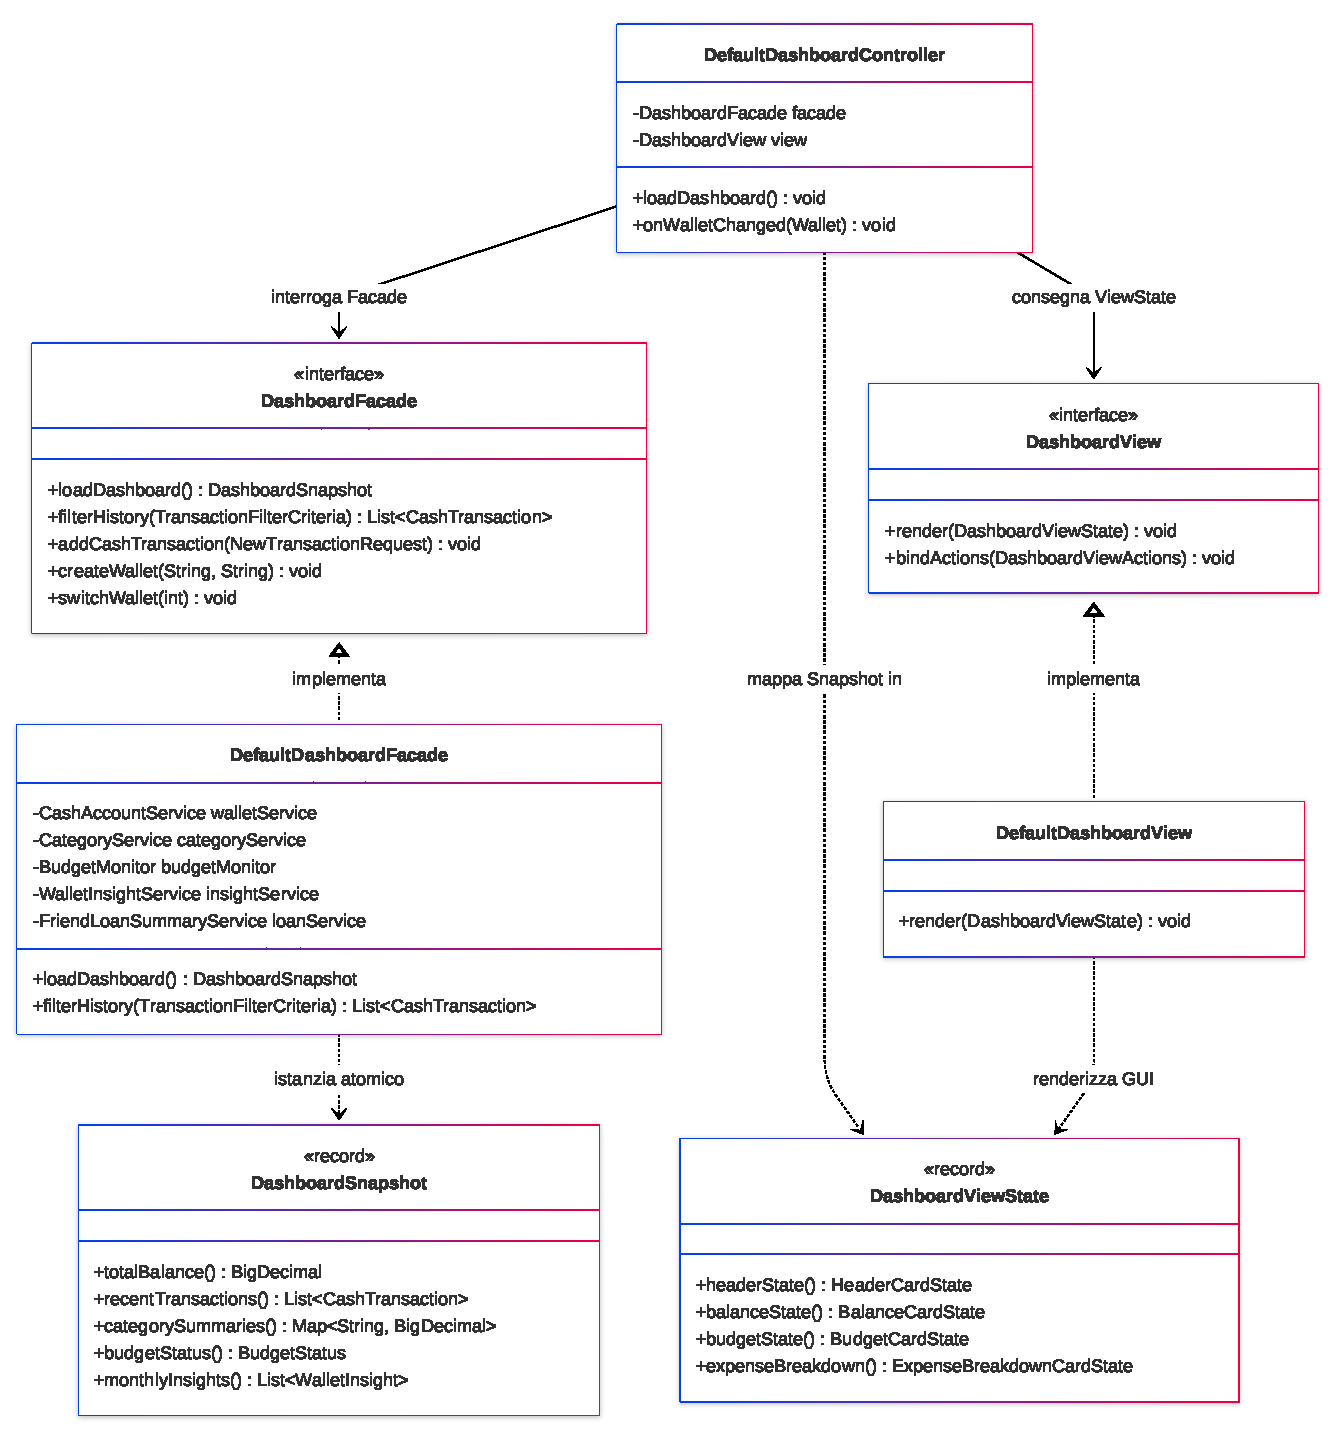
\includegraphics[width=\textwidth]{img/uml-pattern-dashboard-facade.png}
\caption{Reificazione del Facade Pattern e della Passive View per il sottosistema Dashboard.}
\label{fig:dashboard-facade}
\end{figure}

\subsubsection*{4. Pattern utilizzati e reificazione}
\begin{itemize}
    \item \textbf{Facade Pattern:} \texttt{DefaultDashboardFacade} agisce come facciata unificata, incapsulando \texttt{CashAccountService}, \texttt{CategoryService}, \texttt{BudgetMonitor}, \texttt{FriendLoanSummaryService} e \texttt{WalletInsightService}.
    \item \textbf{Value Object / Snapshot Pattern:} \texttt{DashboardSnapshot} raccoglie i dati aggregati del modello all'istante di campionamento, garantendo consistenza atomica.
    \item \textbf{Passive View (MVC):} \texttt{DefaultDashboardView} non accede mai al modello; riceve lo stato \texttt{DashboardViewState} dal controller e notifica le interazioni utente tramite l'interfaccia \texttt{DashboardViewActions}.
    \item \textbf{Observer Pattern:} \texttt{DefaultDashboardController} implementa \texttt{WalletObserver}; quando il servizio portafogli notifica un cambiamento, il controller interroga la facciata e aggiorna reattivamente la vista.
\end{itemize}

\subsection{Costruzione Fluente e Validazione delle Transazioni (Builder e Factory Pattern)}
\subsubsection*{1. Descrizione del problema}
Nel contesto della contabilità di cassa, una transazione monetaria (\texttt{CashTransaction}) presenta una marcata eterogeneità di parametri:
\begin{itemize}
    \item Attributi obbligatori: identificativo univoco (\texttt{UUID}), asset monetario con importo e valuta (\texttt{Asset}), categoria contabile (\texttt{Category}), data di registrazione (\texttt{LocalDate}) e causale;
    \item Attributi contestuali/opzionali: note aggiuntive descrittive, nominativo dell'amico (\texttt{friendName}) e identificativo del prestito correlato (\texttt{friendLoanId}) nel caso di prestiti fiduciari.
\end{itemize}
L'approccio tradizionale basato su costruttori sovraccaricati (\emph{telescoping constructors}) generava confusione e rischio di inversione di argomenti del medesimo tipo (stringhe). D'altro canto, consentire l'uso di setter avrebbe reso l'oggetto mutabile, violando l'integrità contabile. Era inoltre necessario automatizzare la corretta assegnazione del segno algebrico degli importi (es. importi negativi per spese e prestiti erogati, positivi per entrate e restituzioni).

\subsubsection*{2. Soluzione proposta e alternative}
\begin{itemize}
    \item \textbf{Alternativa scartata (Costruttori multipli telescopici):} Impraticabile con l'aumentare dei campi; obbliga a passare parametri null per i valori facoltativi.
    \item \textbf{Alternativa scartata (JavaBeans mutabili):} Scartata categoricamente; in un'applicazione contabile, permettere la modifica di data, importo o categoria post-costruzione espone a corruzioni dello storico.
    \item \textbf{Soluzione adottata:} Implementazione del pattern Builder come classe interna statica fluente (\texttt{CashTransaction.Builder}), coadiuvata dalla classe specializzata Factory (\texttt{CashTransactionFactory}). Il builder valida rigorosamente le invarianti nel metodo terminale \texttt{build()} (es. vincolo di presenza obbligatoria di \texttt{friendName} se la transazione rappresenta un prestito), garantendo che nessuna transazione possa esistere in uno stato incoerente.
\end{itemize}

\subsubsection*{3. Schema UML e Interazioni}
\begin{figure}[H]
\centering
% \includegraphics[width=0.85\textwidth]{img/uml-pattern-cashtransaction.pdf}
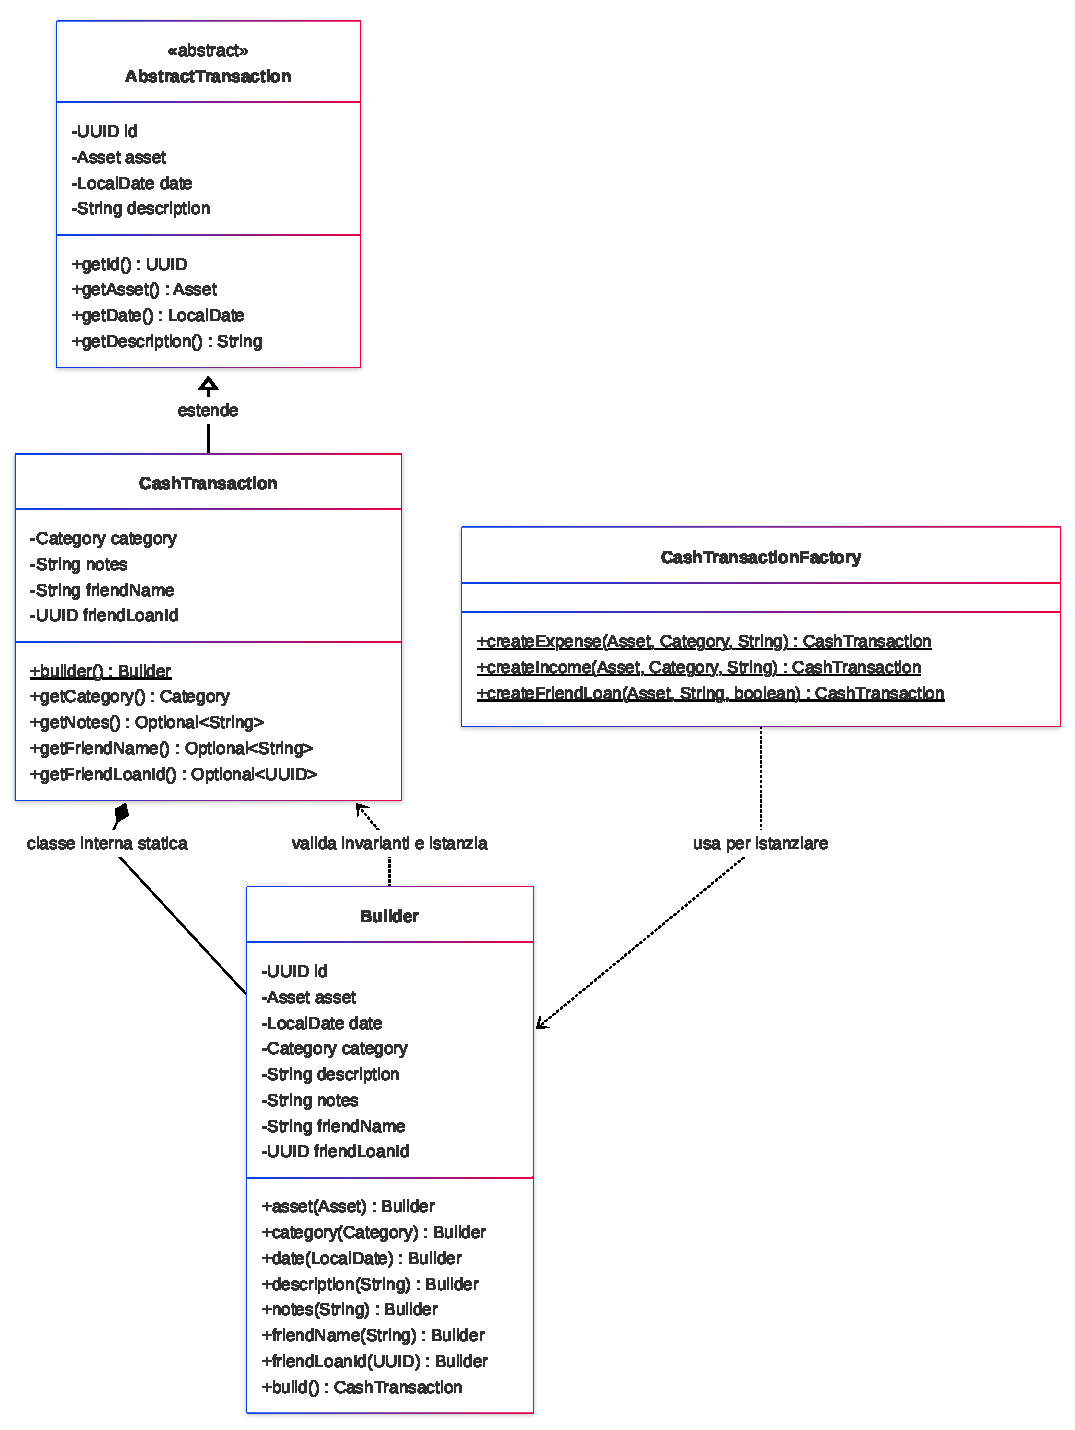
\includegraphics[width=0.85\textwidth]{img/uml-pattern-cashtransaction.png}
\caption{Reificazione dei pattern Builder e Factory per la creazione sicura di CashTransaction.}
\label{fig:transaction-builder}
\end{figure}

\subsubsection*{4. Pattern utilizzati e reificazione}
\begin{itemize}
    \item \textbf{Builder Pattern:} \texttt{CashTransaction.Builder} consente la composizione fluente passo-passo dei parametri, validando le invarianti di business prima di restituire l'oggetto immutabile.
    \item \textbf{Factory Pattern:} \texttt{CashTransactionFactory} incapsula la costruzione dei casi d'uso canonici (\texttt{createExpense}, \texttt{createIncome}, \texttt{createFriendLoan}), gestendo in automatico la polarità degli importi (\texttt{Asset.amount().negate()}) e preservando il principio di singola responsabilità (SRP).
\end{itemize}

\subsection{Monitoraggio Dinamico e Strategie di Allerta del Budget (Strategy Pattern)}
\subsubsection*{1. Descrizione del problema}
Il controllo delle spese rispetto al budget mensile richiede di valutare la spesa cumulativa corrente rispetto al tetto limite prefissato dall'utente e a una soglia percentuale di avviso (es. 80\%). In base al consumo calcolato, il sistema deve emettere un responso qualitativo differenziato (\texttt{SAFE}, \texttt{WARNING}, \texttt{CRITICAL}), corredato da messaggi contestuali e badge cromatici di allerta nella dashboard. La logica di valutazione doveva essere totalmente estendibile, consentendo l'introduzione futura di nuovi criteri di allarme (es. proiezioni di spesa predittiva a metà mese o budget per singola categoria) senza dover modificare il monitor centrale.

\subsubsection*{2. Soluzione proposta e alternative}
\begin{itemize}
    \item \textbf{Alternativa scartata (Istruzioni condizionali annidate nel monitor):} L'uso di ramificazioni if-else o switch cablate all'interno di \texttt{DefaultBudgetMonitor} avrebbe violato il principio Open/Closed (OCP).
    \item \textbf{Soluzione adottata:} Adozione dello Strategy Pattern. L'interfaccia \texttt{BudgetAlertStrategy} definisce il contratto formale per la valutazione algoritmica della spesa. Il monitor (\texttt{DefaultBudgetMonitor}) delega la valutazione alla strategia appropriata, ottenendo come risultato il record immutabile \texttt{BudgetStatus}.
\end{itemize}

\subsubsection*{3. Schema UML e Interazioni}
\begin{figure}[H]
\centering
% \includegraphics[width=\textwidth]{img/uml-pattern-budget-strategy.pdf}
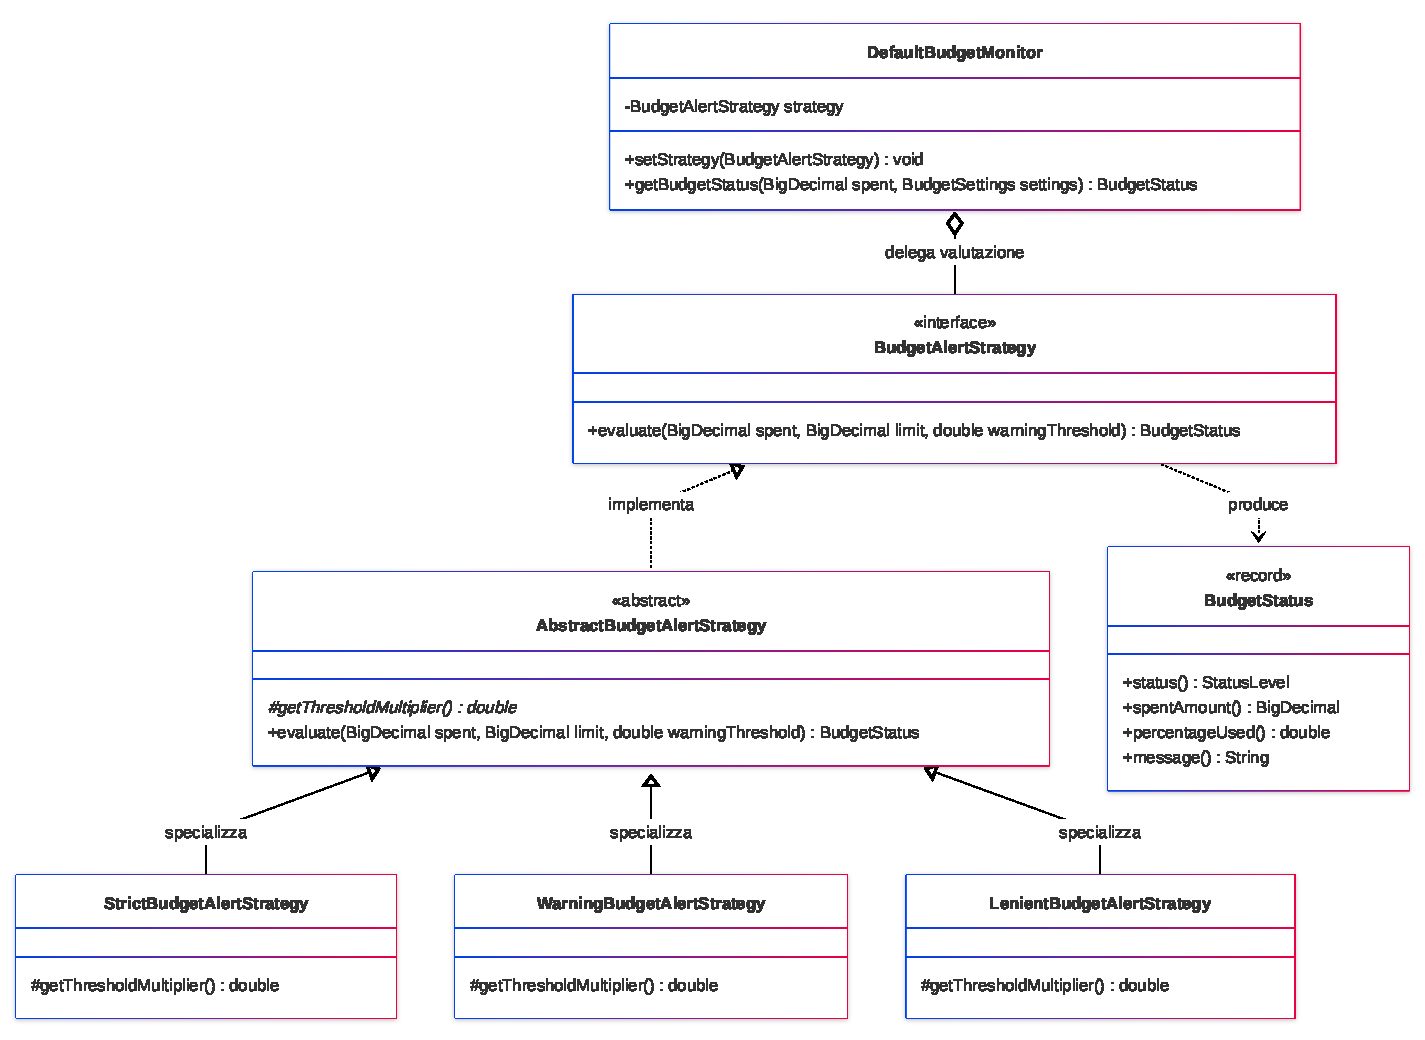
\includegraphics[width=\textwidth]{img/uml-pattern-budget-strategy.png}
\caption{Reificazione dello Strategy Pattern per la valutazione delle soglie di allarme del Budget.}
\label{fig:budget-strategy}
\end{figure}

\subsubsection*{4. Pattern utilizzati e reificazione}
\begin{itemize}
    \item \textbf{Strategy Pattern:} \texttt{BudgetAlertStrategy} costituisce la Strategy astratta; \texttt{SafeBudgetStrategy}, \texttt{WarningBudgetStrategy} e \texttt{CriticalBudgetStrategy} rappresentano le Concrete Strategies. Il client (\texttt{DefaultBudgetMonitor}) agisce da Context, mantenendo completa indipendenza dalle specifiche condizioni di soglia.
    \item \textbf{Open/Closed Principle (OCP):} È possibile introdurre nuove strategie di allerta creando nuove classi che implementano l'interfaccia, senza alterare il codice esistente del monitor.
\end{itemize}

\subsection{Algoritmo di Analisi Comparativa Mensile (Template Method Pattern)}
\subsubsection*{1. Descrizione del problema}
La dashboard include schede sintetiche per l'analisi comparativa mese-su-mese (\emph{Monthly Insights}) relative a tre indicatori finanziari fondamentali:
\begin{enumerate}
    \item Variazione complessiva delle uscite (\emph{Spending});
    \item Variazione complessiva delle entrate (\emph{Income});
    \item Tasso e volume di risparmio netto (\emph{Net Savings}).
\end{enumerate}
Ciascuno di questi calcoli condivide la medesima struttura algoritmica:
\begin{enumerate}
    \item Partizionare lo storico transazioni isolando il mese corrente e il mese solare antecedente;
    \item Aggregare la metrica monetaria di interesse per ciascuno dei due periodi;
    \item Calcolare la variazione percentuale (\emph{delta percentage}), gestendo i casi limite di divisione per zero quando il mese precedente ha valore nullo;
    \item Determinare la qualità semantica del trend (\texttt{POSITIVE}, \texttt{NEGATIVE}, \texttt{NEUTRAL});
    \item Istanziare il record \texttt{WalletInsight} con testo formattato e badge di tendenza.
\end{enumerate}
Duplicare questa sequenza logica in tre servizi distinti avrebbe generato ridondanza di codice e rischi di calcolo difforme.

\subsubsection*{2. Soluzione proposta e alternative}
\begin{itemize}
    \item \textbf{Alternativa scartata (Metodo monolitico procedurale):} Raggruppare i tre calcoli in un unico blocco condizionale avrebbe creato un metodo voluminoso, fragile e difficilmente manutenibile.
    \item \textbf{Soluzione adottata:} Adozione del pattern Template Method. La classe astratta \texttt{AbstractMonthlyInsightTemplate} fissa lo scheletro invariante dell'algoritmo nel metodo \texttt{generateInsight()}, delegando alle sottoclassi concrete la sola implementazione dei metodi hook primitivi: \texttt{computeMetric(transactions)} e \texttt{determineTrend(delta, current, previous)}.
\end{itemize}

\subsubsection*{3. Schema UML e Interazioni}
\begin{figure}[H]
\centering
% \includegraphics[width=\textwidth]{img/uml-pattern-monthly-insights.pdf}
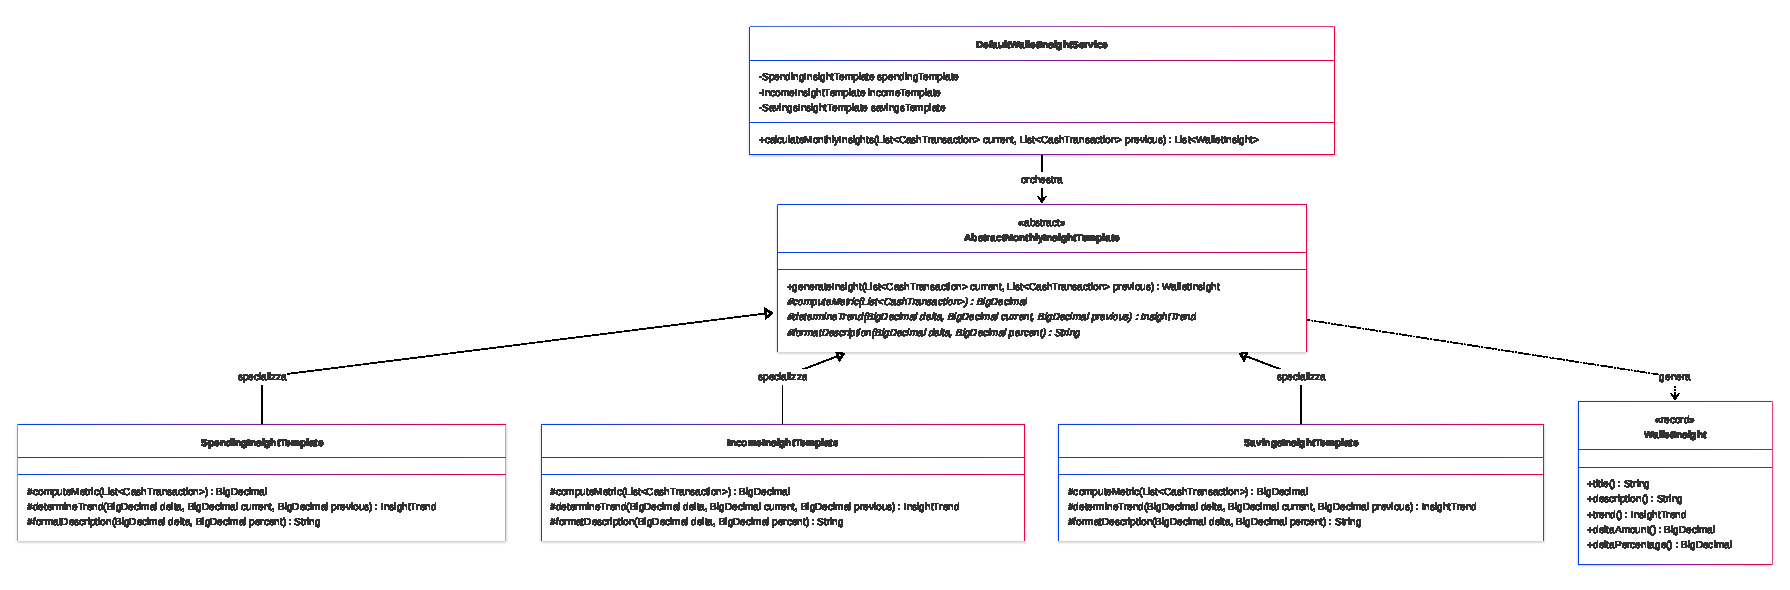
\includegraphics[width=\textwidth]{img/uml-pattern-monthly-insights.png}
\caption{Reificazione del Template Method Pattern per il calcolo comparativo dei Monthly Insights.}
\label{fig:monthly-insights}
\end{figure}

\subsubsection*{4. Pattern utilizzati e reificazione}
\begin{itemize}
    \item \textbf{Template Method Pattern:} Il metodo \texttt{generateInsight()} di \texttt{AbstractMonthlyInsightTemplate} definisce l'ordine di esecuzione immutabile (filtraggio $\rightarrow$ calcolo metriche $\rightarrow$ delta percentuale con gestione divisione per zero $\rightarrow$ determinazione trend).
    \item \textbf{Inversione del Controllo (Hollywood Principle):} Le classi concrete (\texttt{SpendingInsightTemplate}, \texttt{IncomeInsightTemplate}, \texttt{SavingsInsightTemplate}) non controllano il flusso; implementano solo la specifica metrica contabile e la semantica del trend (ad esempio, per le uscite un delta di spesa negativo è un trend \texttt{POSITIVE}, mentre per le entrate è considerato \texttt{NEGATIVE}).
\end{itemize}

\subsection{Filtraggio Composito ed Estendibile della Cronologia (Specification Pattern)}
\subsubsection*{1. Descrizione del problema}
La tabella dei movimenti finanziari della Dashboard mette a disposizione dell'utente una barra di ricerca avanzata con criteri di filtraggio combinabili a piacere:
\begin{itemize}
    \item Intervallo temporale delimitato da data iniziale (\emph{from date}) e finale (\emph{to date});
    \item Tipologia contabile del movimento (\emph{Tutte}, \emph{Solo Entrate}, \emph{Solo Spese}, \emph{Prestiti});
    \item Categoria di spesa o entrata selezionata dal menu a tendina;
    \item Ricerca testuale libera per parola chiave su causale e note descrittive;
    \item Criterio di ordinamento dinamico (cronologico crescente/decrescente o per importo).
\end{itemize}
Una gestione procedurale basata su controlli condizionali concatenati (if-else o cicli mutabili) avrebbe innescato un'esplosione combinatoria ingestibile ($2^4 = 16$ possibili rami logici), rendendo il codice fragile, prono a regressioni e ostico da collaudare nelle singole combinazioni. Inoltre, l'aggiunta di un nuovo parametro di ricerca (ad esempio per importo minimo/massimo) avrebbe costretto a riscrivere la logica interna dell'intero servizio.

\subsubsection*{2. Soluzione proposta e alternative}
\begin{itemize}
    \item \textbf{Alternativa scartata (Filtraggio procedurale con if annidati):} Scartata per la natura non componibile e l'elevata fragilità del flusso imperativo.
    \item \textbf{Alternativa scartata (Predicati Java standard non incapsulati):} L'uso di semplici predicati anonimi (\texttt{Predicate<CashTransaction>}) dispersi nel controller avrebbe privato il dominio di astrazioni formali nominative e riusabili.
    \item \textbf{Soluzione adottata:} Adozione dello Specification Pattern di derivazione Domain-Driven Design. L'interfaccia formale \texttt{TransactionSpecification} estende \texttt{Predicate<CashTransaction>} e implementa metodi di default componibili algebricamente (\texttt{and}, \texttt{or}, \texttt{not}). Attorno a questa radice polimorfica sono state reificate le specifiche atomiche (\texttt{CategoryNameSpecification}, \texttt{CategoryTypeSpecification}, \texttt{DateRangeSpecification}, \texttt{KeywordSpecification}), assemblate in modo compatto dalla factory \texttt{TransactionSpecifications.fromCriteria(criteria)}. Il servizio \texttt{DefaultTransactionHistoryFilterService} riceve i criteri, recupera la specifica composta e filtra lo stream delle transazioni in un singolo passaggio dichiarativo.
\end{itemize}

\subsubsection*{3. Schema UML e Interazioni}
\begin{figure}[H]
\centering
% \includegraphics[width=\textwidth]{img/uml-pattern-transaction-specification.pdf}
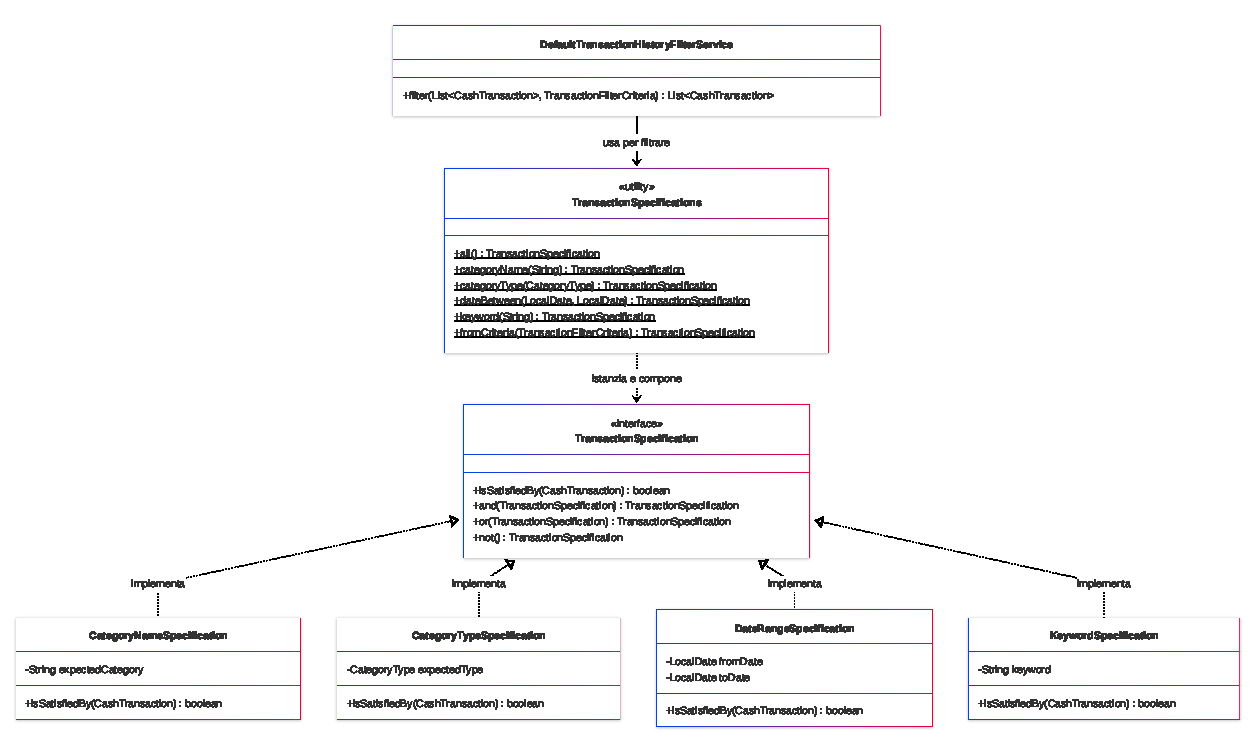
\includegraphics[width=\textwidth]{img/uml-pattern-transaction-specification.png}
\caption{Reificazione dello Specification Pattern per il filtraggio avanzato e componibile delle transazioni.}
\label{fig:transaction-specification}
\end{figure}

\subsubsection*{4. Pattern utilizzati e reificazione}
\begin{itemize}
    \item \textbf{Specification Pattern:} Separa la logica del predicato di business finanziario dall'iterazione sulla collezione; ogni specifica atomica rispetta rigorosamente il principio di singola responsabilità (SRP) ed è testabile in completo isolamento.
    \item \textbf{Factory Method / Combiner:} La classe di utilità \texttt{TransactionSpecifications} centralizza la creazione e la combinazione booleana (\texttt{spec.and(...)}) a partire dal record \texttt{TransactionFilterCriteria}.
    \item \textbf{Functional Pipeline e Defensive Copying:} L'applicazione del filtro sfrutta \texttt{Stream.filter(spec::isSatisfiedBy)} e restituisce liste congelate e immutabili (\texttt{List.copyOf}), proteggendo l'integrità contabile del portafoglio da qualsiasi mutazione esterna.
\end{itemize}

\section{Design Dettagliato (Daniele Zappalà)}

In questa sezione vengono presentati i quattro problemi di progettazione principali affrontati e risolti da \textbf{Daniele Zappalà}, riguardanti la gestione del modulo investimenti, la modellazione degli ordini e delle sorgenti di pagamento, il calcolo continuo di saldi e posizioni dallo storico, il canale di eventi disaccoppiato e la finestra principale con barra laterale condivisa.

\subsection{Ordini con Sorgenti di Pagamento Diverse}

\subsubsection*{1. Descrizione del problema}
Un acquisto di titoli può essere pagato con un conto di liquidità, con una stablecoin posseduta nello stesso conto di investimento, oppure con fondi esterni; lo stesso vale, al contrario, per il ricavato di una vendita. Ogni combinazione modifica conti diversi, e un ordine può fallire per motivi attesi (fondi insufficienti, quantità non posseduta, prezzo non disponibile). La view deve mostrare all'utente un messaggio preciso per ogni caso, e un ordine fallito non deve modificare nessun conto.

\subsubsection*{2. Soluzione proposta e alternative}
La sorgente di pagamento è modellata tramite un'interfaccia sigillata, \texttt{PaymentSource}, con tre implementazioni record: \texttt{CashAccountChannel}, \texttt{StableCoinPositionChannel} e \texttt{NoPaymentChannel}. Anche l'esito di un ordine è un'interfaccia sigillata, \texttt{OrderResult}, con un record per ogni successo (che contiene le transazioni create) e uno per ogni errore (che contiene i dati per spiegarlo, ad esempio importo richiesto e disponibile). \texttt{DefaultInvestmentController} controlla prima che l'ordine sia eseguibile e solo dopo registra le transazioni; nel codice, la scelta tra le sorgenti è gestita tramite uno \texttt{switch} sul tipo con pattern matching, che il compilatore verifica essere esaustivo e completo.

Sono state valutate e scartate tre alternative:
\begin{itemize}
  \item \textbf{Alternativa scartata (Metodi dedicati per combinazione):} Definire un metodo diverso per ogni combinazione di operazione e sorgente avrebbe moltiplicato inutilmente i metodi del controller.
  \item \textbf{Alternativa scartata (Uso di eccezioni):} Ricorrere alle eccezioni per i casi di errore previsto avrebbe appesantito il flusso per situazioni nominali di business, costringendo la view a gestire blocchi \texttt{try-catch} multipli.
  \item \textbf{Alternativa scartata (Parametro generico non tipato):} Passare la sorgente come parametro generico (ad esempio un identificativo di conto) avrebbe disperso controlli \texttt{instanceof} non verificabili dal compilatore.
\end{itemize}
Con i tipi sigillati, l'aggiunta di una nuova sorgente di pagamento obbliga il compilatore a segnalare tutti i punti del codice in cui va gestita.

\subsubsection*{3. Pattern utilizzati e modellazione}
Non si tratta di un pattern GoF tradizionale, bensì della modellazione con tipi sigillati (\emph{sealed interfaces}) e \texttt{record} (tipi algebrici di dati), che consente di trattare successi ed errori come valori ordinari e di sfruttare il pattern matching per switch con verifica statica di esaustività a compile-time.

\subsection{Saldo e Posizioni Calcolati dallo Storico}

\subsubsection*{1. Descrizione del problema}
Il saldo di un conto di liquidità è la somma dei movimenti; quello di un conto di investimento dipende dai prezzi di mercato del momento, e richiede di calcolare per ogni titolo la quantità posseduta, il prezzo medio di carico e il profitto realizzato con le vendite. In entrambi i casi il saldo deve restare coerente con lo storico anche dopo correzioni e cancellazioni.

\subsubsection*{2. Soluzione proposta e alternative}
Il saldo non viene mai memorizzato in modo ridondante. La classe astratta \texttt{AbstractWallet<T extends AbstractTransaction>} contiene lo storico e gestisce tutte le modifiche (aggiunta, rimozione, sostituzione), pubblicando un evento sul bus per ciascuna; il metodo \texttt{getBalance()} è astratto e ogni tipo di conto lo calcola a modo suo. Il parametro generico lega ogni conto al proprio tipo di movimento: il compilatore impedisce a tempo di compilazione di aggiungere un acquisto di titoli a un conto di liquidità, senza richiedere controlli a runtime.

\texttt{InvestmentAccount} raggruppa i movimenti per titolo, ricava le posizioni (\texttt{Position}) con il metodo contabile del costo medio ponderato e delega la richiesta del prezzo corrente a un \texttt{CurrencyConverter}. Il convertitore non viene salvato su file JSON: dopo la fase di caricamento i conti vengono ricollegati mediante il metodo \texttt{withProvider}. Memorizzare saldo e posizioni direttamente nello stato avrebbe reso le letture marginalmente più rapide, ma avrebbe imposto aggiornamenti a catena a ogni variazione dello storico, con alto rischio di disallineamento dei dati.

\subsubsection*{3. Pattern utilizzati e reificazione}
\begin{itemize}
  \item \textbf{Template Method:} \texttt{AbstractWallet} definisce la gestione uniforme dello storico transazioni lasciando astratto il metodo primitivo \texttt{getBalance()}, specializzato rispettivamente da \texttt{CashAccount} e \texttt{InvestmentAccount}.
  \item \textbf{Strategy Pattern:} \texttt{InvestmentAccount} usa un'istanza di \texttt{CurrencyConverter} come strategia intercambiabile per il recupero delle quotazioni correnti, consentendo nei test automatizzati la sostituzione trasparente con un provider a quotazioni prefissate deterministiche.
\end{itemize}

\subsection{Eventi, Tempo dell'Applicazione e Salvataggi Automatici}

\subsubsection*{1. Descrizione del problema}
Più componenti dell'applicazione devono reagire dinamicamente ai cambiamenti dello stato informativo: le viste grafiche devono aggiornarsi, i portafogli vanno persistiti su disco, e per il tracciamento del grafico di andamento il profitto/perdita dei conti di investimento va campionato dopo ogni operazione e a intervalli temporali regolari. Il modello di dominio, tuttavia, deve rimanere disaccoppiato dal toolkit JavaFX, che fornisce i timer sul thread dell'interfaccia.

\subsubsection*{2. Soluzione proposta e alternative}
È stato realizzato un bus di eventi disaccoppiato, \texttt{MessageBus}: i mittenti pubblicano gli eventi senza conoscere i destinatari, e i sottoscrittori specificano la classe di evento d'interesse ricevendo un token per la deregistrazione. Il tempo dell'applicazione è astratto tramite l'interfaccia di dominio \texttt{AppTicker}; la sua implementazione concreta nella view, \texttt{FxAppTicker}, pubblica un \texttt{TickEvent} a intervalli regolari.

\texttt{PeriodicSnapshotSaver} intercetta sia gli eventi di tick temporale sia le transazioni eseguite, salvando un'istantanea di saldo per ciascun conto di investimento a intervalli controllati tramite \texttt{InvestmentsSnapshotService} (su file CSV). Parallelamente, \texttt{WalletAutoSaver} ascolta gli eventi di mutazione e persiste i conti su disco; per ogni tipologia di portafoglio riceve una coppia \texttt{Supplier} / \texttt{Consumer} (lettura e salvataggio), rimanendo completamente agnostico rispetto ai tipi concreti di conto. Prima di questa architettura, la schermata degli investimenti manteneva un timer interno che non veniva rilasciato alla chiusura, provocando duplicazioni ad ogni riapertura.

\subsubsection*{3. Pattern utilizzati e reificazione}
\begin{itemize}
  \item \textbf{Observer Pattern (Publish/Subscribe):} Il \texttt{MessageBus} centralizza la mediazione degli eventi applicativi: i portafogli e \texttt{FxAppTicker} agiscono da publisher, mentre \texttt{PeriodicSnapshotSaver}, \texttt{WalletAutoSaver} e le schermate della GUI operano come subscriber.
  \item \textbf{Strategy Pattern:} L'interfaccia \texttt{InvestmentsSnapshotService} disaccoppia la strategia di memorizzazione delle serie temporali dei conti titoli dall'algoritmo di campionamento.
\end{itemize}

\subsection{Finestra Principale e Barra Laterale Condivisa}

\subsubsection*{1. Descrizione del problema}
La finestra principale (\texttt{MainViewController}) ospita a turno le schermate dei diversi moduli dell'applicazione. La barra laterale di navigazione è unica e condivisa, ma deve visualizzare la lista dei conti pertinente al modulo attivo (portafogli di liquidità o conti titoli) e inoltrare al controller corrispondente le azioni dell'utente (selezione, creazione, rinomina ed eliminazione). Inoltre, le viste aperte si iscrivono a eventi sul bus, e le iscrizioni devono essere revocate tempestivamente alla chiusura per prevenire memory leak.

\subsubsection*{2. Soluzione proposta e alternative}
La barra laterale (\texttt{SideBarViewController}) non mantiene riferimenti diretti ai singoli moduli: interagisce unicamente tramite l'interfaccia formale \texttt{SideBarDelegate}, implementata da ciascuna schermata; al cambio di vista, \texttt{MainViewController} provvede ad aggiornare il delegate corrente. L'aggiunta di un nuovo modulo con conti dedicati richiede unicamente l'implementazione di tale interfaccia.

Tutti i controller delle viste estendono la classe comune \texttt{BaseViewController}, che registra centralmente le sottoscrizioni agli eventi e le rimuove in blocco nel metodo \texttt{dispose()}, invocato dalla finestra principale ad ogni transizione di pagina. I controller JavaFX vengono istanziati dalla factory \texttt{ViewControllersFactory}, che inietta a tempo di costruzione i servizi necessari. L'alternativa scartata (sviluppare barre laterali separate per ciascun modulo) avrebbe generato una cospicua duplicazione di codice e di stili grafici.

\subsubsection*{3. Pattern utilizzati e reificazione}
\begin{itemize}
  \item \textbf{Strategy Pattern (nella variante Delegate):} L'interfaccia \texttt{SideBarDelegate} formalizza la strategia di comunicazione tra la barra laterale e la vista attiva, delegando a quest'ultima l'estrazione dei dati contabili e la gestione dei comandi.
  \item \textbf{Factory Pattern:} La classe \texttt{ViewControllersFactory} accentra la creazione e l'inizializzazione dei controller delle viste con iniezione manuale delle dipendenze applicative.
\end{itemize}


\chapter{Sviluppo}

In questo capitolo vengono presentate le attività di testing automatizzato e le caratteristiche avanzate del linguaggio Java impiegate nello sviluppo del sottosistema assegnato.

\section{Testing Automatizzato}
Il progetto adotta la suite \textbf{JUnit 5} per garantire l'assenza di regressioni e verificare in modo rigoroso e ripetibile la correttezza della logica applicativa.

Per la parte sviluppata da \textbf{Arianna Palmucci}, sono state implementate suite di test unitari e di integrazione esaustive:
\begin{itemize}
    \item \textbf{Motore di Conversione e Precisione Decimale:}
    \begin{itemize}
        \item \texttt{BasicCurrencyConverterTest}: verifica delle conversioni dirette e inverse tra valute fiat.
        \item \texttt{CurrencyConversionResultTest}: verifica del corretto arrotondamento contabile con \texttt{BigDecimal} ed eliminazione degli errori di troncamento.
        \item \texttt{CurrencyConverterTest}: verifica della coerenza delle conversioni tra asset diversi.
    \end{itemize}
    \item \textbf{Provider di Cambio e Caching:}
    \begin{itemize}
        \item \texttt{MockExchangeRateAPITest} e \texttt{ExchangeRateAPIClientTest}: validazione della logica di memorizzazione nella cache e correttezza dei dati di fallback.
        \item \texttt{ExchangeRateTest}: verifica delle invarianti numeriche delle quotazioni.
    \end{itemize}
    \item \textbf{Simulazioni Bancarie e Commissioni:}
    \begin{itemize}
        \item \texttt{BankTest}, \texttt{BankCalculatorTest}, \texttt{BankConversionResultTest}, \texttt{BankServiceTest}: verifica rigorosa delle commissioni fisse, percentuali e spread bid/ask per istituti di credito simulati.
    \end{itemize}
    \item \textbf{Allerte di Mercato e Watchlist:}
    \begin{itemize}
        \item \texttt{CurrencyAlertTest}, \texttt{CurrencyAlertServiceTest}, \texttt{MarketAlertViewTest}: verifica delle condizioni di innesco delle allerte su soglie di prezzo.
        \item \texttt{WatchListTest}, \texttt{WatchlistPairTest}: verifica dell'unicità e della gestione della lista di osservazione.
    \end{itemize}
    \item \textbf{Preferenze, Temi e Memento:}
    \begin{itemize}
        \item \texttt{SettingsTest}, \texttt{SettingsSnapshotTest}: verifica della creazione, archiviazione e ripristino degli snapshot di configurazione.
        \item \texttt{SettingsManagerTest}: test di persistenza e deserializzazione del file JSON delle impostazioni.
        \item \texttt{ThemeTest}, \texttt{WindowPreferencesTest}, \texttt{ThemeManagerTest}: verifica della propagazione dei temi e salvataggio delle coordinate geometriche della finestra.
    \end{itemize}
\end{itemize}

Per la parte sviluppata da \textbf{Daniele Zappalà}, le attività di testing automatizzato coprono il modulo investimenti, i contratti di esecuzione degli ordini e le componenti infrastrutturali:
\begin{itemize}
    \item \textbf{Investimenti e Rendicontazione Portafoglio Titoli:}
    \begin{itemize}
        \item \texttt{InvestmentAccountTest}: verifica del calcolo delle posizioni contabili, del prezzo medio ponderato di carico, del profitto/perdita non realizzato e del profitto realizzato a fronte di vendite parziali.
        \item \texttt{DefaultInvestmentControllerTest}: collaudo esaustivo degli ordini di acquisto, vendita e trasferimento con tutte le sorgenti di pagamento (\texttt{PaymentSource}), gestendo sia gli esiti nominali sia le condizioni anomale (fondi insufficienti, disponibilità titoli carente, conversioni tra valute diverse).
        \item \texttt{InvestmentAccountPersistenceTest}: test di persistenza e ricaricamento da file JSON con conservazione dell'identificativo UUID.
    \end{itemize}
    \item \textbf{Campionamento Temporale e Fonti Dati:}
    \begin{itemize}
        \item \texttt{PeriodicSnapshotSaverTest}: verifica del salvataggio periodico delle istantanee temporali mediante ticker simulato deterministico.
        \item \texttt{CryptoPriceBatchTest}: test di deserializzazione delle quotazioni da payload memorizzati, compresa la gestione di rate limit e quote esaurite.
    \end{itemize}
\end{itemize}

Tutti i test vengono eseguiti automaticamente dal task \texttt{./gradlew check}. Il codice rispetta rigorosamente i controlli statici di Checkstyle, PMD e SpotBugs con zero violazioni.

\section{Note di Sviluppo}

\subsection{Favour Emuwahen}

Di seguito viene fornito l'elenco analitico delle feature avanzate del linguaggio Java (versione 21 LTS) e delle librerie applicative impiegate nello sviluppo del sottosistema Dashboard e Contabilità, corredate da specifici riferimenti e permalink al repository GitHub nel branch \texttt{base}:

\begin{itemize}
    \item \textbf{Gerarchie Sigillate ed Ereditarietà Controllata (\emph{sealed classes}):} Utilizzo di classi astratte sigillate (\texttt{public abstract sealed class AbstractTransaction permits CashTransaction, InvestmentTransaction}) per delimitare a compile-time l'albero polimorfico delle transazioni monetarie, abilitando controlli di esaustività ed escludendo estensioni non autorizzate.
    \begin{itemize}
        \item \emph{Riferimento:} \url{https://github.com/leoI0II/OOP25-UniBodget/blob/base/app/src/main/java/it/unibo/unibodget/model/transactions/base/AbstractTransaction.java}
    \end{itemize}

    \item \textbf{Progettazione con Interfacce Funzionali e Generici Componibili (\texttt{Predicate\textless T\textgreater}):} L'interfaccia di specifica estende \texttt{Predicate\textless CashTransaction\textgreater} e implementa metodi di default componibili algebricamente (\texttt{and}, \texttt{or}, \texttt{not}) tramite espressioni lambda.
    \begin{itemize}
        \item \emph{Riferimento:} \url{https://github.com/leoI0II/OOP25-UniBodget/blob/base/app/src/main/java/it/unibo/unibodget/model/dashboard/specification/TransactionSpecification.java}
    \end{itemize}

    \item \textbf{Pattern Matching per Switch e Record Patterns (Java 21):} Utilizzo del pattern matching per switch con decostruzione dei record (\texttt{case PaymentSource.NoPaymentChannel() -\textgreater \dots}) all'interno dei selettori di stato e di pagamento, eliminando cast manuali e variabili locali inutilizzate.
    \begin{itemize}
        \item \emph{Riferimento:} \url{https://github.com/leoI0II/OOP25-UniBodget/blob/base/app/src/main/java/it/unibo/unibodget/view/dashboard/impl/NewTransactionDialog.java}
    \end{itemize}

    \item \textbf{Records Immutabili per il Trasferimento Dati (\emph{Data Transfer Objects}):} Definizione di record nativi per modellare lo stato di presentazione della UI (\texttt{DashboardViewState}, \texttt{HeaderCardState}, \texttt{BalanceCardState}, \texttt{BudgetCardState}) e le strutture di richiesta (\texttt{NewTransactionRequest}, \texttt{BudgetStatus}, \texttt{WalletInsight}), garantendo immutabilità strutturale e azzerando il codice boilerplate.
    \begin{itemize}
        \item \emph{Riferimento:} \url{https://github.com/leoI0II/OOP25-UniBodget/blob/base/app/src/main/java/it/unibo/unibodget/view/dashboard/state/DashboardViewState.java}
    \end{itemize}

    \item \textbf{Stream API Avanzate e Pipeline di Riduzione Funzionale (\texttt{Collectors.groupingBy}):} Elaborazione dello storico transazioni mediante pipeline con operatori intermedi e terminali (\texttt{.filter()}, \texttt{.map()}, \texttt{.sorted()}, \texttt{.reduce()}) per il calcolo dei saldi cumulativi (\texttt{BigDecimal.ZERO}, \texttt{BigDecimal::add}) e raggruppamento delle spese con \texttt{Collectors.groupingBy()} in \texttt{DefaultCategoryService}.
    \begin{itemize}
        \item \emph{Riferimento:} \url{https://github.com/leoI0II/OOP25-UniBodget/blob/base/app/src/main/java/it/unibo/unibodget/model/dashboard/impl/DefaultCategoryService.java}
    \end{itemize}

    \item \textbf{Aritmetica Decimale Esatta (\texttt{java.math.BigDecimal}) e Arrotondamento Finanziario:} Rappresentazione e calcolo rigoroso di tutti gli importi, percentuali di budget e tassi di variazione mese su mese con \texttt{BigDecimal} e arrotondamento bancario controllato (\texttt{RoundingMode.HALF\_UP}), eliminando gli errori di approssimazione dell'aritmetica floating-point IEEE 754.
    \begin{itemize}
        \item \emph{Riferimento:} \url{https://github.com/leoI0II/OOP25-UniBodget/blob/base/app/src/main/java/it/unibo/unibodget/model/dashboard/impl/AbstractMonthlyInsightTemplate.java}
    \end{itemize}

    \item \textbf{Pattern Creazionale Builder Fluente con Validazione delle Invarianti:} Costruzione atomica di oggetti complessi con controllo a tempo di creazione dei vincoli di consistenza contabile (es. obbligatorietà del campo \texttt{friendName} per transazioni di tipo \texttt{FRIEND\_LOAN}).
    \begin{itemize}
        \item \emph{Riferimento:} \url{https://github.com/leoI0II/OOP25-UniBodget/blob/base/app/src/main/java/it/unibo/unibodget/model/transactions/base/CashTransaction.java}
    \end{itemize}

    \item \textbf{Disaccoppiamento ad Eventi con MessageBus:} Architettura orientata agli eventi per la sincronizzazione dei componenti attraverso la pubblicazione e sottoscrizione disaccoppiata di eventi applicativi (\texttt{TransactionAddedEvent}).
    \begin{itemize}
        \item \emph{Riferimento:} \url{https://github.com/leoI0II/OOP25-UniBodget/blob/base/app/src/main/java/it/unibo/unibodget/model/utils/MessageBus.java}
    \end{itemize}

    \item \textbf{Architettura GUI Modulare in JavaFX 21 con Passive View:} Separazione netta tra logica di presentazione e rendering visuale, con controller snelli che manipolano unicamente lo stato della vista e delegano il layout ai componenti grafici.
    \begin{itemize}
        \item \emph{Riferimento:} \url{https://github.com/leoI0II/OOP25-UniBodget/blob/base/app/src/main/java/it/unibo/unibodget/controller/dashboard/impl/DefaultDashboardController.java}
    \end{itemize}
\end{itemize}

\subsection{Arianna Palmucci}

Di seguito si riportano le caratteristiche avanzate del linguaggio Java 21 LTS e dell'ecosistema applicativo impiegate nello sviluppo del modulo di gestione delle valute, motore di conversione, persistenza, temi e preferenze dell'applicazione, corredate dai rispettivi riferimenti e permalink al codice sorgente nel branch \texttt{base}:

\begin{itemize}
    \item \textbf{Polimorfismo Valutario, Gerarchie Eterogenee e Tipizzazione Forte:}
    \begin{itemize}
        \item Definizione dell'interfaccia radice comune \texttt{CurrencyUnit} implementata in modo polimorfico da enumerazioni distinte per tipologia finanziaria (\texttt{FiatCurrency}, \texttt{CryptoCurrency}, \texttt{StockMarketCurrency}) e dalla classe estendibile \texttt{Currency}.
        \item \emph{Riferimento:} \url{https://github.com/leoI0II/OOP25-UniBodget/blob/base/app/src/main/java/it/unibo/unibodget/model/currency/CurrencyUnit.java}
    \end{itemize}

    \item \textbf{Interfacce Funzionali e Callback Reattive (\texttt{java.util.function.*}):}
    \begin{itemize}
        \item Utilizzo esteso di \texttt{Consumer\textless T\textgreater}, \texttt{Function\textless T, R\textgreater} e \texttt{BiFunction\textless T, U, R\textgreater} nei controller e nelle viste per una programmazione dichiarativa e reattiva.
        \item \emph{Riferimento:} \url{https://github.com/leoI0II/OOP25-UniBodget/blob/base/app/src/main/java/it/unibo/unibodget/model/currency/alert/CurrencyAlertService.java}
    \end{itemize}

    \item \textbf{Stream API, Pipeline Funzionali e Costrutto \texttt{Optional}:}
    \begin{itemize}
        \item Adozione sistematica di \texttt{Optional\textless BigDecimal\textgreater} e \texttt{OptionalDouble} nella classe \texttt{MonetaryInputParser} per prevenire eccezioni non controllate e azzerare l'uso di riferimenti \texttt{null}.
        \item Elaborazione dichiarativa delle collezioni di tassi, filtraggio delle allerte e trasformazioni di liste valutarie tramite pipeline (\texttt{.filter()}, \texttt{.map()}, \texttt{.toList()}).
        \item \emph{Riferimento:} \url{https://github.com/leoI0II/OOP25-UniBodget/blob/base/app/src/main/java/it/unibo/unibodget/model/currency/MonetaryInputParser.java}
    \end{itemize}

    \item \textbf{Java Time API (\texttt{java.time.*}):}
    \begin{itemize}
        \item Gestione temporale immutabile con \texttt{Instant}, \texttt{Duration} e \texttt{LocalDate} per la scadenza della cache in-memory e l'ordinamento cronologico delle serie storiche dei tassi di cambio.
        \item \emph{Riferimento:} \url{https://github.com/leoI0II/OOP25-UniBodget/blob/base/app/src/main/java/it/unibo/unibodget/model/currency/api/ExchangeRateAPIClient.java}
    \end{itemize}

    \item \textbf{Modern HTTP Client (\texttt{java.net.http.*}):}
    \begin{itemize}
        \item Utilizzo di \texttt{HttpClient} e \texttt{HttpRequest} con supporto nativo HTTP/2, timeout dedicati (\texttt{Duration.ofSeconds(10)}) e gestione resiliente delle chiamate RESTful verso i servizi web di quotazione.
        \item \emph{Riferimento:} \url{https://github.com/leoI0II/OOP25-UniBodget/blob/base/app/src/main/java/it/unibo/unibodget/model/currency/api/ExchangeRateAPIClient.java}
    \end{itemize}

    \item \textbf{Serializzazione e Deserializzazione JSON Avanzata con Jackson (\texttt{com.fasterxml.jackson}):}
    \begin{itemize}
        \item Configurazione centralizzata di \texttt{ObjectMapper} con modulo \texttt{JavaTimeModule} e deserializzatori custom per la ricostruzione polimorfica di \texttt{CurrencyUnit} tramite factory method \texttt{CurrencyUnit.getByCode(code)} e persistenza di \texttt{Settings}, \texttt{BankList}, \texttt{ThemeList} e \texttt{WatchList}.
        \item \emph{Riferimento:} \url{https://github.com/leoI0II/OOP25-UniBodget/blob/base/app/src/main/java/it/unibo/unibodget/model/settings/SettingsManager.java}
    \end{itemize}

    \item \textbf{Java NIO.2 e Gestione Resiliente del File System (\texttt{java.nio.file.*}):}
    \begin{itemize}
        \item Manipolazione robusta di percorsi e file mediante \texttt{Path}, \texttt{Files.exists()}, \texttt{Files.createDirectories()} e \texttt{Files.copy(InputStream, Path)} in \texttt{AppDataPathResolver} per garantire l'indipendenza dalla piattaforma OS.
        \item \emph{Riferimento:} \url{https://github.com/leoI0II/OOP25-UniBodget/blob/base/app/src/main/java/it/unibo/unibodget/persistency/AppDataPathResolver.java}
    \end{itemize}

    \item \textbf{JavaFX 21 Avanzato: Scomposizione Modulare, Grafici e CSS Dinamico:}
    \begin{itemize}
        \item Realizzazione di widget modulari e componibili, grafici storici \texttt{LineChart} e iniezione a runtime dei fogli di stile con gestione dinamica dei temi chiaro/scuro in \texttt{ThemeManager}.
        \item \emph{Riferimento:} \url{https://github.com/leoI0II/OOP25-UniBodget/blob/base/app/src/main/java/it/unibo/unibodget/model/settings/ThemeManager.java}
    \end{itemize}

    \item \textbf{Robustezza Numerica con \texttt{BigDecimal} e Precisione Finanziaria:}
    \begin{itemize}
        \item Impiego sistematico di \texttt{BigDecimal} con scala esplicita e \texttt{RoundingMode.HALF\_UP} per prevenire qualsiasi errore di cancellazione numerica o imprecisione nei calcoli di conversione monetaria e commissioni bancarie.
        \item \emph{Riferimento:} \url{https://github.com/leoI0II/OOP25-UniBodget/blob/base/app/src/main/java/it/unibo/unibodget/model/currency/engin/CurrencyConverter.java}
    \end{itemize}

    \item \textbf{Pattern Matching, Records Immutabili e Costrutti Moderni di Java 21:}
    \begin{itemize}
        \item Definizione di record immutabili per il trasferimento dati (\texttt{CurrencyConversionResult}, \texttt{Bank}) e pattern matching per switch per un codice conciso ed esente da boilerplate.
        \item \emph{Riferimento:} \url{https://github.com/leoI0II/OOP25-UniBodget/blob/base/app/src/main/java/it/unibo/unibodget/model/currency/CurrencyConversionResult.java}
    \end{itemize}
\end{itemize}

\subsection{Daniele Zappalà}

Di seguito si riportano le caratteristiche avanzate del linguaggio Java (versione 21 LTS) e le librerie utilizzate per lo sviluppo del modulo investimenti, del bus di eventi e dell'infrastruttura condivisa, corredate dai rispettivi permalink:

\begin{itemize}
  \item \textbf{Interfacce \texttt{sealed} e \texttt{record} per modellare le sorgenti di pagamento}\\
    \url{https://github.com/leoI0II/OOP25-UniBodget/blob/dcf7b2c11de58754a6b6dd15155276ac9113b07a/app/src/main/java/it/unibo/unibodget/model/investment/PaymentSource.java#L23-L52}
  \item \textbf{Pattern matching nello \texttt{switch} su tipi sigillati}\\
    \url{https://github.com/leoI0II/OOP25-UniBodget/blob/dcf7b2c11de58754a6b6dd15155276ac9113b07a/app/src/main/java/it/unibo/unibodget/model/investment/controllers/DefaultInvestmentController.java#L511-L521}
  \item \textbf{Metodo generico con tipo limitato e \emph{type token} (\texttt{<T extends MessageEvent>})}\\
    \url{https://github.com/leoI0II/OOP25-UniBodget/blob/dcf7b2c11de58754a6b6dd15155276ac9113b07a/app/src/main/java/it/unibo/unibodget/model/utils/MessageBus.java#L59-L66}
  \item \textbf{Metodo generico con interfacce funzionali (\texttt{Supplier}, \texttt{Consumer})}\\
    \url{https://github.com/leoI0II/OOP25-UniBodget/blob/dcf7b2c11de58754a6b6dd15155276ac9113b07a/app/src/main/java/it/unibo/unibodget/persistency/WalletAutoSaver.java#L59-L80}
  \item \textbf{Stream con \texttt{Collectors.groupingBy} per calcolare le posizioni}\\
    \url{https://github.com/leoI0II/OOP25-UniBodget/blob/dcf7b2c11de58754a6b6dd15155276ac9113b07a/app/src/main/java/it/unibo/unibodget/model/wallet/InvestmentAccount.java#L146-L160}
  \item \textbf{\texttt{Optional} e \texttt{Comparator} con method reference (miglior e peggior titolo)}\\
    \url{https://github.com/leoI0II/OOP25-UniBodget/blob/dcf7b2c11de58754a6b6dd15155276ac9113b07a/app/src/main/java/it/unibo/unibodget/model/investment/controllers/DefaultInvestmentController.java#L667-L677}
  \item \textbf{Reflection per creare i controller delle pagine FXML}\\
    \url{https://github.com/leoI0II/OOP25-UniBodget/blob/dcf7b2c11de58754a6b6dd15155276ac9113b07a/app/src/main/java/it/unibo/unibodget/view/main/ViewControllersFactory.java#L64-L90}
  \item \textbf{API \texttt{java.time} (\texttt{ChronoUnit}) per il formato delle date del grafico}\\
    \url{https://github.com/leoI0II/OOP25-UniBodget/blob/dcf7b2c11de58754a6b6dd15155276ac9113b07a/app/src/main/java/it/unibo/unibodget/view/investments/InvestmentsViewController.java#L274-L286}
  \item \textbf{Metodo generico con lambda per le colonne numeriche delle tabelle JavaFX}\\
    \url{https://github.com/leoI0II/OOP25-UniBodget/blob/dcf7b2c11de58754a6b6dd15155276ac9113b07a/app/src/main/java/it/unibo/unibodget/view/investments/InvestmentsViewController.java#L382-L400}
  \item \textbf{Libreria Apache Commons CSV per le istantanee del profitto/perdita}\\
    \url{https://github.com/leoI0II/OOP25-UniBodget/blob/dcf7b2c11de58754a6b6dd15155276ac9113b07a/app/src/main/java/it/unibo/unibodget/model/investment/service/CSVInvestmentsSnapshotService.java#L151-L170}
  \item \textbf{Libreria JavaFX: \texttt{Timeline} per il tempo dell'applicazione}\\
    \url{https://github.com/leoI0II/OOP25-UniBodget/blob/dcf7b2c11de58754a6b6dd15155276ac9113b07a/app/src/main/java/it/unibo/unibodget/view/utils/FxAppTicker.java#L29-L40}
\end{itemize}

\chapter{Commenti finali}

\section{Autovalutazione e lavori futuri}

\subsection{Favour Emuwahen}
All'interno del progetto UniBodget mi sono occupato della progettazione architetturale, dello sviluppo e del collaudo del sottosistema Dashboard, della gestione dei Portafogli di Cassa (\emph{Cash Accounts}), del ciclo di vita delle Transazioni Contanti (\emph{Cash Transactions}), del monitoraggio del Budget, del motore di analisi statistica dei Trend Mensili (\emph{Monthly Insights}) e del motore di filtraggio avanzato con lo Specification Pattern.

\subsubsection*{Punti di forza del contributo:}
\begin{itemize}
    \item \textbf{Solidità architetturale e applicazione rigorosa dei design pattern:} L'adozione coordinata di pattern creazionali (Builder, Factory Method), comportamentali (Template Method, Specification, Strategy) e strutturali (Facade, Passive View) ha reso il codice modulare, orientato all'estendibilità futura senza violare il principio Open-Closed (OCP).
    \item \textbf{Integrità contabile e immutabilità:} Nessuna transazione può essere generata in uno stato parziale o incoerente grazie alle invarianti verificate a tempo di costruzione nel Builder. Tutti i calcoli patrimoniali operano con aritmetica esatta \texttt{BigDecimal} e arrotondamento bancario controllato (\texttt{RoundingMode.HALF\_UP}).
    \item \textbf{Qualità formale del codice e conformità QA:} Conseguimento di 0 violazioni statiche secondo il severo profilo imposto da \texttt{gradle-java-qa} (Checkstyle, PMD e SpotBugs), con totale rimozione di numeri magici di layout, copie difensive e incapsulamento rigoroso.
    \item \textbf{Copertura di test esaustiva:} Realizzazione di una suite di oltre 15 classi di test automatici con JUnit 5 con un tasso di successo del 100\%, verificando sia i casi nominali sia le condizioni al contorno (divisione per zero, transazioni prive di categoria, vincoli sui prestiti).
\end{itemize}

\subsubsection*{Punti di debolezza ed elementi migliorabili:}
\begin{itemize}
    \item \textbf{Sincronizzazione asincrona:} Le operazioni di ricalcolo della dashboard e di salvataggio dello snapshot vengono attualmente eseguite in modo sincrono sul thread chiamante; l'introduzione di \texttt{CompletableFuture} per il recupero concorrente delle statistiche mensili avrebbe ulteriormente ottimizzato i tempi di caricamento su collezioni storiche di dimensioni molto elevate.
    \item \textbf{Conversione multivaluta omnicomprensiva nel cruscotto:} Attualmente la dashboard calcola il saldo aggregato aggregando le transazioni appartenenti al portafoglio nella sua valuta base specifica; una conversione istantanea incrociata omnicomprensiva su tutte le valute mondiali nella vista principale arricchirebbe ulteriormente l'esperienza d'uso.
\end{itemize}

\subsubsection*{Ruolo all'interno del gruppo:}
All'interno del team ho curato la progettazione e l'implementazione del cuore funzionale dell'applicazione: il sottosistema Dashboard, il motore delle transazioni di cassa, il monitoraggio delle soglie di spesa e l'integrazione del sistema di visualizzazione grafica. Ho inoltre coordinato la definizione dei contratti di interfaccia DTO (tramite Java Records) che hanno permesso ai colleghi di lavorare in parallelo senza interferenze sui rispettivi moduli.

\subsubsection*{Sviluppi futuri:}
Qualora il progetto venisse proseguito per una distribuzione aperta, le direttrici evolutive più promettenti includono:
\begin{enumerate}
    \item \textbf{Budgeting predittivo intelligente:} Integrazione di modelli statistici o di machine learning leggero per prevedere l'andamento delle spese a fine mese sulla base dello storico dei consumi settimanali.
    \item \textbf{Esportazione contabile avanzata:} Generazione automatica di rendiconti periodici e prospetti fiscali in formato PDF vettoriale, CSV RFC 4180 ed Excel.
    \item \textbf{Sincronizzazione Cloud sicura:} Espansione del layer di persistenza locale verso un'architettura ibrida con replica cifrata dei dati su cloud storage personale.
\end{enumerate}

\subsection{Arianna Palmucci}

All'interno del progetto UniBodget mi sono occupata della progettazione architetturale, dello sviluppo e del collaudo del sottosistema Valute e Mercato, del motore di Conversione Monetaria (\emph{Currency Converter}), dell'integrazione del client di rete per i tassi di cambio esterni con gestione della cache e fallback offline, del monitoraggio e notifica delle Allerte Valutarie (\emph{Currency Alerts}), del sistema di gestione persistente delle Watchlist, delle Banche e delle Impostazioni utente (\emph{Settings}), nonché dell'infrastruttura di tematizzazione grafica dinamica (\emph{Theme Manager}) e della validazione centralizzata dell'input monetario (\emph{Monetary Input Parser}).

\subsubsection*{Punti di forza del contributo:}
\begin{itemize}
    \item \textbf{Modularità e separazione delle responsabilità:} Disaccoppiamento netto tra il modello matematico di conversione, le fonti remote dei tassi e l'interfaccia grafica. La vista del convertitore è stata scomposta in widget modulari specializzati e riutilizzabili (\texttt{ConverterWidgetFX}, \texttt{BankConverterWidgetFX}, \texttt{CurrencyHistoryChartView}, \texttt{WatchlistWidgetFX}).
    \item \textbf{Resilienza e tolleranza ai guasti di rete:} Progettazione di un'architettura di rete a doppio livello con caching intelligente in-memory (TTL configurabile) e meccanismo trasparente di fallback: qualora le API esterne di borsa non siano raggiungibili, il convertitore continua a funzionare regolarmente sui tassi memorizzati nella cache o sui tassi predefiniti, garantendo la totale continuità di servizio.
    \item \textbf{Precisione numerica e validazione robusta (\emph{Single Source of Truth}):} Centralizzazione delle logiche di parsing e sanificazione dell'input numerico monetario nella classe \texttt{MonetaryInputParser}, gestendo uniformemente separatori decimali italiani e anglosassoni, importi negativi e formati non validi con tipi di ritorno sicuri (\texttt{Optional\textless BigDecimal\textgreater}). Tutti i calcoli di cambio e commissione adottano aritmetica esatta \texttt{BigDecimal} con arrotondamento bancario.
    \item \textbf{Persistenza JSON strutturata e dinamica dei temi:} Adozione del pattern Memento per il salvataggio atomico delle impostazioni utente su file JSON in directory sandbox OS-independent, associata all'iniezione dinamica a runtime dei fogli di stile CSS per il cambio tema istantaneo chiaro/scuro su tutta la scena applicativa.
    \item \textbf{Qualità formale del codice e copertura di test:} Totale conformità ai controlli di analisi statica di Checkstyle, PMD e SpotBugs con zero violazioni; realizzazione di una suite di test unitari automatizzati completa con JUnit 5 per verificare conversioni triangolari, soglie di allerta, parsing numerico e persistenza JSON.
\end{itemize}

\subsubsection*{Punti di debolezza ed elementi migliorabili:}
\begin{itemize}
    \item \textbf{Molteplicità di provider API remoti:} Attualmente il sistema integra un singolo provider di cambio valute primario via HTTP; l'introduzione di una catena di responsabilità (\emph{Chain of Responsibility}) con provider secondari alternativi (es. CoinGecko per crypto, Yahoo Finance per azioni) avrebbe aumentato ulteriormente la ridondanza.
    \item \textbf{Aggiornamento dei tassi storici in background concorrente:} Il recupero dei grafici storici su ampi intervalli temporali viene richiamato su richiesta; un job di sincronizzazione asincrono schedulato in background ridurrebbe la latenza percepita al primo accesso al grafico.
\end{itemize}

\subsubsection*{Ruolo all'interno del gruppo:}
All'interno del team ho curato la definizione delle basi del dominio multivaluta (interfaccia \texttt{CurrencyUnit} e relative implementazioni), l'intero ecosistema di quotazione e conversione monetaria, il layer di persistenza, la gestione delle preferenze dell'applicazione e la coerenza visiva dell'interfaccia grafica tramite l'architettura dei temi. Ho inoltre collaborato attivamente alla definizione dell'architettura MVC comune, all'integrazione del MessageBus tra i vari moduli e alla gestione accurata delle finestre modali e popup di dialogo (\texttt{SettingsPopupFX}, grafici storici e dialoghi di allerta), garantendo che ogni schermata secondaria si apra effettivamente come una vera finestra popup sopraelevata e contestuale anziché essere gestita come una visualizzazione a schermo intero.

\subsubsection*{Sviluppi futuri:}
Qualora il progetto venisse proseguito per una distribuzione aperta, le direttrici evolutive più promettenti includono:
\begin{enumerate}
    \item \textbf{Supporto a provider multipli concorrenti con fallback a cascata:} Implementazione di strategie adattive di selezione della fonte di cambio con bilanciamento del carico tra endpoint pubblici gratuiti.
    \item \textbf{Ottimizzatore avanzato delle commissioni bancarie:} Algoritmo di confronto automatico multicriterio tra le banche censite per suggerire all'utente l'istituto finanziario più conveniente in base all'importo e alla valuta scambiata.
    \item \textbf{Basket valutario personalizzato e indici sintetici:} Possibilità per l'utente di creare panieri di valute o indici compositi su misura per monitorare in tempo reale il valore ponderato del proprio portafoglio internazionale.
    \item \textbf{Filtri di ordinamento come varianti intercambiabili:} Estendere i criteri di ordinamento dell'elenco contabile (per data, importo o categoria) strutturandoli come varianti del pattern Strategy, garantendo flessibilità e combinazione fluida con i filtri esistenti.
    \item \textbf{Persistenza evoluta con servizi e cloud storage esterni:} Integrare provider remoti (es. Google Drive, Dropbox o cloud storage cifrati) per il salvataggio dei dati contabili e delle impostazioni, assicurando backup automatico e sincronizzazione trasparente multi-device.
    \item \textbf{Ottimizzazione responsive degli spazi per l'elenco transazioni:} Rifinire la vista tabellare delle transazioni con layout ad auto-adattamento e scorrimento virtualizzato, massimizzando la leggibilità dei record contabili anche a risoluzioni ridotte o su finestre compatte.
    \item \textbf{Micro-interazioni visive, effetti mouse over e feedback UI:} Arricchire l'interfaccia JavaFX con transizioni fluide, evidenziazioni cromatiche al passaggio del mouse (\emph{mouse hover}) su pulsanti e righe e tooltip dinamici riepilogativi su grafici e tabelle.
    \item \textbf{Ecosistema multipiattaforma (Database, Server, Web e Mobile):} Progettare un'infrastruttura client-server scalabile con database relazionale/NoSQL e API REST, affiancando all'applicativo desktop un portale web responsivo e un'app mobile per la gestione in mobilità.
    \item \textbf{Refactoring architetturale continuo e Dependency Injection:} Perfezionare costantemente il disaccoppiamento tra controller e logica di dominio mediante Dependency Injection (es. Guice) e separazione formale dei contratti di servizio, elevando la manutenibilità del codice.
\end{enumerate}

\subsection{Daniele Zappalà}

All'interno del progetto UniBodget mi sono occupato della progettazione, sviluppo e collaudo del modulo degli investimenti: conti di investimento (\texttt{InvestmentAccount}), calcolo continuo di posizioni e profitto/perdita, ordini di acquisto, vendita e trasferimento titoli con le diverse sorgenti di pagamento (\texttt{PaymentSource}), istantanee periodiche temporali (\texttt{BalanceSnapshot}), grafico di andamento e pagina \emph{Portfolio}. Ho inoltre realizzato la finestra principale (\texttt{MainViewController}) con la barra laterale condivisa con pattern Delegate, in cui sono integrate a runtime le pagine degli altri moduli, il canale disaccoppiato di eventi (\texttt{MessageBus}), il tempo dell'applicazione (\texttt{AppTicker}) e il sottosistema di salvataggio automatico dei portafogli (\texttt{WalletAutoSaver}). Nel team ho curato inoltre buona parte dell'integrazione tra i moduli e la convergenza dei rami di sviluppo.

\subsubsection*{Punti di forza del contributo:}
\begin{itemize}
  \item \textbf{Tipi sigillati per ordini ed esiti contabili:} Le sorgenti di pagamento e gli esiti degli ordini sono modellati tramite interfacce sigillate (\texttt{PaymentSource}, \texttt{OrderResult}): il compilatore verifica a tempo di compilazione l'esaustività dello \texttt{switch}, e gli errori previsti giungono alla view come strutture dati descrittive, eliminando eccezioni e logiche imperativo-procedurali.
  \item \textbf{Integrità contabile e ricalcolo dallo storico:} Saldi, posizioni e profitto/perdita sono sempre calcolati a partire dallo storico delle transazioni con metodo contabile a costo medio ponderato, garantendo coerenza anche dopo modifiche o cancellazioni retroattive.
  \item \textbf{Disaccoppiamento del model da JavaFX:} Il modello degli investimenti non dipende dal toolkit grafico; anche il tempo dell'applicazione è un'astrazione del model (\texttt{AppTicker}), implementata nella view tramite \texttt{FxAppTicker}.
  \item \textbf{Copertura di test e determinismo:} Il controller degli investimenti e i conti sono coperti da test approfonditi su tutte le combinazioni di operazioni e sorgenti di pagamento, adottando convertitori deterministici a quotazioni fisse indipendenti dalla rete.
\end{itemize}

\subsubsection*{Punti di debolezza ed elementi migliorabili:}
\begin{itemize}
  \item \textbf{Canale eventi statico:} Il \texttt{MessageBus} adotta un pattern statico, rendendolo unico per l'intera applicazione. Sebbene pratico, in fase di test automatizzati indipendenti gli iscritti vengono condivisi tra test diversi; un'istanza iniettata tramite costruttore avrebbe garantito un isolamento superiore.
  \item \textbf{Ricalcolo retroattivo delle istantanee:} Le istantanee di portafoglio già salvate su CSV non vengono ricalcolate retroattivamente quando si modifica o elimina una transazione passata, lasciando discrepanze temporali sullo storico del grafico per quel dato intervallo.
  \item \textbf{Risoluzione sincrona dei prezzi:} La risoluzione dei prezzi correnti avviene sul thread chiamante: al primo accesso alla pagina degli investimenti, se le quotazioni non sono ancora in memoria, si può verificare una breve latenza visiva.
\end{itemize}

\subsubsection*{Sviluppi futuri:}
\begin{enumerate}
  \item \textbf{Caricamento asincrono delle quotazioni:} Recupero dei prezzi di mercato in background con \texttt{CompletableFuture} per azzerare i tempi di attesa al primo avvio della vista.
  \item \textbf{Personalizzazione temporale e analitica dei grafici:} Introduzione nel grafico di performance della selezione dinamica dell'intervallo temporale (giorno, settimana, mese, anno) e grafici di andamento per i singoli titoli in portafoglio.
  \item \textbf{Ricalcolo dinamico degli snapshot:} Algoritmo di rigenerazione trasparente delle istantanee storiche a seguito di modifiche o eliminazioni retroattive di transazioni contabili.
  \item \textbf{Evoluzione Web Multi-utente e Multi-tenant:} In una futura estensione web con autenticazione utente, evolvere il \texttt{MessageBus} da singleton statico a istanza con scope di sessione utente, affiancando un database relazionale per la persistenza multi-utente e riusando l'intero Model e i Controller agnostici dalla GUI.
\end{enumerate}


\section{Difficoltà Incontrate e Commenti per i Docenti}

Nel corso del progetto, il team ha affrontato e superato diverse difficoltà significative:
\begin{itemize}
    \item \textbf{Conciliazione tra JavaFX e Rigorosa Analisi Statica (QA):} L'integrazione del toolkit grafico JavaFX con le severe regole di analisi statica imposte dal plugin del Prof. Pianini (\texttt{gradle-java-qa}, comprendente Checkstyle, PMD e SpotBugs) ha richiesto un impegno notevole. In particolare, la gestione delle classi interne anonime, la rimozione sistematica di costanti magiche di layout e la corretta giustificazione dei pattern di esposizione di riferimenti per i nodi grafici hanno reso necessario uno studio approfondito della progettazione ad oggetti.
    \item \textbf{Eliminazione dei Numeri Magici e Token Tipografici:} Rendere l'interfaccia JavaFX dinamica e gradevole rispettando il vincolo di zero numeri magici ha imposto l'estrazione meticolosa di ogni spaziatura, coordinata grafica e raggio di curvatura in classi costanti di utilità visiva.
    \item \textbf{Aritmetica e Precisione Finanziaria:} Garantire la coerenza monetaria tra saldi di cassa, quote azionarie frazionate e percentuali di cambio ha imposto l'adozione pervasiva di \texttt{BigDecimal}, prestando massima attenzione alle scale di divisione e alla gestione delle divisioni per zero nei trend statistici.
    \item \textbf{Lavoro Cooperativo e Versionamento con Git:} La suddivisione del lavoro su branch paralleli e la convergenza su classi condivise (come \texttt{MainViewController} e i modelli di portafoglio) hanno consolidato le competenze del gruppo nell'uso professionale del controllo di versione, nella risoluzione dei conflitti e nella revisione del codice tramite pull request.
\end{itemize}

\appendix
\chapter{Guida Utente}

Questa appendice illustra in modo operativo le funzionalità di \textbf{UniBodget}, guidando l'utente attraverso l'esecuzione del software e le principali operazioni finanziarie.

\section*{Avvio dell'Applicazione}
Per compilare ed eseguire l'applicazione desktop, è sufficiente posizionarsi nella cartella principale del progetto ed eseguire tramite terminale il comando Gradle:
\begin{lstlisting}[language=bash]
./gradlew run
\end{lstlisting}
In alternativa è possibile creare il pacchetto eseguibile autocontenuto con \texttt{./gradlew jar} e avviarlo con \texttt{java -jar UniBodget.jar}. Il runtime JavaFX provvederà a caricare le preferenze utente persistite, ripristinare i conti, le transazioni e le impostazioni, e visualizzare la finestra principale dell'applicazione, suddivisa tra la barra laterale di navigazione (\emph{Sidebar}) e l'area centrale, impostata di default sulla Dashboard.

Per il recupero delle quotazioni di mercato è richiesta una connessione a Internet; per l'accesso ai titoli azionari tramite provider esterno è supportata una chiave API personale configurabile tramite la variabile d'ambiente \texttt{ALPHA\_VANTAGE\_API\_KEY}. Le serie temporali delle istantanee del portafoglio titoli vengono memorizzate all'interno della cartella di persistenza (\texttt{\textasciitilde/.unibodget/snapshots} o \texttt{data/}).

\section*{Panoramica della Dashboard}
La schermata principale della Dashboard è organizzata in aree logiche ad alta densità informativa:
\begin{enumerate}
    \item \textbf{Barra superiore di intestazione:} Mostra il titolo della schermata, il selettore del portafoglio attivo (\emph{Cash Account}) tramite menu a tendina e il pulsante \texttt{"New Wallet"} per la creazione di un nuovo portafoglio.
    \item \textbf{Scheda Patrimonio e Saldo:} Espone a caratteri cubitali il saldo contabile totale del conto attivo, formattato nella divisa di riferimento (es. EUR, USD).
    \item \textbf{Riepilogo Trend Mensili (Monthly Insights):} Tre schede comparative che espongono in tempo reale il confronto rispetto al mese precedente per:
    \begin{itemize}
        \item \emph{Risparmi netti:} Differenza tra entrate e uscite con indicazione del delta percentuale.
        \item \emph{Uscite totali:} Somma delle spese del mese con badge cromatico di tendenza.
        \item \emph{Entrate totali:} Totale dei ricavi incassati rispetto al mese antecedente.
    \end{itemize}
    \item \textbf{Sezione Monitoraggio Budget:} Indicatore grafico circolare che riporta la percentuale di budget consumata, accompagnata da un badge cromatico:
    \begin{itemize}
        \item \emph{Verde (SAFE):} Spese ampiamente al di sotto della soglia limite.
        \item \emph{Giallo/Arancio (WARNING):} Superamento della soglia percentuale di pre-allarme (es. 80\%).
        \item \emph{Rosso (CRITICAL):} Saturazione o superamento del 100\% del limite prefissato.
    \end{itemize}
    Accanto all'indicatore è presente il pulsante di modifica rapida per aggiornare il limite massimo e la soglia percentuale.
    \item \textbf{Grafico Ripartizione Spese:} Diagramma circolare interattivo (\emph{PieChart}) con tooltip dinamici che scompone le uscite per voce di costo (Alimentari, Affitto, Trasporti, Svago, ecc.).
    \item \textbf{Tabella Cronologia Movimenti:} Prospetto analitico con colonne per Data, Descrizione, Categoria, Importo monetario, Tipologia e pulsante di cancellazione rapida.
\end{enumerate}

\section*{Operazioni Guidate}

\subsection*{Inserimento di una Nuova Transazione}
\begin{enumerate}
    \item Premere il pulsante \texttt{"+ New Transaction"} situato nella schermata della Dashboard.
    \item Selezionare la Tipologia contabile desiderata (\emph{Expense}, \emph{Income}, \emph{Friend Loan}).
    \item Inserire l'importo monetario (il sistema valida automaticamente cifre, virgole e punti decimali).
    \item Selezionare la categoria semantica associata e specificare la data tramite il calendario integrato.
    \item Inserire una causale descrittiva e note facoltative.
    \item Se si registra un prestito informale (\emph{Friend Loan}), specificare obbligatoriamente il nominativo dell'amico oppure selezionare un prestito pregresso per registrarne la restituzione.
    \item Premere \texttt{"Save Transaction"}. Il saldo, i grafici e il budget si aggiorneranno istantaneamente in modo atomico.
\end{enumerate}

\subsection*{Filtraggio Avanzato della Cronologia}
\begin{enumerate}
    \item Impostare l'intervallo temporale tramite i selettori di data iniziale e finale.
    \item Selezionare un filtro per tipologia di movimento o per categoria dal rispettivo menu a tendina.
    \item Digitare una parola chiave nel campo di ricerca testuale (la ricerca opera in modalità case-insensitive su descrizione e note).
    \item L'ordinamento può essere commutato a piacere (per data o per importo).
    \item Cliccando su \texttt{"Export CSV"}, la cronologia filtrata viene esportata su un file tabellare conforme allo standard RFC 4180.
\end{enumerate}

\subsection*{Portfolio e Gestione degli Investimenti}
La schermata \textbf{Portfolio} consente di monitorare i conti titoli, visualizzare l'andamento del patrimonio investito ed eseguire ordini di borsa:
\begin{enumerate}
    \item \textbf{Indicatori Patrimoniali del Conto:} La parte superiore mostra il valore di mercato totale del conto, il profitto/perdita complessivo (sia in valore monetario sia in percentuale), il costo storico di carico e i titoli che registrano il rendimento migliore e peggiore.
    \item \textbf{Grafici di Performance e Asset Allocation:} Il grafico ad area/linea temporale (\emph{Performance}) traccia l'andamento del profitto/perdita nel tempo campionando le istantanee; due grafici a torta visualizzano la ripartizione del portafoglio tra i diversi asset per valore monetario e per quantità posseduta.
    \item \textbf{Emissione di Ordini (\texttt{"+ Add transaction"}):} Premendo il pulsante dedicato si apre una finestra di dialogo modale articolata su tre schede:
    \begin{itemize}
        \item \emph{BUY (Acquisto):} Permette di selezionare il titolo (il prezzo corrente viene precompilato automaticamente), la quantità, le commissioni e la sorgente di pagamento: un conto di liquidità (\emph{Cash account}), saldo in stablecoin del conto stesso (\emph{Stable coin}) o fondo esterno (\emph{No payment}). Il totale dovuto si aggiorna dinamicamente durante l'inserimento.
        \item \emph{SELL (Vendita):} Analogo all'acquisto, mette a disposizione il pulsante rapido \emph{MAX} per liquidare l'intera posizione; il controvalore netto ricavato viene accreditato sulla sorgente selezionata.
        \item \emph{TRANSFER (Trasferimento):} Sposta quote di un asset verso un altro conto di investimento senza generare compravendite fittizie.
    \end{itemize}
    Se un ordine non può essere eseguito (ad esempio per fondi insufficienti, quantità da vendere superiore a quella posseduta o assenza di quotazione), l'applicazione mostra un messaggio diagnostico esplicativo e l'ordine viene respinto senza alterare alcun conto.
    \item \textbf{Tabelle Posizioni e Movimenti:} Le tabelle \emph{Assets} e \emph{Transactions} elencano le posizioni aperte e lo storico dei movimenti eseguiti, con supporto all'ordinamento interattivo per colonna. Il pulsante \emph{Export CSV} consente di esportare l'intero storico su foglio di calcolo.
\end{enumerate}

\subsection*{Convertitore di Valute e Servizi di Mercato}
La sezione \textbf{Currency Converter} mette a disposizione una suite completa di strumenti per il calcolo dei cambi, il monitoraggio delle quotazioni e l'analisi dei costi di conversione:
\begin{enumerate}
    \item \textbf{Inserimento dell'Importo e Normalizzazione:} Nel campo \texttt{"Amount"} l'utente può inserire la cifra da convertire. Il parser accetta indifferentemente sia la virgola sia il punto come separatore decimale, normalizzando automaticamente il valore inserito senza generare errori di formattazione.
    \item \textbf{Selezione delle Divise (From e To):} Tramite due appositi menu a tendina è possibile selezionare la valuta di origine e quella di destinazione, attingendo dall'intero paniere supportato (valute tradizionali come EUR, USD, GBP, JPY, criptovalute come BTC, ETH e titoli azionari come AAPL, MSFT, GOOGL).
    \item \textbf{Inversione Istantanea delle Valute (Pulsante Swap $\updownarrow$):} Posizionato tra i due selettori valutari, il pulsante \texttt{"Swap"} inverte con un solo clic la valuta sorgente e la valuta target, permettendo di consultare il tasso inverso senza dover reimpostare manualmente i campi.
    \item \textbf{Calcolo della Conversione Reale (\texttt{"Convert"}):} Cliccando su \texttt{"Convert"}, il sistema interroga il motore di calcolo basato su tassi di mercato aggiornati (con caching resiliente e fallback in memoria) e mostra il risultato netto calcolato (\texttt{"Net Balance Result"}) con arrotondamento bancario conforme agli standard finanziari.
    \item \textbf{Monitoraggio Soglie e Allerte di Mercato (\texttt{"Threshold"}):} È possibile specificare una soglia numerica nel campo \texttt{"Threshold"} e impostare la direzione desiderata (\emph{Above} se si attende un rialzo sopra la soglia, oppure \emph{Below} se si monitora un ribasso). L'applicazione controllerà il tasso corrente e notificherà tempestivamente l'utente all'attivazione della condizione.
    \item \textbf{Simulatore delle Spese Bancarie (\texttt{"Bank Fees"}):} Nel riquadro dedicato, l'utente può selezionare un istituto bancario convenzionato e premere \texttt{"Calculate Bank Fees"}. Il simulatore visualizza lo spread commerciale percentuale applicato dalla banca e le commissioni fisse di transazione, evidenziando la differenza netta tra il cambio puro di mercato e la somma effettivamente ricevuta.
    \item \textbf{Gestione della Watchlist Personale (\texttt{"My Watchlist"}):} Premendo il pulsante \texttt{"Save couple in watchlist"}, la coppia valutaria attualmente impostata viene salvata nella lista dei preferiti a lato dello schermo. Le coppie monitorate rimangono memorizzate tra un avvio e l'altro, e possono essere consultate o eliminate in qualsiasi momento con un semplice clic.
    \item \textbf{Grafico Storico Interattivo (\texttt{"Show Chart"}):} Cliccando su \texttt{"Show Chart"} nella barra superiore, si apre una finestra popup dedicata contenente un grafico ad area/linea temporale. Selezionando la coppia di interesse e premendo \texttt{"Load Chart"}, viene tracciata la serie storica delle quotazioni recenti con l'indicazione visiva delle soglie di allerta.
\end{enumerate}

\subsection*{Chiusura dell'Applicazione}
Sulla barra superiore dell'interfaccia è presente il pulsante \texttt{"Close"}, che consente all'utente di uscire e chiudere l'applicazione in modo semplice e immediato in qualsiasi momento.

\subsection*{Impostazioni di Sistema e Personalizzazione (\texttt{Settings})}
Cliccando sul pulsante \texttt{"Settings"} posizionato nella barra laterale o nella scheda dedicata, l'applicazione apre una finestra di dialogo popup modale (\texttt{SettingsPopupFX}) che si sovrappone in modo ordinato alla schermata principale, senza sostituirsi ad essa né occupare invasivamente l'intero schermo. All'interno del pannello è possibile personalizzare:
\begin{enumerate}
    \item \textbf{Modalità Visiva (\emph{Appearance}):} Commutazione immediata tra il tema scuro (\emph{Dark}) e il tema chiaro (\emph{Light}), con aggiornamento dinamico a runtime dei fogli di stile CSS su tutti i componenti visivi.
    \item \textbf{Famiglia Tipografica (\emph{Font Family}):} Selezione del font di visualizzazione dell'intera interfaccia (es. System, Segoe UI, Roboto, Arial), garantendo una resa ottimale su ogni tipologia di schermo e densità di pixel.
    \item \textbf{Stile dei Testi (\emph{Bold text}):} Casella di spunta per attivare o disattivare a livello globale il grassetto su etichette, pulsanti e titoli.
    \item \textbf{Valuta Base Globale (\emph{Base Currency}):} Scelta della divisa di riferimento predefinita dell'applicazione (es. EUR, USD, CHF). Tutti i resoconti patrimoniali, i saldi cumulativi e i grafici utilizzeranno questa valuta come unità di misura globale.
    \item \textbf{Cronologia Configurazioni (\emph{History}):} Un riquadro dedicato permette di visualizzare la cronologia delle configurazioni salvate nel tempo, memorizzate tramite snapshot storici.
    \item \textbf{Applicazione e Annullamento:} Premendo il pulsante \texttt{"Apply"}, le preferenze vengono applicate all'istante su tutta la GUI e rese persistenti su disco; premendo \texttt{"Cancel"} (o chiudendo la finestra), ogni modifica temporanea viene scartata ripristinando la configurazione originaria.
\end{enumerate}

\subsection*{Gestione e Portabilità dei Dati: la Cartella \texttt{data/}}
Tutte le informazioni create e modificate dall'utente durante l'utilizzo di UniBodget --- inclusi i portafogli attivi, i movimenti contabili inseriti, i limiti di budget mensili, le categorie di spesa, le coppie valutarie della watchlist e le preferenze grafiche personalizzate --- vengono salvate in file JSON posizionati all'interno della cartella \texttt{data/} (o \texttt{./data}).

Per un corretto utilizzo quotidiano, l'utente deve tenere a mente le seguenti semplici indicazioni operative:
\begin{itemize}
    \item \textbf{Portabilità e copie di sicurezza (Backup):} Se si desidera fare una copia di riserva dei propri dati finanziari, trasferire il programma su una chiavetta USB o eseguirlo su un computer diverso continuando da dove si era rimasti, \textbf{è fondamentale portarsi sempre dietro l'intera cartella \texttt{data/}} assieme all'applicazione.
    \item \textbf{Ricerca automatica della cartella:} All'avvio, l'applicazione cerca autonomamente la cartella \texttt{data/} nella posizione in cui si trova il programma. Se l'utente dovesse avviare l'eseguibile da un percorso leggermente diverso o spostare i file in una sottocartella, il software è abbastanza intelligente da scansionare in autonomia le cartelle vicine e superiori per rintracciare i propri file di configurazione senza richiedere interventi manuali.
    \item \textbf{Cosa succede se la cartella manca (Ripartenza da zero):} Qualora la cartella \texttt{data/} non dovesse essere trovata in nessun percorso adiacente (ad esempio perché è stata rimossa, non è stata copiata assieme al software o il programma è stato avviato in una cartella completamente vuota), UniBodget non andrà in crash: provvederà invece a \textbf{creare automaticamente una nuova cartella \texttt{data/} vergine}, inizializzandola con i dati di esempio e le impostazioni predefinite di fabbrica. In questa situazione, l'utente si ritroverà l'applicazione pulita e \textbf{si ripartirà da zero}, senza vedere lo storico precedentemente memorizzato. Se ciò dovesse accadere accidentalmente, sarà sufficiente richiudere l'applicazione, ripristinare la cartella \texttt{data/} originale accanto al programma e riavviarlo per ritrovare immediatamente tutti i propri movimenti intatti.
\end{itemize}

\chapter{Esercitazioni di Laboratorio}

Di seguito si riportano i riferimenti delle consegne settimanali relative all'insegnamento di Programmazione ad Oggetti.

\subsection*{Arianna Palmucci (\texttt{arianna.palmucci@studio.unibo.it})}

\noindent
\emph{Nota:} Per i laboratori da 01 a 05 le consegne settimanali sono state originariamente effettuate senza l'uso di GitHub, di conseguenza i relativi repository indicati di seguito sono stati creati successivamente, appositamente per consentire la consultazione diretta del codice sorgente tramite i collegamenti ipertestuali all'interno di questa relazione.

\begin{itemize}
    \item \textbf{Laboratorio 01:} \url{https://github.com/palmucci4rianna/oop-lab1}
    \item \textbf{Laboratorio 02:} \url{https://github.com/palmucci4rianna/oop-lab2}
    \item \textbf{Laboratorio 03:} \url{https://github.com/palmucci4rianna/oop-lab3}
    \item \textbf{Laboratorio 04:} \url{https://github.com/palmucci4rianna/oop-lab4}
    \item \textbf{Laboratorio 05:} \url{https://github.com/palmucci4rianna/oop-lab5}
    \item \textbf{Laboratorio 06:} \url{https://github.com/palmucci4rianna/lab06} \quad e \quad \url{https://github.com/palmucci4rianna/lab06-61pt2}
    \item \textbf{Laboratorio 07:} \url{https://github.com/palmucci4rianna/lab07}
    \item \textbf{Laboratorio 08:} \url{https://github.com/palmucci4rianna/lab08}
    \item \textbf{Laboratorio 09:} \url{https://github.com/palmucci4rianna/lab09}
    \item \textbf{Laboratorio 10:} \url{https://github.com/palmucci4rianna/lab10}
    \item \textbf{Laboratorio 11:} \url{https://github.com/palmucci4rianna/lab11}
    \item \textbf{Laboratorio 12:}
\end{itemize}

\subsection*{Daniele Zappalà (\texttt{daniele.zappala3@studio.unibo.it})}
\begin{itemize}
    \item \textbf{Laboratorio 01:}
    \item \textbf{Laboratorio 02:}
    \item \textbf{Laboratorio 03:}
    \item \textbf{Laboratorio 04:}
    \item \textbf{Laboratorio 05:}
    \item \textbf{Laboratorio 06:}
    \item \textbf{Laboratorio 07:}
    \item \textbf{Laboratorio 08:}
    \item \textbf{Laboratorio 09:}
    \item \textbf{Laboratorio 10:}
    \item \textbf{Laboratorio 11:}
    \item \textbf{Laboratorio 12:}
\end{itemize}

\subsection*{Favour Emuwahen (\texttt{favour.emuwahen@studio.unibo.it})}
\begin{itemize}
    \item \textbf{Laboratorio 01:}
    \item \textbf{Laboratorio 02:}
    \item \textbf{Laboratorio 03:}
    \item \textbf{Laboratorio 04:}
    \item \textbf{Laboratorio 05:}
    \item \textbf{Laboratorio 06:}
    \item \textbf{Laboratorio 07:}
    \item \textbf{Laboratorio 08:}
    \item \textbf{Laboratorio 09:}
    \item \textbf{Laboratorio 10:}
    \item \textbf{Laboratorio 11:}
    \item \textbf{Laboratorio 12:}
\end{itemize}

% ============================================================================
% BIBLIOGRAFIA
% ============================================================================
\begin{thebibliography}{99}

\bibitem{GHJV95}
Erich Gamma, Richard Helm, Ralph Johnson, John Vlissides.
\newblock \emph{Design Patterns: Elements of Reusable Object-Oriented Software}.
\newblock Addison-Wesley, 1995.

\bibitem{Blo08}
Joshua Bloch.
\newblock \emph{Effective Java (3rd Edition)}.
\newblock Addison-Wesley Professional, 2018.

\bibitem{JavaFX}
OpenJFX Documentation.
\newblock \emph{Client Application Framework for Java}.
\newblock \url{https://openjfx.io/}

\bibitem{Jackson}
FasterXML.
\newblock \emph{Jackson JSON Processor Documentation}.
\newblock \url{https://github.com/FasterXML/jackson}

\bibitem{ISO4217}
International Organization for Standardization.
\newblock \emph{ISO 4217 Currency Codes}.
\newblock \url{https://www.iso.org/iso-4217-currency-codes.html}

\bibitem{RFC4180}
Y.~Shafranovich.
\newblock \emph{Common Format and MIME Type for Comma-Separated Values (CSV) Files}.
\newblock RFC 4180, 2005.

\bibitem{OracleGenerics}
Oracle Corporation.
\newblock \emph{Lesson: Generics (Updated to Java SE 21)}.
\newblock \url{https://docs.oracle.com/javase/tutorial/java/generics/}

\bibitem{OracleHttpClient}
Oracle Corporation.
\newblock \emph{Package java.net.http Specification (Java SE 21)}.
\newblock \url{https://docs.oracle.com/en/java/javase/21/docs/api/java.net.http/package-summary.html}

\bibitem{OracleTime}
Oracle Corporation.
\newblock \emph{Trail: Date Time (Java SE Tutorial, JSR 310)}.
\newblock \url{https://docs.oracle.com/javase/tutorial/datetime/}

\bibitem{JavaFXCSS}
OpenJFX Project.
\newblock \emph{JavaFX CSS Reference Guide}.
\newblock \url{https://openjfx.io/javadoc/21/javafx.graphics/javafx/scene/doc-files/cssref.html}

\bibitem{RefactoringGuru}
Alexander Shvets.
\newblock \emph{Design Patterns in Java}.
\newblock Refactoring.Guru, \url{https://refactoring.guru/design-patterns/java}

\bibitem{BaeldungHttp}
Baeldung.
\newblock \emph{Exploring the Modern Java HTTP Client}.
\newblock \url{https://www.baeldung.com/java-9-http-client}

\bibitem{FrankfurterAPI}
Frankfurter API.
\newblock \emph{Open-source Currency Exchange Rates API}.
\newblock \url{https://api.frankfurter.app/}

\end{thebibliography}

\end{document}
